% !TEX root = main.tex
% !TEX program = latexmk
% !TEX TS-program = latexmk
%%%%%%%%%%%%%%%%%%%%%%%%%%%%%%%%%%%%%%%%%%%%%%%%%%%%%%%%%%%%%%%%%%%%%%%%%%%%%%%%
%2345678901234567890123456789012345678901234567890123456789012345678901234567890
%        1         2         3         4         5         6         7         8

\documentclass[english]{article}
\usepackage[T1]{fontenc}
\usepackage[utf8]{inputenc}
\usepackage{babel}
\usepackage{geometry}
\usepackage{setspace}

\geometry{verbose,tmargin=3cm,bmargin=3.2cm,lmargin=2.4cm,rmargin=2.4cm}
\linespread{1.0}

\newif\ifjmlrformat
\jmlrformatfalse



% The following packages can be found on http:\\www.ctan.org
%\usepackage{graphics} % for pdf, bitmapped graphics files
%\usepackage{epsfig} % for postscript graphics files
%\usepackage{mathptmx} % assumes new font selection scheme installed
%\usepackage{times} % assumes new font selection scheme installed
\usepackage{amsmath}
\usepackage{amssymb}
\usepackage{amsthm}
\usepackage{mathtools}
\usepackage{bm}
\usepackage{bbm}
\usepackage{euscript}
\usepackage{pifont}
\usepackage{xspace}
\usepackage{xcolor}
\usepackage{graphicx}
\usepackage{booktabs}
\usepackage{tikz}
\usetikzlibrary{arrows.meta,calc}
\usepackage[ruled,vlined]{algorithm2e}
\usepackage{algorithmic}
\renewcommand{\algorithmiccomment}[1]{\hfill$\triangleright$ #1}
\makeatletter
\let\NAT@parse\undefined
\makeatother
\usepackage[numbers,sort&compress]{natbib}
\usepackage[capitalize,noabbrev]{cleveref}

% Adaptive project paths: works when compiling either from the project root or
% from the cdc2026_template directory.
\newcommand{\projectbibfile}{}
\newcommand{\projectstructuralbibfile}{}
\newcommand{\projectfigurepath}{}
\newcommand{\projectappendixpath}{}
\IfFileExists{tools/shared.tex}{%
  
\newcommand{\eucalB}{\EuScript{B}}
\newcommand{\eucalP}{\EuScript{P}}
\newcommand{\Var}{\mathrm{Var}}
\newcommand{\Cov}{\mathrm{Cov}}
\newcommand{\Ex}{\mathsf{E}}
\newcommand{\Prob}{\mathsf{P}}
\newcommand{\one}{\mathbbm{1}}
\newcommand{\One}{\bm{1}}
\newcommand{\zero}{\bm{0}}
\newcommand{\RR}{\mathbb{R}}
\newcommand{\ZZ}{\mathbb{Z}}
\newcommand{\EE}{\mathbb{E}}
\newcommand{\PP}{\mathbb{P}}
\newcommand{\Rp}{\RR_+}
\newcommand{\TT}{\mathbb{T}}
\newcommand{\NN}{\mathbb{N}}
\newcommand{\VV}{\mathbb{V}}
\newcommand{\diff}{\mathrm{d}}
\newcommand{\norm}[1]{\lVert #1\rVert}
\newcommand{\prox}{\mathrm{prox}}
\newcommand{\rprox}{\mathrm{rprox}}
\newcommand{\ran}{\mathrm{ran}}
\newcommand{\Id}{\mathrm{Id}}
\newcommand{\e}{\mathrm{e}}
\newcommand{\eps}{\varepsilon}
\newcommand{\Psiinf}{\Psi_{\inf}}
\newcommand{\bA}{\bm{A}}
\newcommand{\bB}{\bm{B}}
\newcommand{\bH}{\bm{H}}
\newcommand{\bF}{\bm{F}}
\newcommand{\bX}{\bm{X}}
\newcommand{\bx}{\bm{x}}
\newcommand{\bb}{\bm{b}}
\newcommand{\bc}{\bm{c}}
\newcommand{\br}{\bm{r}}
\newcommand{\be}{\bm{e}}
\newcommand{\bbeta}{\bm{\rho}}
\newcommand{\bt}{\bm{t}}
\newcommand{\bh}{\bm{h}}
\newcommand{\bu}{\bm{u}}
\newcommand{\bz}{\bm{z}}
\newcommand{\ba}{\bm{a}}
\newcommand{\by}{\bm{y}}
\newcommand{\bU}{\bm{U}}
\newcommand{\bZ}{\bm{Z}}
\newcommand{\bY}{\bm{Y}}
\newcommand{\blmbd}{\bm{\lambda}}
\newcommand{\bLmbd}{\bm{\Lambda}}
\newcommand{\bg}{\bm{g}}
\newcommand{\bd}{\bm{d}}
\newcommand{\bxi}{\bm{\xi}}
\newcommand{\bdelta}{\bm{\delta}}
\DeclareMathOperator*{\argmin}{\mathrm{argmin}}
\DeclareMathOperator*{\Argmin}{\mathrm{Argmin}}
\DeclareMathOperator*{\minimize}{\mathrm{minimize}\,}
\DeclareMathOperator*{\maximize}{\mathrm{maximize}}
\DeclareMathOperator*{\argmax}{\mathrm{argmax}}
\DeclareMathOperator*{\Diag}{\mathrm{Diag}}
\newcommand{\calX}{\mathcal{X}}
\newcommand{\calY}{\mathcal{Y}}
\newcommand{\calB}{\mathcal{B}}
\newcommand{\calL}{\mathcal{L}}
\newcommand{\calG}{\mathcal{G}}
\newcommand{\calS}{\mathcal{S}}
\newcommand{\calC}{\mathcal{C}}
\newcommand{\calJ}{\mathcal{J}}
\newcommand{\calF}{\mathcal{F}}
\newcommand{\calM}{\mathcal{M}}
\newcommand{\calO}{\mathcal{O}}
\newcommand{\calI}{\mathcal{I}}
\newcommand{\calE}{\mathcal{E}}
\newcommand{\calH}{\mathcal{H}}
\newcommand{\cK}{\mathcal{K}}
\newcommand{\ent}{\mathrm{ent}}
\newcommand{\diag}{\mathrm{diag}}
\newcommand{\dom}{\mathrm{dom}}
\newcommand{\interior}{\mathrm{int}}
\newcommand{\zer}{\mathrm{zer}}
\newcommand{\epi}{\mathrm{epi}}
\newcommand{\amax}{a_{\max}}
\newcommand{\amin}{a_{\min}}
\newcommand{\bmax}{b_{\max}}
\newcommand{\bmin}{b_{\min}}
\newcommand{\bp}{\bm{p}}
\newcommand{\bq}{\bm{q}}
\newcommand{\bmu}{\bm{\mu}}
\newcommand{\bD}{\bm{D}}
\newcommand{\mW}{\mathrm{W}}
\newcommand{\bv}{\bm{v}}
\newcommand{\bw}{\bm{w}}
\newcommand{\ta}{\tilde{a}}
\newcommand{\tb}{\tilde{b}}
\newcommand{\tp}{\widetilde{\bp}}
\newcommand{\sumn}{\sum_{i=1}^n}
\newcommand{\sumQ}{\sum_{q=1}^Q}
\newcommand{\sumq}{\sum_{k=1}^q}
\newcommand{\summ}{\sum_{i=1}^m}
\newcommand{\sumd}{\sum_{i=1}^d}
\newcommand{\sumT}{\sum_{k=0}^{T-1}}
\newcommand{\sumK}{\sum_{k=0}^{K-1}}
\newcommand{\sumN}{\sum_{k=1}^{N}}
\newcommand{\bC}{\bm{C}}
\newcommand{\bI}{\bm{I}}
\newcommand{\bM}{\bm{M}}
\newcommand{\bR}{\bm{R}}
\newcommand{\bS}{\bm{S}}
\newcommand{\bV}{\bm{V}}
\newcommand{\bW}{\bm{W}}
\newcommand{\blambda}{\bm{\lambda}}
\newcommand{\tmu}{\widetilde{\bmu}}
\newcommand{\tU}{\widetilde{\bU}}
\newcommand{\tV}{\widetilde{\bV}}
\newcommand{\tM}{\widetilde{\bM}}
\newcommand{\bDelta}{\bm{\Delta}}
\newcommand{\bs}{\bm{s}}
\newcommand{\bzeta}{\bm{\zeta}}
\newcommand{\ox}{\overline{x}}
\newcommand{\ob}{\overline{b}}
\newcommand{\op}{\overline{p}}
\newcommand{\obp}{\overline{\bp}}
\newcommand{\obmu}{\overline{\bmu}}
\newcommand{\obC}{\overline{\bC}}
\newcommand{\obD}{\overline{\bD}}
\newcommand{\bsigma}{\bm{\sigma}}
\newcommand{\bomega}{\bm{\omega}}
\newcommand{\tomega}{\widetilde{\omega}}
\newcommand{\tr}{\mathrm{tr}}
\newcommand{\an}{\mathrm{an}}
\newcommand{\bj}{\bm{j}}
\newcommand{\bG}{\bm{G}}
\newcommand{\bcalG}{\bm{\calG}}
\newcommand{\bcalK}{\bm{\calK}}
\newcommand{\bcalX}{\bm{\calX}}
\newcommand{\fX}{\mathfrak{X}}
\newcommand{\bfX}{\bm{\fX}}
\newcommand{\bell}{\bm{\ell}}
\newcommand{\bL}{\bm{L}}
\newcommand{\tf}{\mathbf{f}}
\renewcommand{\vec}{\mathrm{vec}}
\newcommand{\hy}{\widehat{y}}
\newcommand{\ul}[1]{\underline{#1}}
\newcommand{\xmark}{\ding{55}}
\newtheorem{Def}{Definition}
\newenvironment{proofsketch}
    {\noindent\textit{Proof sketch.}}
    {\hfill$\square$}
\newcommand{\eproof}{\hfill $\square$}
\newcommand{\bcL}{\overline{\calL}}
\newcommand{\KL}{K\L\xspace}
\newcommand{\res}{\mathrm{res}}
\newcommand{\Res}{\mathcal{R}}
\newcommand{\TRes}{\mathcal{T}}
\newcommand{\SRes}{\mathcal{S}}

\newif\ifshowrevisioncolors
\showrevisioncolorstrue

\newcommand{\revisioncolor}[2]{\ifshowrevisioncolors{\color{#1}#2}\else#2\fi}
\newcommand{\commyy}[1]{\revisioncolor{red}{(yy: #1)}} % Yuan Yao's comments
\newcommand{\blue}[1]{\revisioncolor{blue}{#1}}
\newcommand{\red}[1]{\revisioncolor{red}{#1}}

\numberwithin{equation}{section}
\Crefname{algorithm}{Algorithm}{Algorithms}
%
  \renewcommand{\projectbibfile}{tools/refers}%
  \renewcommand{\projectstructuralbibfile}{tools/dca_structural_complexity_refs}%
  \renewcommand{\projectfigurepath}{figure}%
  \renewcommand{\projectappendixpath}{appendix}%
}{%
  \IfFileExists{../tools/shared.tex}{%
    \input{../tools/shared}%
    \renewcommand{\projectbibfile}{../tools/refers}%
    \renewcommand{\projectstructuralbibfile}{../tools/dca_structural_complexity_refs}%
    \renewcommand{\projectfigurepath}{../figure}%
    \renewcommand{\projectappendixpath}{appendix}%
  }{%
    \PackageError{cdc2026-template}{Cannot find tools/shared.tex}{Compile from the project root or from cdc2026_template.}%
  }%
}
\IfFileExists{\projectbibfile.bib}{}{%
  \PackageError{cdc2026-template}{Cannot find \projectbibfile.bib}{Check the adaptive bibliography path.}%
}
\IfFileExists{\projectstructuralbibfile.bib}{}{%
  \PackageError{cdc2026-template}{Cannot find \projectstructuralbibfile.bib}{Check the adaptive structural bibliography path.}%
}
\graphicspath{{figure/}{../figure/}}

\newtheorem{theorem}{Theorem}[section]
\newtheorem{lemma}{Lemma}[section]
\newtheorem{corollary}{Corollary}[section]
\newtheorem{proposition}{Proposition}[section]
\newtheorem{definition}{Definition}[section]
\newtheorem{assumption}{Assumption}[section]
\newtheorem{example}{Example}[section]
\newtheorem{remark}{Remark}[section]
\newtheorem{condition}{Condition}[section]
\Crefname{theorem}{Theorem}{Theorems}
\Crefname{lemma}{Lemma}{Lemmas}
\Crefname{corollary}{Corollary}{Corollaries}
\Crefname{proposition}{Proposition}{Propositions}
\Crefname{definition}{Definition}{Definitions}
\Crefname{assumption}{Assumption}{Assumptions}
\Crefname{example}{Example}{Examples}
\Crefname{remark}{Remark}{Remarks}

\title{\LARGE \bf
Revisiting DC Optimization: A Unified Notion of Criticality with Optimal Complexity
}

%\author{ \parbox{3 in}{\centering Huibert Kwakernaak*
%         \thanks{*Use the $\backslash$thanks command to put information here}\\
%         Faculty of Electrical Engineering, Mathematics and Computer Science\\
%         University of Twente\\
%         7500 AE Enschede, The Netherlands\\
%         {\tt\small h.kwakernaak@autsubmit.com}}
%         \hspace*{ 0.5 in}
%         \parbox{3 in}{ \centering Pradeep Misra**
%         \thanks{**The footnote marks may be inserted manually}\\
%        Department of Electrical Engineering \\
%         Wright State University\\
%         Dayton, OH 45435, USA\\
%         {\tt\small pmisra@cs.wright.edu}}
%}

\ifjmlrformat
\author{\name Luxuan Li \email luxuanli@buaa.edu.cn \\
       \addr School of Mathematical Sciences\\
       Beihang University\\
       Beijing 100191, China
       \AND
       \name Chunfeng Cui \email chunfengcui@buaa.edu.cn \\
       \addr School of Mathematical Sciences\\
       Beihang University\\
       Beijing 100191, China
       \AND
       \name Xiao Wang \email wangx936@mail.sysu.edu.cn \\
       \addr School of Computer Science and Engineering\\
       Sun Yat-sen University\\
       Guangzhou 510006, China}
\else
\author{
       Luxuan Li\\
       School of Mathematical Sciences\\
       Beihang University\\
       Beijing 100191, China\\
       \texttt{luxuanli@buaa.edu.cn}
       \and
       Chunfeng Cui\\
       School of Mathematical Sciences\\
       Beihang University\\
       Beijing 100191, China\\
       \texttt{chunfengcui@buaa.edu.cn}
       \and
       Xiao Wang\\
       School of Computer Science and Engineering\\
       Sun Yat-sen University\\
       Guangzhou 510006, China\\
       \texttt{wangx936@mail.sysu.edu.cn}
       }
\fi


\begin{document}



\maketitle


%%%%%%%%%%%%%%%%%%%%%%%%%%%%%%%%%%%%%%%%%%%%%%%%%%%%%%%%%%%%%%%%%%%%%%%%%%%%%%%%
\begin{abstract}
In this paper, we study a general class of nonconvex DC constrained problems , where the feasible set is possibly nonconvex, and the concave part of the DC objective is allowed to be nonsmooth. The fundamental challenge lies in maintaining feasibility for nonconvex constraints while achieving favorable oracle complexity.

\ifjmlrformat
\begin{keywords}
Nonsmooth optimization, DC optimization, smoothing approximation, momentum, variance reduction, oracle complexity,
\end{keywords}
\else
\noindent\textbf{Keywords:} Nonsmooth nonconvex optimization,  constrained optimization, DC optimization, penalty methods, smoothing approximation, momentum, oracle complexity.
\fi


\end{abstract}


%%%%%%%%%%%%%%%%%%%%%%%%%%%%%%%%%%%%%%%%%%%%%%%%%%%%%%%%%%%%%%%%%%%%%%%%%%%%%%%%

\section{INTRODUCTION}
In this paper, we study a class of nonsmooth nonconvex constrained
optimization problems formulated as
\begin{equation}
\tag{{\bf P}}
\label{prob:main}
\begin{alignedat}{3}
   \min\limits_{\bx \in \RR^n} \quad
      & F(\bx) &&:= \phi(\bx) - g(\bx),
%       \\
%    \text{s.t.} \quad
%       & \bc_{\calE}(\bx) &&= \zero, \\
%       & \bc_{\calI}(\bx) &&\leq \zero ,
\end{alignedat}
\end{equation}
where the objective $F = \phi - g$ has a \emph{difference-of-convex}
(DC) structure: $\phi:\RR^n\to\RR\cup\{+\infty\}$ and
$g:\RR^n\to\RR\cup\{+\infty\}$ are proper closed convex functions, and
$g$ is allowed to be nonsmooth, so that $F$ is in general both
nonsmooth and nonconvex. 
% The constraint mappings
% $\bc_{\calE}:\RR^n\to\RR^{m_{\calE}}$ and
% $\bc_{\calI}:\RR^n\to\RR^{m_{\calI}}$ are continuously differentiable
% and define a nonempty feasible set
% $\calX = \{\bx \in \RR^n : \bc_{\calE}(\bx) = \zero,\
% \bc_{\calI}(\bx) \le \zero\}$.

Two settings motivate our study of Problem~\eqref{prob:main}. The first is deterministic constrained DC programming, in which both
$\phi$ and $g$ can be evaluated exactly. DC functions form a vector
space and constitute a remarkably rich subclass of locally Lipschitz
nonconvex functions \citep{Zhang-2020-Complexity,kong2024cost,davis2022gradient}; the formulation subsumes smooth nonconvex minimization ($g \equiv 0$) as a
trivial instance and covers a broad spectrum of classical
applications, including nonconvex quadratic programming
\citep{lethi1997solving,lethi1998branch}, convex--concave programming
\citep{yuille2003concave,shen2016disciplined}, kernel selection \citep{argyriou2006dc},
and bilevel programming \citep{lethi2009dc}. While the unconstrained DC
objective is by now well understood, the nonlinear constraints
$\bc_{\calE}$ and $\bc_{\calI}$, which arise naturally from
structural or resource requirements such as energy budgets in deep
network compression \citep{yang2019ecc,chen2018constraint} and safety
constraints in control \citep{paternain2019constrained},introduce
severe geometric complications of their own.

A second motivation for \eqref{prob:main} is regularized empirical risk minimization in large-scale machine learning. The DC structure of the objective naturally captures the combination of a data-fitting risk and a nonconvex regularizer. Specifically, any smooth nonconvex loss can be reformulated as a DC function by adding and subtracting a strongly convex quadratic term. Moreover, popular nonconvex regularizers such as the capped-$\ell_1$ penalty \citep{zhang2010analysis} and SCAD \citep{fan2001variable} admit explicit DC decompositions $r = r_{\mathrm{cvx}} - g$. In large-scale training, the data-fitting component in $\phi$ is a
population risk accessible only through stochastic gradients under
data sampling, whereas the subtracted component $g$, which collects
the concave part of the regularizer, remains a fixed deterministic
function. 

To ground our framework, we provide two concrete motivating examples that can be formulated as instances of Problem~\eqref{prob:main}:

\subsection{Motivating Examples}

\begin{enumerate}
  \item \textbf{Deterministic DC objective.}
Losses given by a pointwise minimum of convex functions are
intrinsically DC, via the identity
$\min\limits_{k\le K} a_k=\sum_{k=1}^{K}a_k-\max\limits_{k\le K}\sum_{j\ne k}a_j$
for convex $a_1,\dots,a_K$. For instance, in piecewise-affine
(clusterwise) regression, each observation is explained by the best of
$K$ candidate affine models,
\[
   \min\limits_{\bw_1,\dots,\bw_K}\ \sum_{i=1}^{N}\,
   \min\limits_{1\le k\le K}\bigl|y_i-\langle \bw_k,\bx_i\rangle\bigr|,
\]
and applying the identity samplewise yields $F=\phi-g$ with
$\phi(\bw)=\sum_{i,k}|y_i-\langle \bw_k,\bx_i\rangle|$ and
$g(\bw)=\sum_{i}\max\limits_{k}\sum_{j\ne k}|y_i-\langle \bw_j,\bx_i\rangle|$.
Both components are convex, piecewise affine, and nonsmooth, with
subgradients available in closed form.

  \item \textbf{Stochastic nonconvex regularized ERM.}
  Consider a convex data-fitting loss $\ell$ coupled with a capped-$\ell_1$ penalty:
  \[
     \min\limits_{\bx}\ \underbrace{\EE_{\xi}[\ell(\bx,\xi)] + \lambda\|\bx\|_1}_{\phi(\bx)}
     \;-\;\underbrace{\lambda\sum_i\max\limits\{|x_i|-\theta,0\}}_{g(\bx)}.
  \]
  Here, the data-fitting component $\phi$ is a population risk evaluated solely via stochastic gradients, whereas the subtracted penalty $g$ is a fixed, deterministic, and nonsmooth convex function whose subgradients can be computed in closed form.
\end{enumerate}

\subsection{Related Work}
\label{subsec:known-and-open}

\paragraph{Non-asymptotic rates for DC optimization.}

Removing differentiability of the subtracted component $g$ has been a
central theme in DC programming. Recent non-asymptotic analyses have
made this theme quantitative, but their guarantees are expressed through
different decomposition-dependent certificates. For DCA and CCCP-type
methods, rates are usually stated in terms of objective decrease, step
lengths, or critical-distance proxies under additional smoothness or
curvature assumptions
\citep{yurtsever2022cccp,abbaszadehpeivasti2023rate}. Projection-free
DC methods over compact convex domains instead use Frank--Wolfe-type
linear minimization gaps \citep{khamaru2018convergence,maskan2025}.
Stochastic DC methods use critical-distance criteria or one-sided gap
functions, often with a smooth or variance-reduced stochastic component
\citep{xu2019stochastic,le2022stochastic,nguyen2025improved}. These
certificates are value-typed or algorithm-dependent, while the exact DC
residual
\[
    \operatorname{dist}\bigl(\zero,\partial\phi(\bx)-\partial g(\bx)\bigr)
\]
is norm-typed and same-point. Passing from a gap bound to a residual
bound therefore changes units, typically through a square-root relation.
Existing finite-time results hence do not settle whether exact
same-point $\epsilon$-criticality is itself attainable for nonsmooth DC
pairs. The first question is therefore:

\emph{Is $\epsilon$-criticality finite-time attainable in DC
optimization? If not, does a unified single notion exist that relaxes it while
remaining both finite-time attainable and sound?}

\paragraph{Non-asymptotic rates for unconstrained nonsmooth nonconvex
optimization.}
For general Lipschitz objectives, $\epsilon$-Clarke stationarity is
unattainable in finite time \citep{Zhang-2020-Complexity}, while the
structure-blind Goldstein $(\delta,\epsilon)$-stationarity relaxation admits
$O(\delta^{-1}\epsilon^{-3})$ guarantees
\citep{Zhang-2020-Complexity,davis2022gradient},
one $\epsilon$-factor away from the $O(\epsilon^{-2})$ smooth
benchmark. These results treat the objective as a black box. 

The second question is therefore:

\emph{Under an finite-sum attainable targat of DC
criticality, can the DC structure be provably exploited to match the
$O(\epsilon^{-2})$ rate of unconstrained smooth nonconvex
optimization?}

\paragraph{Constrained nonconvex optimization.}
The rates above are established either without constraints or over
simple convex compact sets accessed through projections or linear
minimization oracles \citep{khamaru2018convergence,maskan2025}; general nonlinear
constraints are handled by penalty or augmented-Lagrangian schemes
whose inner solves make the methods double-loop and couple the inner
accuracy to the outer complexity
\citep{xie2021complexity,lu2022penalty,yu2021convergence,kanzow2025adaptive}. The third question is:

\emph{can a single-loop method, free of inner solvers and
backtracking, retain the optimal $O(\epsilon^{-3})$ complexity under general
nonlinear, possibly nonconvex, constraints? (ALM)}

\subsection{Contributions}
We tackle the three questions for Problem~\eqref{prob:main} when both components of the DC decomposition may be nonsmooth.  This class is rich enough to cover
constrained DC programs and nonconvex-regularized empirical risk
minimization. At first sight, the DC structure makes the search for
stationary points easier on both sides of the oracle--target ledger:
the natural target, DC criticality
$\zero\in\partial\phi(\bx)-\partial g(\bx)$, is strictly weaker than
Clarke stationarity, and the natural oracle, returning values and
subgradients of $\phi$ and $g$ separately, is strictly stronger than
a Clarke subgradient oracle. Surprisingly, even with a weaker target
and a stronger oracle, finding an $\epsilon$-critical point, i.e., a
point $\bar\bx$ with
$\operatorname{dist}(\zero,\partial\phi(\bar\bx)-\partial g(\bar\bx))
\le\epsilon$, is intractable. In other words, no algorithm
interacting with the component-wise DC oracle can guarantee an
$\epsilon$-critical point among its queried iterates within a finite
number of oracle calls.This intractability suggests that, to obtain meaningful
non-asymptotic results for DC problems, we need to refine the notion
of criticality. We then introduce such a unified notion and base our analysis on
it, leading to the following main contributions:

\begin{itemize}
\item We show that a traditional $\epsilon$-critical point cannot be
obtained in finite time, even under the strong component-wise DC
oracle, returning values and subgradients of $\phi$ and $g$
separately.


\item We study $(\delta_\phi,\delta_g,\epsilon)$-critical points
(\Cref{def:delta-eps-critical}), which unify existing relaxations of
DC criticality.For smooth DC functions, this notion reduces to the usual
$\epsilon$-stationarity by choosing \(\delta_\phi=O(\epsilon^2/L_\phi)\) and \(\delta_g=O(\epsilon^2/L_g)\).

\item For unconstrained DC optimization, we show that proximal DCA returns a \((0,\delta_g,\epsilon)\)-critical point within
\(\mathcal O(\max\limits\{\epsilon^{-2},\delta_g^{-1}\})\) subproblem solves.
When \(g\) is additionally \(L_g\)-smooth, one may take
\(\delta_g=\mathcal O(\epsilon^2/L_g)\), so that the two-sided certificate
collapses to the standard \(\mathcal O(\epsilon^{-2})\) guarantee for
\(\epsilon\)-stationarity. \blue{Moreover, composing this certificate with an
inner solver of per-subproblem cost \(T_{\rm sub}(\omega)\) at accuracy
\[
\omega=
\mathcal O\!\left(
\min\limits\left\{
\eta\epsilon^2,\,
\frac{\delta_\phi^2}{\eta G_\phi^2},\,
\frac{\delta_g^2}{\eta G_g^2}
\right\}
\right)
\]
yields a \((\delta_\phi,\delta_g,\mathcal O(\epsilon))\)-critical point with total
inner-iteration complexity
\[
\mathcal O\!\left(
\max\limits\left\{
\frac{\Delta}{\eta\epsilon^2},\,
\frac{\eta\Delta G_g^2}{\delta_g^2}
\right\}
\cdot T_{\rm sub}(\omega)
\right),
\]
by the same inexact bookkeeping as in the bare-DCA case
(\Cref{cor:dca-inexact-target}); here \(T_{\rm sub}(\omega)\) is the number of
inner iterations to solve one proximal subproblem to accuracy \(\omega\).}

\item We extend the criticality notion to the constrained problem
\eqref{prob:main} and propose a single-loop method attaining a
$(\delta_\phi,\delta_g,\epsilon)$-critical point in $O(\epsilon^{-2})$
iterations under general nonlinear, possibly nonconvex, constraints
(see \Cref{sec:complexity-analysis-DCA}), matching the unconstrained rate above
despite nonsmoothness in both components.
\end{itemize}


\subsection{Notations}
Throughout, $\|\cdot\|$ denotes the Euclidean norm and
$\langle\cdot,\cdot\rangle$ the standard inner product on $\RR^n$. For
a proper closed convex function $h$, $\partial h(\bx)$ denotes its
convex subdifferential, $\partial_\delta h(\bx)$ its
$\delta$-subdifferential, and $h^*$ its Fenchel conjugate; for a
locally Lipschitz $F$, $\partial_C F(\bx)$ denotes the Clarke
subdifferential. We write
$\operatorname{dist}(A,B) := \inf\limits_{\ba\in A,\,\bb\in B}\|\ba-\bb\|$
for nonempty sets $A,B\subseteq\RR^n$, and $\operatorname{dist}(\bv,A)
:= \operatorname{dist}(\{\bv\},A)$. For two sets \(A,B\subseteq\RR^n\), we use the Minkowski difference
\(A-B\), also called the pairwise difference set, defined by
\[
    A-B:=\{\ba-\bb:\ba\in A,\ \bb\in B\}.
\]  Bold lowercase letters denote
vectors and $\zero$ the zero vector. 


\section{Preliminaries}
We introduce the definitions of the Clarke subdifferential and various approximate Clarke stationarity points for general locally Lipschitz functions.

Let $F:\RR^d\to\RR$ be locally Lipschitz. The Clarke subdifferential of
$F$ at $\bx$ is denoted by $\partial_C F(\bx)$~\citep{clarke1990optimization}.
A point $\bx$ is called an $\varepsilon$-Clarke stationary point if
\[
    \operatorname{dist}\bigl(\zero,\partial_C F(\bx)\bigr)
    \leq \varepsilon .
\]
For general nonsmooth nonconvex functions, such a same-point certificate
is not a finite-time target in the worst case. This motivates the
Goldstein-type relaxation below~\citep{goldstein1977optimization,Zhang-2020-Complexity}.

\begin{figure}[t]
    \centering
    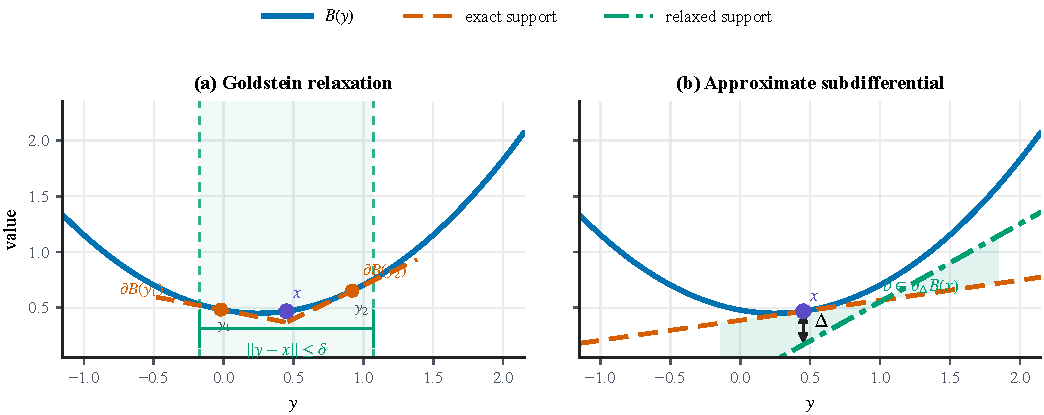
\includegraphics[width=\textwidth]{goldstein_vs_approximate_subdifferential.pdf}
   \caption{The Goldstein subdifferential $\partial^G_\delta$ and the
$\delta$-subdifferential $\partial_\delta$ relax exact stationarity along different axes. The former convexifies exact subgradients collected over the ball $\mathcal{B}_\delta(\bar{\bx})$ (a spatial enlargement), while the
latter fixes the base point and tolerates a Fenchel--Young gap of at most
$\delta$ in the supporting inequality (a value relaxation).}
    \label{fig:goldstein-vs-approximate-subdifferential}
\end{figure}


\section{Convergence Criteria for Nonsmooth DC Optimization}
\label{sec:dc-convergence-criteria}

\subsection{Criticality and $\varepsilon$-criticality}
\label{sec:finite-time-barrier}
A point $\bar\bx$ is called a \emph{critical point} of Problem~\eqref{prob:main} if
\begin{equation}
    \label{def:dc-critical}
    \zero\in \partial\phi(\bar\bx)-\partial g(\bar\bx).
\end{equation}
Equivalently, there exist $\bu\in\partial\phi(\bar\bx)$ and $\bv\in\partial g(\bar\bx)$ such that $\bu=\bv$. When both convex components are finite and locally Lipschitz around $\bar\bx$, the Clarke calculus gives $\partial_C F(\bar\bx) \subseteq \partial\phi(\bar\bx)-\partial g(\bar\bx)$. Hence, any local minimizer $\bar\bx$ of $F=\phi-g$ satisfies
\[
    \zero\in\partial_C F(\bar\bx) \subseteq \partial\phi(\bar\bx)-\partial g(\bar\bx).
\]

Exact same-point DC criticality is decomposition-dependent and may be
 weaker than Clarke stationarity of the difference function. For
example, let
\[
    \phi(x)=|x|,\qquad g(x)=|x|+x .
\]
Then \(\Psi=\phi-g=-x\), and hence
\[
    \partial_C\Psi(0)=\{-1\},
\]
so \(0\notin\partial_C\Psi(0)\). However,
\[
    \partial\phi(0)=[-1,1],\qquad \partial g(0)=[0,2],
\]
and therefore
\[
    0\in \partial\phi(0)-\partial g(0).
\]
Thus \(x=0\) is DC-critical for this particular decomposition even though
it is not Clarke-stationary for \(\Psi\). This example shows that a
finite-time lower bound for exact DC criticality cannot be obtained by
directly invoking lower bounds for pointwise Clarke stationarity of
\(\Psi\). The lower-bound construction must instead be carried out at the
level of the DC pair \((\phi,g)\) and the residual
\[
    \operatorname{dist}\bigl(0,\partial\phi(x)-\partial g(x)\bigr).
\]
% For this reason, our hard instance is built in two layers. A disjoint-kink
% background pair keeps every queried point's DC residual bounded away from
% zero, by the same resisting-oracle mechanism used at the Clarke level. A
% second, common-kink layer is then grafted onto both convex components at a
% single hidden location: it leaves the objective $F=\phi-g$, its Lipschitz
% constant, and its optimality gap completely unchanged, yet it enlarges
% $\partial\phi(x)-\partial g(x)$ at that location into a set containing
% zero, producing a point that is DC-critical without being Clarke
% stationary for $F$. This second layer is what makes the lower bound
% genuinely exercise the fact that DC criticality is weaker than Clarke
% stationarity, rather than inheriting hardness only because the two notions
% happen to coincide on the instance.

Given $\varepsilon>0$, a natural finite-time goal is the $\varepsilon$-criticality condition:
\begin{equation}
    \label{eq:exact-dc-eps-criticality}
    \operatorname{dist}\!\left( \zero, \partial\phi(\bar\bx)-\partial g(\bar\bx) \right) \le \varepsilon.
\end{equation}
This equivalently requires the existence of $\bu\in\partial\phi(\bar\bx)$ and $\bv\in\partial g(\bar\bx)$ such that $\|\bu-\bv\|\le \varepsilon$.

For comparison, the $\varepsilon$-stationarity condition for a locally Lipschitz nonsmooth nonconvex objective $F$ is $\operatorname{dist}\bigl(\zero,\partial_C F(\bar\bx)\bigr) \le \varepsilon$. Since $\partial_C F(\bar\bx) \subseteq \partial\phi(\bar\bx)-\partial g(\bar\bx)$, we have
\[
    \operatorname{dist}\!\left( \zero, \partial\phi(\bar\bx)-\partial g(\bar\bx) \right) \le \operatorname{dist}\bigl(\zero,\partial_C F(\bar\bx)\bigr).
\]
Thus, \eqref{eq:exact-dc-eps-criticality} serves as a decomposition-dependent DC analogue of Clarke $\varepsilon$-stationarity, and it ism weaker.

Zhang et al.~\citep{Zhang-2020-Complexity} established that for a broad class of Lipschitz nonsmooth nonconvex functions, no finite-time first-order algorithm can guarantee finding a point satisfying $\operatorname{dist}\bigl(\zero,\partial_C F(\bx)\bigr) \le \varepsilon$. For DC optimization, this limitation need to be re-evaluated for two reasons:
\begin{itemize}
\item[(Q1)] \emph{The DC oracle is stronger.} A DCA-type method may
query $\partial\phi$ and $\partial g$ \emph{separately}, and may even
observe $\phi(x)$ and $g(x)$ individually, whereas the obstruction of
\citet[Theorem~5]{Zhang-2020-Complexity} grants only one generalized
gradient of the whole objective. Since more information can only make
the problem easier, the lower bound is not inherited automatically.
\item[(Q2)] \emph{The DC measure is weaker.} The DC calculus gives
$\partial_C(\phi-g)(x)\subseteq\partial\phi(x)-\partial g(x)$, hence
\[
 \operatorname{dist}\bigl(0,\partial\phi(x)-\partial g(x)\bigr)
 \le
 \operatorname{dist}\bigl(0,\partial_C(\phi-g)(x)\bigr).
\]
Thus DC criticality is \emph{easier} to satisfy than Clarke
stationarity, so proving that even this weaker target is unattainable is
a strictly stronger statement than
\citet[Theorem~5]{Zhang-2020-Complexity}, not a corollary of it. A
construction whose DC residual and Clarke residual coincide everywhere
-- such as one built purely from disjoint component kinks -- proves the
Clarke-level statement but never actually tests (Q2), since the DC
target set is never larger than the Clarke target set on such an
instance. The construction below is designed so that (Q2) is tested
directly, at an explicit point where the two residuals differ.
\end{itemize}

The relevant question is whether finite-time $\varepsilon$-criticality can be achieved under this stronger DC oracle. Unfornunately, the answer is negative, as we show next. 
We settle both on a single explicit instance which is different from the hard instance constructed in \cite{Zhang-2020-Complexity}.

We formulate the lower bound under the setting where the pair $(\phi,g)$ is explicitly provided as problem data, granting the algorithm separate access to both convex components. \blue{Throughout this paper, we focus on the following subset of Lipschitz functions. For $\Delta,L,G>0$ and a fixed initial point $\bx^0$, we define:}
\[
\begin{aligned}
\mathcal D(\Delta,L,G) := \Bigl\{ (\phi,g):\;& \phi,g \text{ are proper, closed, convex, and finite-valued},\\
& F:=\phi-g \text{ is } L\text{-Lipschitz and Hadamard directionally differentiable},\\
& F(\bx^0)-\inf\limits_{\bx}F(\bx)\le \Delta,\\
& \sup\limits_{\bx} \sup\limits_{\bu\in\partial\phi(\bx),\,\bv\in\partial g(\bx)} \max\limits\{\|\bu\|,\|\bv\|\} \le G \Bigr\}.
\end{aligned}
\]
We then consider the \emph{strong} DC first-order oracle, which returns
both component values in addition to both component subgradients:
\[
    \mathcal O_{\rm DC}(\bx) = \bigl( \phi(\bx),\,g(\bx),\,\bu,\,\bv \bigr), \qquad \bu\in\partial\phi(\bx),\quad \bv\in\partial g(\bx).
\]
This dominates the weaker oracle $\bigl(F(\bx),\bu,\bv\bigr)$ used above, since $F(\bx)=\phi(\bx)-g(\bx)$ is recoverable from it; a lower bound against $\mathcal O_{\rm DC}$ is therefore the stronger statement required by (Q1). We make this claim precise as follows.
\begin{theorem}
\label{thm:dc-oracle-limitation-sketch}
Fix $\Delta,L,G>0$. There exists an absolute constant $c>0$ such that for every query budget $K\le cG/L$, every $\varepsilon\in(0,L)$, and every algorithm $\mathcal{A}$ interacting with the oracle $\mathcal O_{\rm DC}$, there exists a pair $(\phi,g)\in\mathcal D(\Delta,L,G)$ such that, with probability at least $1/2$, none of the first $K$ points $\{\bx^k\}_{k=1}^K$ queried by $\mathcal{A}$ is $\varepsilon$-critical:
\[
    \operatorname{dist}\!\left(
        \zero,\,
        \partial\phi(\bx^k)-\partial g(\bx^k)
    \right)
    >
    \varepsilon,
    \qquad k=1,\ldots,K.
\]
Moreover, the constructed pair contains a point $s$ with
\[
    \zero\in\partial\phi(s)-\partial g(s),
    \qquad
    \zero\notin\partial_C(\phi-g)(s).
\]
\end{theorem}

\begin{remark}
\label{rmk:GK-tradeoff}
Equivalently, for every $K$ the same construction gives a hard pair in $\mathcal D(\Delta,L,G_K)$ with $G_K=O(KL)$: each hidden background kink forces a slope jump in whichever convex component carries it, and monotonicity of a one-dimensional convex subgradient means these jumps accumulate rather than cancel. This $K$-dependence is specific to the one-dimensional construction; it is not present in the underlying Clarke-level obstruction of \citet{Zhang-2020-Complexity}, which does not need to keep two components separately bounded. 
% Removing the horizon restriction while keeping $G$ fixed for arbitrary $K$ would require a higher-dimensional zero-chain construction, which we leave for future work since the present statement already suffices to motivate the relaxed criticality measure introduced next.
\end{remark}
The hard instance has two layers, detailed in
\Cref{Appendix: Finite-Time Barriers of DC}.
\begin{proof}[Proof sketch]
We first construct a DC pair $(\phi_0,g_0)$ by decompositing the 
resisting-oracle construction in \citet{Zhang-2020-Complexity}.
% : given the
% $K$ queried points, it places hidden kinks between them so that every
% queried point has DC residual equal to a fixed gap $L>\varepsilon$. This
% layer is fixed once its geometric parameter is chosen; no part of it is
% hidden from the algorithm.

A common-kink layer $c_s(x)=M|x-s|+\beta-Ms$ is then added identically to
both components, $\phi_s=\phi_0+c_s$ and $g_s=g_0+c_s$. Because the same
term is added to both sides, $F=\phi_s-g_s=\phi_0-g_0$ is completely
unaffected by $s$: its Lipschitz constant, its optimality gap, and its
Clarke subdifferential everywhere are independent of $s$. Choosing the
intercept $\beta-Ms$ so that $c_s$ agrees with a fixed, $s$-independent
affine function at every point to the left of $s$ makes the entire
strong-oracle transcript -- both component values and both component
subgradients -- identical at every queried point, for every admissible
hidden location $s$ beyond the largest queried point. At $x=s$ itself,
the common kink enlarges $\partial\phi_s(s)-\partial g_s(s)$ into an
interval containing zero while leaving $\partial_C(\phi_s-g_s)(s)$
unchanged, producing the point promised in the theorem.

A two-instance argument over locations $s\neq s'$, both consistent with
the same $K$-query transcript, then shows that no algorithm can
guarantee success against both simultaneously, giving the stated
probability bound.
\end{proof}

\subsection{A Unified Notion of Approximate Criticality}
\label{sec:criticality}
In this section, we propose a unified notion to measure approximate criticality. We first recall the standard \(\delta\)-subdifferential of a proper closed convex function.

If $h:\RR^n\to\RR\cup\{+\infty\}$ is a convex function and $\delta > 0$, then for $\bar{\bx}\in\operatorname{dom} h$, the $\delta$-subdifferential of $h$ at $\bar{\bx}$ is defined by
\[
    \partial_\delta h(\bar{\bx})
    :=
    \left\{
    \bv\in\RR^n:
    h(\bz)\ge h(\bar{\bx})
    +\langle \bv,\bz-\bar{\bx}\rangle-\delta,
    \quad \forall \bz\in\RR^n
    \right\}.
\] 
When $\delta=0$, it reduces to the standard convex subdifferential. 
Figure~\ref{fig:epsilon_subgradient} illustrates that $\delta$ acts as a vertical relaxation of the supporting affine function in the geometric interpretation of the $\delta$-subgradient.

We first record the Fenchel-gap characterization of the
$\delta$-subdifferential below.
\begin{lemma}
\label{lem:fenchel-gap-toolkit}
Let $h:\RR^n\to\RR\cup\{+\infty\}$ be proper, closed, and convex, let
$\bar\bx\in\dom h$, and let $\bv\in\RR^n$, $\delta\ge0$. Then
\[
    \bv\in\partial_\delta h(\bar\bx)
    \quad\Longleftrightarrow\quad
    \Phi_h(\bar\bx,\bv)\le\delta .
\]
Moreover, $\Phi_h(\bar\bx,\bv)\ge0$ for every $\bv\in\RR^n$, and
$\bv\in\partial h(\bar\bx)$ if and only if $\Phi_h(\bar\bx,\bv)=0$.
\end{lemma}

\begin{proof}
By definition, $\bv\in\partial_\delta h(\bar\bx)$ if and only if
\begin{equation}
    h(\bz)\;\ge\;h(\bar\bx)+\langle\bv,\bz-\bar\bx\rangle-\delta
    \qquad\text{for all }\bz\in\RR^n,
    \label{eq:delta-subgrad-ineq}
\end{equation}
which, upon rearrangement, is equivalent to
\[
    \langle\bv,\bz\rangle-h(\bz)
    \;\le\;
    \langle\bv,\bar\bx\rangle-h(\bar\bx)+\delta
    \qquad\text{for all }\bz\in\RR^n.
\]
Taking the supremum over $\bz\in\RR^n$ on the left-hand side yields
$h^*(\bv)\le\langle\bv,\bar\bx\rangle-h(\bar\bx)+\delta$, that is,
$\Phi_h(\bar\bx,\bv)=h(\bar\bx)+h^*(\bv)-\langle\bv,\bar\bx\rangle
\le\delta$. Conversely, if $\Phi_h(\bar\bx,\bv)\le\delta$, then for every
$\bz\in\RR^n$,
\[
    \langle\bv,\bz\rangle-h(\bz)
    \;\le\;
    h^*(\bv)
    \;\le\;
    \langle\bv,\bar\bx\rangle-h(\bar\bx)+\delta,
\]
and rearranging recovers \eqref{eq:delta-subgrad-ineq}. The inequality
$\Phi_h(\bar\bx,\bv)\ge0$ is the Fenchel--Young inequality, and the case
$\delta=0$ gives the equality characterization of $\partial h(\bar\bx)$.
\end{proof}


\begin{figure}[t]
    \centering
    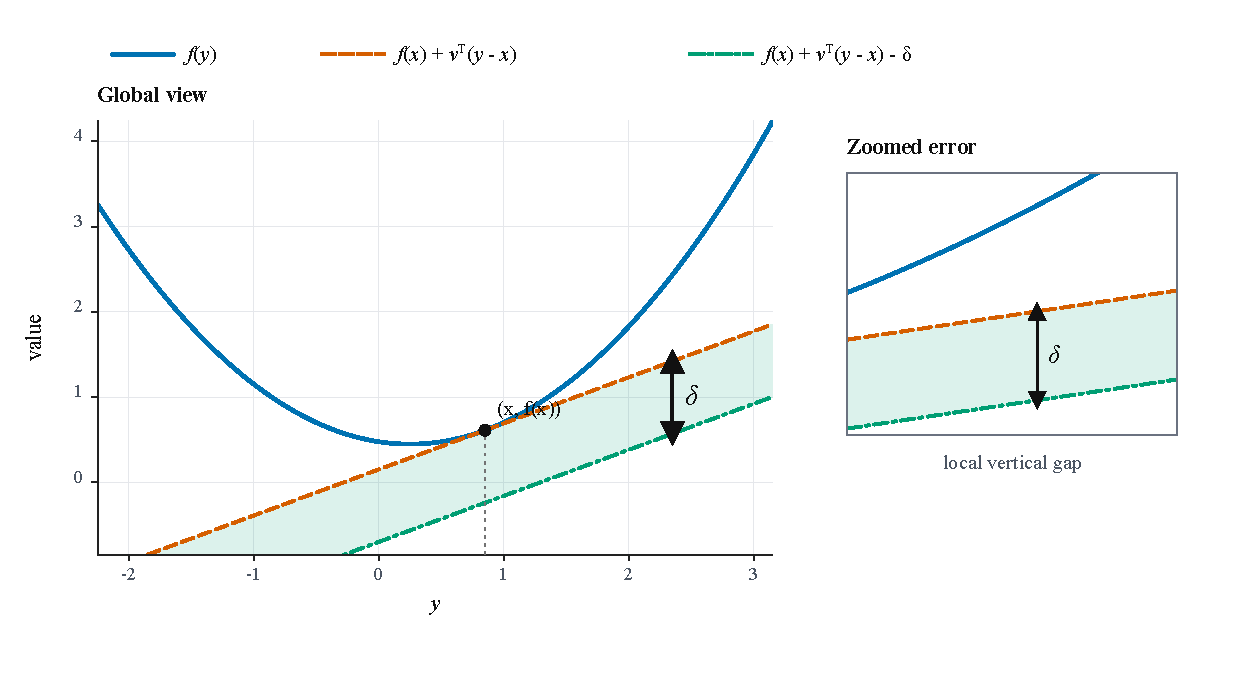
\includegraphics[width=0.7\textwidth]{epsilon_subgradient.pdf}
    \caption{Geometric interpretation of the $\delta$-subgradient. The green affine function is the ordinary supporting affine function shifted downward by $\delta$.}
    \label{fig:epsilon_subgradient}
\end{figure}

Given the limitations established in \Cref{thm:dc-oracle-limitation-sketch}, we relax the standard notion of criticality. By seeking a point in the proximity of an $\varepsilon$-critical point rather than an exact one, we are motivated to adopt the following unified definition of a $(\delta_{\phi},\delta_g,\varepsilon)$-critical point.

\begin{definition}[$(\delta_{\phi},\delta_g,\eps)$-critical point]
\label{def:delta-eps-critical}
Given \(\delta_{\phi},\delta_g\ge 0\) and \(\eps > 0\),
a point \(\bar{\bx}\in\operatorname{dom}\phi\cap\operatorname{dom}g\) is called a \((\delta_{\phi},\delta_g,\eps)\)-critical point of Problem \eqref{prob:main} if
\[
    \operatorname{dist}
    \left(
        \partial_{\delta_{\phi}}\phi(\bar{\bx}),
        \partial_{\delta_g}g(\bar{\bx})
    \right)
    \le \eps .
\]
\end{definition}


Based on this definition, we introduce the following gap functions to quantify the deviation from exact DC criticality:
\[
\begin{aligned}
    \Phi_{\phi}(\bx,\bu)
    &:=
    \phi(\bx)+\phi^*(\bu)-\langle \bu,\bx\rangle,
    \\
    \Phi_g(\bx,\bv)
    &:=
    g(\bx)+g^*(\bv)-\langle \bv,\bx\rangle.
\end{aligned}
\]

Observe that exact criticality is equivalent to the existence of a single dual vector $\bv$ such that both gap functions vanish, i.e., \(\exists \bv\) such that \(\Phi_{\phi}(\bx,\bv)=0\) and \(\Phi_g(\bx,\bv)=0\). In contrast, the $(\delta_{\phi},\delta_g,\eps)$-critical point in \Cref{def:delta-eps-critical} allows for different approximate subgradients on the two convex components, alongside a bounded mismatch between these dual vectors:
\[
\begin{aligned}
    \exists \bu,\bv,\qquad
    \Phi_{\phi}(\bx,\bu)\le \delta_{\phi},\quad
    \Phi_g(\bx,\bv)\le \delta_g, \quad 
    \|\bu-\bv\|\le \eps .
\end{aligned}
\]

When $\delta_{\phi}=\delta_g=0$, the $(0,0,\eps)$-critical point reduces to the classical $\varepsilon$-critical point. In fact, the $(\delta_{\phi},\delta_g,\eps)$-criticality serves as a more reliable diagnostic metric for approximate criticality. For nonsmooth DC functions, classical point-based stationarity residuals can remain stubbornly large ($\mathcal{O}(1)$) near a nonsmooth minimizer, whereas our proposed Fenchel-gap metric smoothly converges to zero. The following one-dimensional, closed-form example makes this diagnostic obstruction explicit.

\begin{figure}[t]
\centering
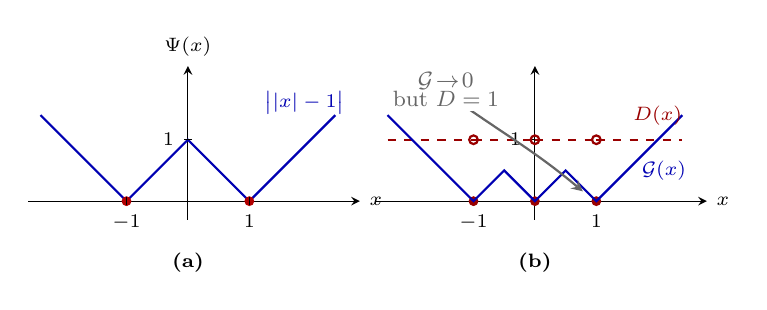
\begin{tikzpicture}[>=stealth, font=\scriptsize, scale=0.78]
 
% ================================================================
% Panel (a):  Psi(x) = ||x|-1|
% ================================================================
\begin{scope}[xshift=0cm]
 
  % axes
  \draw[->] (-2.6,0) -- (2.8,0) node[right] {$x$};
  \draw[->] (0,-0.3) -- (0,2.2) node[above] {$\Psi(x)$};
 
  % Psi(x) = ||x|-1|
  % key points: (-2,1) (-1,0) (0,1) (1,0) (2,1)
  \draw[thick, blue!70!black]
    (-2.4,1.4) -- (-1,0) -- (0,1) -- (1,0) -- (2.4,1.4);
 
  % mark minimizers
  \filldraw[red!70!black] (-1,0) circle (2pt);
  \filldraw[red!70!black] ( 1,0) circle (2pt);
 
  % tick marks
  \draw (-1,0.07) -- (-1,-0.07) node[below] {$-1$};
  \draw ( 1,0.07) -- ( 1,-0.07) node[below] {$1$};
  \draw (0.07,1) -- (-0.07,1) node[left] {$1$};
 
  % label
  \node[blue!70!black] at (1.9,1.6) {$\bigl||x|-1\bigr|$};
 
  % panel label
  \node at (0,-1.0) {\textbf{(a)}};
 
\end{scope}
 
% ================================================================
% Panel (b):  D(x) vs G(x)
% ================================================================
\begin{scope}[xshift=5.65cm]
 
  % axes
  \draw[->] (-2.6,0) -- (2.8,0) node[right] {$x$};
  \draw[->] (0,-0.3) -- (0,2.2);
 
  % tick marks
  \draw (-1,0.07) -- (-1,-0.07) node[below] {$-1$};
  \draw ( 1,0.07) -- ( 1,-0.07) node[below] {$1$};
  \draw (0.07,1) -- (-0.07,1) node[left] {$1$};
 
  % --- D(x): dashed, step function at 1, with jumps at {-1,0,1} ---
  \draw[thick, dashed, red!60!black]
    (-2.4,1) -- (-1,1);
  \draw[thick, dashed, red!60!black]
    (-1,1) -- (0,1);
  \draw[thick, dashed, red!60!black]
    (0,1) -- (1,1);
  \draw[thick, dashed, red!60!black]
    (1,1) -- (2.4,1);
 
  % open circles at D=1 for x in {-1,0,1}
  \draw[red!60!black, thick] (-1,1) circle (2pt);
  \draw[red!60!black, thick] ( 0,1) circle (2pt);
  \draw[red!60!black, thick] ( 1,1) circle (2pt);
 
  % closed circles at D=0 for x in {-1,0,1}
  \filldraw[red!60!black] (-1,0) circle (2pt);
  \filldraw[red!60!black] ( 0,0) circle (2pt);
  \filldraw[red!60!black] ( 1,0) circle (2pt);
 
  % --- G(x): solid, piecewise linear ---
  % G(x) = |x|              for 0<=|x|<=1/2
  %       = 1-|x|           for 1/2<=|x|<=1
  %       = |x|-1           for |x|>=1
  % key points: (-2,1) (-1,0) (-0.5,0.5) (0,0) (0.5,0.5) (1,0) (2,1)
  \draw[thick, blue!70!black]
    (-2.4,1.4) -- (-1,0) -- (-0.5,0.5) -- (0,0)
    -- (0.5,0.5) -- (1,0) -- (2.4,1.4);
 
  % labels
  \node[red!60!black]  at (2.0, 1.4) {$D(x)$};
  \node[blue!70!black] at (2.1, 0.5) {$\mathcal{G}(x)$};
 
  % annotation arrow: highlight the gap near x=1
  \draw[->, thick, black!60] (-1.25,1.62) to[out=-35,in=140] (0.78,0.16);
  \node[black!60, align=center, fill=white, inner sep=1.5pt]
    at (-1.45,1.82)
    {\footnotesize $\mathcal{G}\!\to\!0$\\[-1pt]\footnotesize but $D=1$};
 
  % panel label
  \node at (0,-1.0) {\textbf{(b)}};
 
\end{scope}
\end{tikzpicture}
\caption{Exact critical-distance residual versus Fenchel-gap behavior in the one-dimensional example.}
\label{fig:exact-vs-fenchel-gap}
\end{figure}

\begin{example}[Exact vs.\ Fenchel-gap certificate]
\label{ex:motivating-dc-gap}
Consider
\[
    \Psi(x)=\bigl||x|-1\bigr|
    =
    \phi(x)-g(x),
\]
where \( \phi(x)=3+4(|x|-1)_+ \) and \( g(x)=|x+1|+|x|+|x-1| \). Both \(\phi\) and \(g\) are convex, and \(g\) is nonsmooth at the global minimizers \(x=\pm1\). The exact same-point critical-distance residual is
\[
    D(x)
    :=
    \operatorname{dist}\bigl(0,\partial\phi(x)-\partial g(x)\bigr)
    =
    \begin{cases}
    0, & x\in\{-1,0,1\},\\
    1, & \text{otherwise}.
    \end{cases}
\]
Hence, even when \(x\) is arbitrarily close to the nonsmooth minimizer \(x=1\), the exact critical distance remains \(D(x)=1\).

For comparison, specialize the two-sided Fenchel certificate to the common-certificate scalar gap
\[
    \calG(x)
    :=
    \inf\limits_{b\in\RR}
    \left\{
        \Phi_\phi(x,b)+\Phi_g(x,b)
    \right\}.
\]
This corresponds to the case \(\bu=\bv=b\): the same scalar \(b\) must act as an approximate subgradient certificate for both convex components at the same point. A direct conjugate calculation gives
\[
\begin{aligned}
    \phi^*(b)
    &=
    \begin{cases}
        |b|-3, & |b|\le 4,\\
        +\infty, & |b|>4,
    \end{cases}
    \\
    g^*(b)
    &=
    \begin{cases}
        -2, & |b|\le 1,\\
        |b|-3, & 1\le |b|\le 3,\\
        +\infty, & |b|>3.
    \end{cases}
\end{aligned}
\]
Consequently,
\[
    \calG(x)
    =
    \begin{cases}
        |x|, & 0\le |x|\le \frac12,\\
        1-|x|, & \frac12\le |x|\le 1,\\
        |x|-1, & |x|\ge 1.
    \end{cases}
\]
In particular, \(\calG(x)\to0\) as \(x\to\pm1\), while \(D(x)=1\) for every \(x\notin\{-1,0,1\}\). Equivalently, near \(x=1\), choosing \(b=1\in\partial g(x)\) for \(0<x<1\) gives
\[
    \Phi_g(x,1)=0,
    \qquad
    \Phi_\phi(x,1)=1-x\to0
    \;\;\text{as }x\uparrow1,
\]
and choosing \(b=3\in\partial g(x)\) for \(x>1\) gives
\[
    \Phi_g(x,3)=0,
    \qquad
    \Phi_\phi(x,3)=x-1\to0
    \;\;\text{as }x\downarrow1.
\]
This is the behavior shown in \Cref{fig:exact-vs-fenchel-gap}: the Fenchel gap accurately detects convergence toward a nonsmooth minimizer, whereas the exact critical distance remains an \(O(1)\) step function around it.
\end{example}

\Cref{ex:motivating-dc-gap} shows that the $(\delta_\phi,\delta_g,\varepsilon)$-critical point repairs the diagnostic failure of the exact residual, but a diagnostic that is easy to satisfy is only useful if it is also sound: an overly permissive relaxation could remain satisfiable at points bearing no relation to criticality at all. We close this section by ruling out this concern as follows.
 The next proposition shows that \Cref{def:delta-eps-critical} degenerates correctly, in the sense that driving all three tolerances to zero forces exact DC criticality at the same point.
This properpsition depends on the monotonicity of the $\delta$-subdifferential in $\delta$ together with lower semicontinuity of $\phi,\phi^*,g,g^*$; 

\begin{proposition}
\label{prop:exact-consistency}
Suppose $\phi$ and $g$ are $G$-Lipschitz on $\RR^n$. If $\bar\bx$ is a $(\delta_\phi^{(k)},\delta_g^{(k)},\varepsilon^{(k)})$-critical point of Problem~\eqref{prob:main} for every $k\in\NN$, with $\delta_\phi^{(k)},\delta_g^{(k)},\varepsilon^{(k)}\to0$ as $k\to\infty$, then $\bar\bx$ is a critical point of Problem~\eqref{prob:main}, i.e., $\zero\in\partial\phi(\bar\bx)-\partial g(\bar\bx)$.
\end{proposition}

\begin{proof}
For each $k$, choose $\bu_k\in\partial_{\delta_\phi^{(k)}}\phi(\bar\bx)$ and $\bv_k\in\partial_{\delta_g^{(k)}}g(\bar\bx)$ with $\|\bu_k-\bv_k\|\le\varepsilon^{(k)}$. Since $\phi$ is $G$-Lipschitz on all of $\RR^n$, every element of $\partial_\delta\phi(\bar\bx)$ has norm at most $G$, regardless of $\delta$: for $\bv\in\partial_\delta\phi(\bar\bx)$, the defining inequality $\phi(\bar\bx)+G\|\bz-\bar\bx\|\ge\phi(\bz)\ge\phi(\bar\bx)+\langle\bv,\bz-\bar\bx\rangle-\delta$ along $\bz-\bar\bx=t\bv/\|\bv\|$ forces $\|\bv\|\le G+\delta/t$ for every $t>0$, hence $\|\bv\|\le G$ as $t\to\infty$. The same bound holds for $\partial_\delta g(\bar\bx)$. Thus $\{\bu_k\}$ and $\{\bv_k\}$ are bounded, and we may pass to a subsequence along which $\bu_k\to\bu^\star$ and $\bv_k\to\bv^\star$; since $\|\bu_k-\bv_k\|\to0$, we get $\bu^\star=\bv^\star=:\bw$.

It remains to show $\bw\in\partial\phi(\bar\bx)$; the argument for $\bw\in\partial g(\bar\bx)$ is identical. Since $\phi$ and $\phi^*$ are proper, closed, and convex, both are lower semicontinuous, so
\[
    \Phi_\phi(\bar\bx,\bw)
    =\phi(\bar\bx)+\phi^*(\bw)-\langle\bw,\bar\bx\rangle
    \le\liminf_{k\to\infty}\Bigl[\phi(\bar\bx)+\phi^*(\bu_k)-\langle\bu_k,\bar\bx\rangle\Bigr]
    =\liminf_{k\to\infty}\Phi_\phi(\bar\bx,\bu_k)
    \le\liminf_{k\to\infty}\delta_\phi^{(k)}=0.
\]
The Fenchel--Young inequality gives $\Phi_\phi(\bar\bx,\bw)\ge0$ unconditionally, so $\Phi_\phi(\bar\bx,\bw)=0$, i.e., $\bw\in\partial\phi(\bar\bx)$. Hence $\bw\in\partial\phi(\bar\bx)\cap\partial g(\bar\bx)$, and $\zero=\bw-\bw\in\partial\phi(\bar\bx)-\partial g(\bar\bx)$.
\end{proof}


% no spatial displacement argument is needed, since the collapse takes place at the fixed point $\bar\bx$. This is a first indication of a recurring theme in \Cref{sec:relationship-relaxed-dc-criticality} below: relaxing criticality along the value axis, rather than the spatial axis, tends to keep the base point fixed throughout.

\subsection{Relationship between Relaxed DC Criticality Notions}
\label{sec:relationship-relaxed-dc-criticality}

We show that the $(\delta_\phi,\delta_g,\varepsilon)$-critical point in
\Cref{def:delta-eps-critical} is a unifying value-relaxed formulation:
every previously proposed relaxed DC criticality notion for
Problem~\eqref{prob:main} embeds into
\Cref{def:delta-eps-critical} for a suitable choice of
$(\delta_\phi,\delta_g,\varepsilon)$, and this embedding admits a sharper,
second-order accurate rate whenever the underlying component is smooth.

We recall three such notions, in increasing order of the spatial freedom
they allow.

\begin{definition}[$\varepsilon$-critical point~\citep{moudafi2021complete,sun2023algorithms}]
\label{Def: epsilon-critical point in DC}
Given $\varepsilon>0$, a point $\bar\bx\in\RR^n$ is an $\varepsilon$-critical
point of Problem~\eqref{prob:main} if there exist
$\bar\by\in\RR^n$ and $\bar\bu\in\partial\phi(\bar\bx)-\partial g(\bar\by)$
such that
\[
    \max\limits\{\|\bar\bu\|,\|\bar\bx-\bar\by\|\}\le\varepsilon .
\]
\end{definition}

\begin{definition}[Nearly $\varepsilon$-critical point~\citep{yao2022large}]
\label{Def: epsilon-critical point 3}
Given $\varepsilon>0$, a point $\bar\bx\in\RR^n$ is a nearly
$\varepsilon$-critical point of Problem~\eqref{prob:main}
if there exist $\bar\by_1,\bar\by_2\in\RR^n$ and
$\bar\bu\in\partial\phi(\bar\by_1)-\partial g(\bar\by_2)$ such that
\[
    \max\limits\{\|\bar\bu\|,\|\bar\bx-\bar\by_1\|,\|\bar\bx-\bar\by_2\|\}
    \le\varepsilon .
\]
\end{definition}

\begin{definition}[Nearly $\varepsilon$-stationary point~\citep{xu2019stochastic}]
\label{def:xu-near-stationary}
Given $\varepsilon>0$, a point $\bar\bx\in\RR^n$ is a nearly
$\varepsilon$-stationary point of Problem~\eqref{prob:main} if there exist
$c>0$ and $\bx^*\in\RR^n$ with
$\|\bar\bx-\bx^*\|\le c\varepsilon$ such that
\[
    \operatorname{dist}\bigl(\partial\phi(\bx^*),\partial g(\bx^*)\bigr)
    \le\varepsilon .
\]
\end{definition}

Definitions~\ref{Def: epsilon-critical point in DC} and
\ref{Def: epsilon-critical point 3} relax criticality by letting $\phi$
and $g$ be evaluated at points that may drift apart from each other and
from $\bar\bx$; \Cref{def:xu-near-stationary} instead forces $\phi$ and
$g$ to share a common witness point $\bx^*$, which itself may drift from
$\bar\bx$. All three reduce to a single mechanism: converting a spatial
offset into a Fenchel-gap slack.

\begin{lemma}
\label{lem:spatial-to-value}
Let $q:\RR^n\to\RR\cup\{+\infty\}$ be proper, closed, convex, and
$G$-Lipschitz on a convex set containing $\bx,\by\in\operatorname{dom}q$.
\begin{enumerate}
    \item[(a)] If $\bv\in\partial q(\by)$, then
    $\bv\in\partial_{2G\|\bx-\by\|}q(\bx)$.
    \item[(b)] If, in addition, $q$ is $L$-smooth on this set and
    $\bv=\nabla q(\by)$, then
    $\bv\in\partial_{\frac{L}{2}\|\bx-\by\|^2}q(\bx)$.
\end{enumerate}
\end{lemma}

\begin{proof}
By the Fenchel--Young equality at a subgradient,
$q^*(\bv)=\langle\bv,\by\rangle-q(\by)$, so
\[
    \Phi_q(\bx,\bv)
    = q(\bx)-q(\by)-\langle\bv,\bx-\by\rangle
    =: D_q(\bx,\by).
\]
(a) Convexity gives $D_q(\bx,\by)\ge0$; $G$-Lipschitzness gives
$q(\bx)-q(\by)\le G\|\bx-\by\|$ and $\|\bv\|\le G$, so
$D_q(\bx,\by)\le 2G\|\bx-\by\|$.
(b) $D_q(\bx,\by)$ is the Bregman divergence of $q$ at $(\bx,\by)$; for
convex $L$-smooth $q$ it satisfies $0\le D_q(\bx,\by)\le\tfrac
L2\|\bx-\by\|^2$ by the descent lemma.
\end{proof}
We then establish that the $(\delta_\phi,\delta_g,\varepsilon)$-critical point in \Cref{def:delta-eps-critical} recovers all three existing relaxed DC criticality notions
\begin{proposition}
\label{prop:recovery-existing-dc-criticality}
Suppose $\phi$ and $g$ are, respectively, $G_\phi$- and $G_g$-Lipschitz on
the relevant neighborhoods below. Then:
\begin{enumerate}
    \item[(i)] If $\bar\bx$ is an $\varepsilon$-critical point in the
    sense of \Cref{Def: epsilon-critical point in DC}, then $\bar\bx$ is a
    $(0,\,2G_g\varepsilon,\,\varepsilon)$-critical point.
    \item[(ii)] If $\bar\bx$ is a nearly $\varepsilon$-critical point in
    the sense of \Cref{Def: epsilon-critical point 3}, then $\bar\bx$ is a
    $(2G_\phi\varepsilon,\,2G_g\varepsilon,\,\varepsilon)$-critical point.
    \item[(iii)] If $\bar\bx$ is a nearly $\varepsilon$-stationary point in
    the sense of \Cref{def:xu-near-stationary}, then $\bar\bx$ is a
    $(2G_\phi c\varepsilon,\,2G_g c\varepsilon,\,\varepsilon)$-critical
    point.
\end{enumerate}
\end{proposition}

\begin{proof}
(i) Write $\bar\bu=\bp-\bq$ with $\bp\in\partial\phi(\bar\bx)
=\partial_0\phi(\bar\bx)$ and $\bq\in\partial g(\bar\by)$.
\Cref{lem:spatial-to-value}(a) with $q=g$, $\bx=\bar\bx$, $\by=\bar\by$
gives $\bq\in\partial_{2G_g\|\bar\bx-\bar\by\|}g(\bar\bx)\subseteq
\partial_{2G_g\varepsilon}g(\bar\bx)$, so
$\operatorname{dist}(\partial_0\phi(\bar\bx),\partial_{2G_g\varepsilon}g(\bar\bx))
\le\|\bp-\bq\|=\|\bar\bu\|\le\varepsilon$.

(ii) Identical, applying \Cref{lem:spatial-to-value}(a) to both
$\bp\in\partial\phi(\bar\by_1)$ and $\bq\in\partial g(\bar\by_2)$.

(iii) Take $\bp\in\partial\phi(\bx^*)$, $\bq\in\partial g(\bx^*)$ with
$\|\bp-\bq\|\le\varepsilon$; this is exactly case (ii) with
$\bar\by_1=\bar\by_2=\bx^*$ and spatial offset $c\varepsilon$ in place of
$\varepsilon$.
\end{proof}

\begin{remark}
Case (iii) is not an independent construction: it is case (ii)
specialized to a common witness point. The distinction between
\Cref{Def: epsilon-critical point in DC}/\ref{Def: epsilon-critical point 3}
and \Cref{def:xu-near-stationary} is therefore not a difference in the
relaxation mechanism, but only in whether the two witness points are
allowed to coincide.
\end{remark}

The embedding above only uses Lipschitz continuity and is tight up to
constants. When a component happens to be smooth,
\Cref{lem:spatial-to-value}(b) applies in place of (a) and yields a
second-order accurate slack on that side.

\begin{proposition}
\label{prop:sharp-smooth}
In the setting of \Cref{def:xu-near-stationary}, suppose in addition that
$g$ is convex and $L_g$-smooth on a neighborhood of $\bx^*$. Then
$\bar\bx$ is a
\[
    \Bigl(2G_\phi c\varepsilon,\ \tfrac{L_g}{2}c^2\varepsilon^2,\
    \varepsilon\Bigr)\text{-critical point}.
\]
If $\phi$ is also convex and $L_\phi$-smooth on a neighborhood of
$\bx^*$, the first slack sharpens to $\tfrac{L_\phi}{2}c^2\varepsilon^2$,
so that $\bar\bx$ is an
$\bigl(\mathcal O(\varepsilon^2),\,\mathcal O(\varepsilon^2),\,
\varepsilon\bigr)$-critical point.
\end{proposition}

\begin{proof}
Take $\bv^*=\nabla g(\bx^*)$ in place of an arbitrary
$\bq\in\partial g(\bx^*)$ in the proof of
\Cref{prop:recovery-existing-dc-criticality}(iii), and apply
\Cref{lem:spatial-to-value}(b) instead of (a):
$\bv^*\in\partial_{\frac{L_g}{2}\|\bar\bx-\bx^*\|^2}g(\bar\bx)
\subseteq\partial_{\frac{L_g}{2}c^2\varepsilon^2}g(\bar\bx)$. The
$\phi$-side bound is unchanged from
\Cref{prop:recovery-existing-dc-criticality}(iii). The refinement when
$\phi$ is also smooth follows by the same substitution on the
$\phi$-side.
\end{proof}

\Cref{prop:recovery-existing-dc-criticality} and
\Cref{prop:sharp-smooth} together show that
\Cref{def:delta-eps-critical} strictly subsumes
Definitions~\ref{Def: epsilon-critical point in DC},
\ref{Def: epsilon-critical point 3}, and \ref{def:xu-near-stationary}: the
value slack incurred is $\mathcal O(\varepsilon)$ under Lipschitz
continuity alone, and tightens to $\mathcal O(\varepsilon^2)$ on any
component that is additionally smooth. This also isolates precisely what
smoothness of $g$ buys in \citet{xu2019stochastic}: it is not needed for
the embedding into \Cref{def:delta-eps-critical}, which only requires
Lipschitz continuity, but it tightens the resulting slack by one order in
$\varepsilon$.

\subsubsection{The Converse Embedding}

\Cref{prop:recovery-existing-dc-criticality} and \Cref{prop:sharp-smooth}
show that $(\delta_\phi,\delta_g,\varepsilon)$-criticality is no harder to
satisfy than any previously proposed relaxed DC criticality notion. We now
establish the converse direction: satisfying \Cref{def:delta-eps-critical}
is also no easier, in the sense that it forces the same qualitative
conclusion as \Cref{Def: epsilon-critical point 3}, up to an explicit loss
of one order in the tolerance. The mechanism is the classical reachback
theorem of Brøndsted and Rockafellar~\citep{brondsted1965subdifferentiability},
which converts an approximate subgradient at $\bar\bx$ into an exact
subgradient at a nearby point, and is the exact converse of
\Cref{lem:spatial-to-value}(a).

\begin{lemma}
\label{lem:value-to-spatial}
Let $q:\RR^n\to\RR\cup\{+\infty\}$ be proper, closed, and convex, and let
$\bv\in\partial_\delta q(\bar\bx)$ for some $\delta>0$. Then for every
$\lambda>0$ there exist $\hat\bx\in\RR^n$ and $\hat\bv\in\partial
q(\hat\bx)$ such that
\[
    \|\hat\bx-\bar\bx\|\le\lambda,
    \qquad
    \|\hat\bv-\bv\|\le\frac{\delta}{\lambda}.
\]
In particular, taking $\lambda=\sqrt\delta$ gives
$\|\hat\bx-\bar\bx\|\le\sqrt\delta$ and $\|\hat\bv-\bv\|\le\sqrt\delta$.
\end{lemma}

\begin{proposition}[Reverse embedding]
\label{prop:reverse-embedding}
If $\bar\bx$ is a $(\delta_\phi,\delta_g,\varepsilon)$-critical point of
Problem~\eqref{prob:main}, then $\bar\bx$ is a nearly
$\varepsilon'$-critical point in the sense of
\Cref{Def: epsilon-critical point 3}, with
\[
    \varepsilon'=\varepsilon+\sqrt{\delta_\phi}+\sqrt{\delta_g}.
\]
\end{proposition}

\begin{proof}
Let $\bu\in\partial_{\delta_\phi}\phi(\bar\bx)$ and
$\bv\in\partial_{\delta_g}g(\bar\bx)$ with $\|\bu-\bv\|\le\varepsilon$.
Apply \Cref{lem:value-to-spatial} to $\bu$ with $\lambda=\sqrt{\delta_\phi}$
and to $\bv$ with $\lambda=\sqrt{\delta_g}$, obtaining $\bar\by_1$,
$\hat\bu\in\partial\phi(\bar\by_1)$ and $\bar\by_2$,
$\hat\bv\in\partial g(\bar\by_2)$ with $\|\bar\by_1-\bar\bx\|\le\sqrt{\delta_\phi}$,
$\|\hat\bu-\bu\|\le\sqrt{\delta_\phi}$, and analogously for
$\bar\by_2,\hat\bv$. Set $\bar\bu:=\hat\bu-\hat\bv\in\partial\phi(\bar\by_1)-\partial g(\bar\by_2)$. The triangle inequality gives
\[
    \|\bar\bu\|
    \le\|\hat\bu-\bu\|+\|\bu-\bv\|+\|\bv-\hat\bv\|
    \le\sqrt{\delta_\phi}+\varepsilon+\sqrt{\delta_g}=\varepsilon',
\]
while $\|\bar\bx-\bar\by_1\|\le\sqrt{\delta_\phi}\le\varepsilon'$ and
$\|\bar\bx-\bar\by_2\|\le\sqrt{\delta_g}\le\varepsilon'$, which verifies the
defining condition of \Cref{Def: epsilon-critical point 3} with
$\varepsilon'$ in place of $\varepsilon$.
\end{proof}

\begin{proposition}[Same-point refinement under smoothness]
\label{prop:reverse-smooth}
In the setting of \Cref{prop:reverse-embedding}, suppose in addition that
$g$ is convex and $L_g$-smooth on a neighborhood of $\bar\bx$. Then
\[
    \operatorname{dist}\bigl(\nabla g(\bar\bx),\,\partial_{\delta_\phi}\phi(\bar\bx)\bigr)
    \le\varepsilon+\sqrt{2L_g\delta_g}.
\]
If $\phi$ is also convex and $L_\phi$-smooth on a neighborhood of
$\bar\bx$, then
\[
    \bigl\|\nabla\phi(\bar\bx)-\nabla g(\bar\bx)\bigr\|
    \le\varepsilon+\sqrt{2L_\phi\delta_\phi}+\sqrt{2L_g\delta_g},
\]
so that $\bar\bx$ is, up to this explicit slack, a same-point approximate
stationary point of the smooth DC problem.
\end{proposition}

\begin{proof}
For $L_g$-smooth convex $g$, the conjugate $g^*$ is
$\tfrac1{L_g}$-strongly convex, so $\Phi_g(\bar\bx,\bv)\ge
\tfrac1{2L_g}\|\bv-\nabla g(\bar\bx)\|^2$ for every $\bv$. Applied to
$\bv\in\partial_{\delta_g}g(\bar\bx)$, this gives
$\|\bv-\nabla g(\bar\bx)\|\le\sqrt{2L_g\delta_g}$; combined with
$\bu\in\partial_{\delta_\phi}\phi(\bar\bx)$ and $\|\bu-\bv\|\le\varepsilon$,
the triangle inequality gives the first bound. The second bound follows by
the same argument applied to $\bu$ once $\phi$ is also $L_\phi$-smooth and
convex.
\end{proof}

\begin{remark}[Asymmetry between the two directions]
The two directions are not symmetric. Embedding an existing notion into
\Cref{def:delta-eps-critical} costs a value slack linear in the spatial
tolerance under Lipschitz continuity alone (\Cref{lem:spatial-to-value}(a))
and quadratic under smoothness (\Cref{lem:spatial-to-value}(b)). Recovering
an existing notion from \Cref{def:delta-eps-critical} costs a spatial
displacement on the order of the square root of the value tolerance under
Lipschitz continuity alone (\Cref{lem:value-to-spatial}); this square-root
rate is the classical Brøndsted--Rockafellar rate and is not, in general,
improvable to a linear one. Smoothness removes the asymmetry in the
strongest sense: on a smooth component, the reverse direction also
collapses to a same-point bound (\Cref{prop:reverse-smooth}), matching the
same-point character of the forward direction under smoothness
(\Cref{prop:sharp-smooth}), at the cost of a square-root rather than a
quadratic rate.
\end{remark}

\subsubsection{Relation to Goldstein Stationarity}

We conclude by relating $(\delta_\phi,\delta_g,\varepsilon)$-criticality to
a relaxed stationarity notion outside the DC literature: the Goldstein
$\delta$-subdifferential relaxation of Clarke stationarity
\citep{goldstein1977optimization,Zhang-2020-Complexity}, introduced
schematically in \Cref{fig:goldstein-vs-approximate-subdifferential}. For a
locally Lipschitz function $F:\RR^n\to\RR$, the Goldstein
$\delta$-subdifferential at $\bar\bx$ is
\[
    \partial_\delta^G F(\bar\bx)
    :=
    \overline{\operatorname{conv}}
    \bigcup_{\by\in B_\delta(\bar\bx)}
    \partial_C F(\by),
\]
and $\bar\bx$ is a $(\delta,\varepsilon)$-Goldstein stationary point of $F$
if $\operatorname{dist}(\zero,\partial_\delta^G F(\bar\bx))\le\varepsilon$,
where $B_\delta(\bar\bx):=\{\by\in\RR^n:\|\by-\bar\bx\|\le\delta\}$.
Applied to $F=\Psi=\phi-g$, this relaxes Clarke stationarity along the
spatial axis: it collects exact generalized gradients over a
$\delta$-neighborhood of $\bar\bx$ and convexifies, rather than relaxing
the defining inequality at $\bar\bx$ itself. \Cref{def:delta-eps-critical}
relaxes along the orthogonal, value axis, and couples $\phi$ and $g$
independently rather than through a common witness point in
$B_\delta(\bar\bx)$. \Cref{tab:goldstein-vs-ours} summarizes the
distinction.

\begin{table}[t]
\centering
\caption{Two relaxation mechanisms for the same base criterion
$\zero\in\partial\phi(\bar\bx)-\partial g(\bar\bx)$.}
\label{tab:goldstein-vs-ours}
\small
\begin{tabular}{lll}
\hline
 & $(\delta,\varepsilon)$-Goldstein & $(\delta_\phi,\delta_g,\varepsilon)$-critical \\
\hline
Relaxation axis & spatial, $B_\delta(\bar\bx)$ & value, Fenchel--Young gap \\
Witness structure & common $\by\in B_\delta(\bar\bx)$ & independent $\bu,\bv$ at $\bar\bx$ \\
Evaluation point & nearby $\by$ & $\bar\bx$ itself \\
\hline
\end{tabular}
\end{table}

Despite this structural difference, the Goldstein relaxation embeds into
ours.

\begin{lemma}[Goldstein bridge]
\label{cor:goldstein-bridge}
Let $q:\RR^n\to\RR\cup\{+\infty\}$ be proper, closed, convex, and
$G$-Lipschitz on a convex set containing $B_\delta(\bar\bx)$. Then
\[
    \bigcup_{\by\in B_\delta(\bar\bx)}\partial q(\by)
    \subseteq
    \partial_{2G\delta}q(\bar\bx).
\]
\end{lemma}

\begin{proof}
Immediate from \Cref{lem:spatial-to-value}(a): for $\by\in B_\delta(\bar\bx)$
and $\bv\in\partial q(\by)$, $\|\bar\bx-\by\|\le\delta$ gives
$\bv\in\partial_{2G\delta}q(\bar\bx)$.
\end{proof}

\begin{proposition}[Goldstein implies ours]
\label{prop:goldstein-implies-ours}
Suppose $\phi,g$ are, respectively, $G_\phi$- and $G_g$-Lipschitz on a
convex set containing $B_\delta(\bar\bx)$. If $\bar\bx$ is a
$(\delta,\varepsilon)$-Goldstein stationary point of $\Psi=\phi-g$, then
$\bar\bx$ is a $(2G_\phi\delta,\,2G_g\delta,\,\varepsilon)$-critical point.
\end{proposition}

\begin{proof}
Let $\bw\in\partial_\delta^G\Psi(\bar\bx)$ with $\|\bw\|\le\varepsilon$. By
Carath\'eodory's theorem, $\bw=\sum_i\lambda_i\bw_i$ for finitely many
$\bw_i\in\partial_C\Psi(\by_i)$, $\by_i\in B_\delta(\bar\bx)$,
$\lambda_i\ge0$, $\sum_i\lambda_i=1$. By the Clarke sum rule for the
difference of two convex functions, $\bw_i=\bu_i-\bv_i$ with
$\bu_i\in\partial\phi(\by_i)$, $\bv_i\in\partial g(\by_i)$. Set
$\bar\bu:=\sum_i\lambda_i\bu_i$ and $\bar\bv:=\sum_i\lambda_i\bv_i$. By
\Cref{cor:goldstein-bridge}, each $\bu_i\in\partial_{2G_\phi\delta}\phi(\bar\bx)$;
since $\partial_{2G_\phi\delta}\phi(\bar\bx)$ is an intersection of
half-spaces, it is convex, so $\bar\bu\in\partial_{2G_\phi\delta}\phi(\bar\bx)$.
Likewise $\bar\bv\in\partial_{2G_g\delta}g(\bar\bx)$. Since
$\bar\bu-\bar\bv=\sum_i\lambda_i\bw_i=\bw$,
\[
    \operatorname{dist}\bigl(\partial_{2G_\phi\delta}\phi(\bar\bx),\partial_{2G_g\delta}g(\bar\bx)\bigr)
    \le\|\bar\bu-\bar\bv\|=\|\bw\|\le\varepsilon.
    \qedhere
\]
\end{proof}

The converse fails in general, and the reason is structural rather than a
looseness of constants: the DC decomposition can manufacture a critical
point that $\Psi$ itself does not have.

\begin{example}[The converse fails]
\label{ex:goldstein-counterexample}
Let $\phi(x)=\max\limits(x,0)$ and $g(x)=\max\limits(-x,0)$ on $\RR$, and consider
$\bar x=0$. Then $\partial\phi(0)=[0,1]$ and $\partial g(0)=[-1,0]$, so
$\partial\phi(0)-\partial g(0)=[0,2]\ni0$: $\bar x=0$ is an exact DC
critical point, i.e., a $(0,0,0)$-critical point. However,
$\Psi(x)=\phi(x)-g(x)=x$ for every $x$, so $\partial_C\Psi\equiv\{1\}$
everywhere, and $\partial_\delta^G\Psi(0)=\{1\}$ for every $\delta\ge0$.
Hence $\operatorname{dist}(0,\partial_\delta^G\Psi(0))=1$ for every
$\delta\ge0$, and $\bar x=0$ is never a $(\delta,\varepsilon)$-Goldstein
stationary point for $\varepsilon<1$.
\end{example}

\begin{remark}[Agreement under a faithful decomposition]
\label{rem:faithful-decomposition}
\blue{If $\phi$ is differentiable at $\bar\bx$, the Clarke sum rule holds with
equality,
\[
    \partial_C\Psi(\bar\bx)=\nabla\phi(\bar\bx)-\partial g(\bar\bx)=\partial\phi(\bar\bx)-\partial g(\bar\bx),
\]
and symmetrically if $g$ is differentiable at $\bar\bx$.} We call such a
decomposition \emph{faithful} at $\bar\bx$: exact DC criticality and exact
Clarke stationarity of $\Psi$ coincide there, so the inflation exhibited in
\Cref{ex:goldstein-counterexample} cannot occur. That example is unfaithful
precisely because $\phi$ and $g$ are simultaneously nonsmooth at
$\bar x=0$; nonsmoothness on at most one side already rules it out.
\end{remark}

Taken together,
\Cref{prop:recovery-existing-dc-criticality,prop:sharp-smooth,prop:reverse-embedding,prop:reverse-smooth,prop:goldstein-implies-ours}
position $(\delta_\phi,\delta_g,\varepsilon)$-criticality against every
relaxed stationarity notion available in the DC and nonsmooth nonconvex
literature: it is implied by each of them under Lipschitz continuity
alone, it implies a matching notion in return at the cost of a
square-root loss inherent to reachback from a value relaxation, and both
directions tighten to a same-point bound whenever the relevant component
is smooth. \Cref{ex:goldstein-counterexample} shows that the reverse
implication from Goldstein stationarity cannot be strengthened to an
equivalence without restricting to faithful decompositions, an intrinsic
limitation of relaxing criticality at the level of a DC pair rather than
at the level of $\Psi$ itself.

\subsection{Decomposition Dependence and the Frank--Wolfe DC Gap}
\label{sec:decomposition-dependence}

For DC programs posed over a compact convex set $D\subseteq\RR^n$,
\citet{maskan2025} measure progress by the Frank--Wolfe-type DC gap
\begin{equation}
    \operatorname{gap}_{\mathrm{DC}}(\bar\bx)
    :=\max_{\bz\in D}\;\min_{\bv\in\partial g(\bar\bx)}
    \bigl\{\phi(\bar\bx)-\phi(\bz)-\langle\bv,\bar\bx-\bz\rangle\bigr\},
    \label{eq:gap-dc}
\end{equation}
the largest descent certified by the convex surrogate that keeps $\phi$
exact and linearizes the concave part $-g$ at $\bar\bx$. They observe
that this measure is \emph{decomposition-dependent}: the choice of DC
decomposition determines the notion of stationarity captured by the
gap, and trades computational efficiency against the strength of that
notion. The observation is supported by an example in which two natural
decompositions of the same objective produce qualitatively different
gap landscapes \citep[Figure~1]{maskan2025}; how readings taken under
different decompositions relate to one another is left open there. The
$(\delta_\phi,\delta_g,\eps)$-framework supplies the missing common
scale. First, the Frank--Wolfe gap is exactly a one-parameter slice of
\Cref{def:delta-eps-critical}: it presses $\delta_g$ and $\eps$ to zero
and reads the entire gap off the $\delta_\phi$ dial, with the
constraint absorbed into the convex component via the indicator
function $\iota_D$.

\begin{lemma}[The Frank--Wolfe DC gap is a $(\delta,0,0)$-slice]
\label{lem:gap-dc-slice}
Let $\phi,g:\RR^n\to\RR$ be convex, let $D\subseteq\RR^n$ be compact
and convex, and let $\bar\bx\in D$, $\delta\ge0$.
\begin{enumerate}
    \item If
    $\partial g(\bar\bx)\cap\partial_\delta(\phi+\iota_D)(\bar\bx)
    \neq\emptyset$, then
    $\operatorname{gap}_{\mathrm{DC}}(\bar\bx)\le\delta$.
    \item If $g$ is differentiable at $\bar\bx$, then
    \[
        \operatorname{gap}_{\mathrm{DC}}(\bar\bx)
        =\min\bigl\{\delta\ge0:
        \nabla g(\bar\bx)\in\partial_\delta(\phi+\iota_D)(\bar\bx)\bigr\};
    \]
    that is, $\operatorname{gap}_{\mathrm{DC}}(\bar\bx)\le\delta$ if and
    only if $\bar\bx$ is a $(\delta,0,\eps)$-critical point of the pair
    $(\phi+\iota_D,g)$ for every $\eps>0$.
\end{enumerate}
\end{lemma}

\begin{proof}
Fix $\bv\in\partial g(\bar\bx)$ and set
$h_{\bv}(\bz):=\phi(\bz)+\iota_D(\bz)-\langle\bv,\bz\rangle$, a proper
closed convex function. Then
\[
    \max_{\bz\in D}
    \bigl\{\phi(\bar\bx)-\phi(\bz)-\langle\bv,\bar\bx-\bz\rangle\bigr\}
    =h_{\bv}(\bar\bx)-\inf h_{\bv},
\]
and $h_{\bv}(\bar\bx)-\inf h_{\bv}\le\delta$ if and only if
$\zero\in\partial_\delta h_{\bv}(\bar\bx)
=\partial_\delta(\phi+\iota_D)(\bar\bx)-\bv$. For (i), if
$\bv\in\partial g(\bar\bx)\cap\partial_\delta(\phi+\iota_D)(\bar\bx)$,
then for every $\bz\in D$ the inner minimum in \eqref{eq:gap-dc} is
bounded above by the bracket evaluated at this fixed $\bv$, so
$\operatorname{gap}_{\mathrm{DC}}(\bar\bx)
\le h_{\bv}(\bar\bx)-\inf h_{\bv}\le\delta$. For (ii), when
$\partial g(\bar\bx)=\{\nabla g(\bar\bx)\}$ the inner minimization is
redundant, and
$\operatorname{gap}_{\mathrm{DC}}(\bar\bx)
=h_{\nabla g(\bar\bx)}(\bar\bx)-\inf h_{\nabla g(\bar\bx)}$, which is at
most $\delta$ precisely when
$\nabla g(\bar\bx)\in\partial_\delta(\phi+\iota_D)(\bar\bx)$. The
$(\delta,0,\eps)$-reformulation follows since $\partial g(\bar\bx)$ is
a singleton and $\partial_\delta(\phi+\iota_D)(\bar\bx)$ is closed.
\end{proof}

Once every gap reading is a point on the same
$(\delta_\phi,\delta_g,\eps)$ scale, decomposition dependence becomes a
question about how certificates transfer between decompositions of the
same objective. Any two DC decompositions $F=\phi_1-g_1=\phi_2-g_2$
differ by a single function $h:=\phi_2-\phi_1=g_2-g_1$ added to both
components. When $h$ is convex, the transfer is lossless.

\begin{lemma}[Zero-loss transfer under convex shifts]
\label{lem:convex-shift-transfer}
Let $F=\phi_1-g_1=\phi_2-g_2$, where
$\phi_1,g_1,\phi_2,g_2:\RR^n\to\RR$ are convex and
$h:=\phi_2-\phi_1=g_2-g_1$ is convex. If $\bar\bx$ is a
$(\delta_\phi,\delta_g,\eps)$-critical point of the pair
$(\phi_1,g_1)$, then $\bar\bx$ is a
$(\delta_\phi,\delta_g,\eps)$-critical point of $(\phi_2,g_2)$, with
the same parameters.
\end{lemma}

\begin{proof}
Take $\bu\in\partial_{\delta_\phi}\phi_1(\bar\bx)$ and
$\bv\in\partial_{\delta_g}g_1(\bar\bx)$ with $\|\bu-\bv\|\le\eps$, and
any $\bw\in\partial h(\bar\bx)$, which is nonempty because $h$ is
convex and finite-valued. Adding the subgradient inequality of $\bw$ to
the $\delta$-subgradient inequality of $\bu$ gives
$\bu+\bw\in\partial_{\delta_\phi}(\phi_1+h)(\bar\bx)
=\partial_{\delta_\phi}\phi_2(\bar\bx)$, and likewise
$\bv+\bw\in\partial_{\delta_g}g_2(\bar\bx)$. Since
$\|(\bu+\bw)-(\bv+\bw)\|=\|\bu-\bv\|\le\eps$, the claim follows.
\end{proof}

The shift $\bw$ cancels inside the mismatch, which is what makes the
transfer free; no analogue exists for
$\operatorname{gap}_{\mathrm{DC}}$, whose value genuinely changes under
the same shift. A one-dimensional closed form makes the contrast
concrete: for $F=-|x|$ with the decompositions $(\phi_1,g_1)=(0,|x|)$
and $(\phi_2,g_2)=(|x|,2|x|)$, a direct computation gives
$\operatorname{dist}\bigl(\partial_\delta\phi_i(x),
\partial_\delta g_i(x)\bigr)=\max\{0,\,1-\delta/|x|\}$ for both $i=1,2$
and all $x\neq0$: the two decompositions produce identical readings at
every point. The two decompositions compared by \citet{maskan2025} are
not related by a convex shift: in our notation they are
$(\phi_1,g_1)=(Q,\,Q-F)$ and $(\phi_2,g_2)=(F+Q,\,Q)$ with
$Q=\frac{L}{2}\|\cdot\|^2$, whose difference $h=\pm F$ is nonconvex in
both directions, so \Cref{lem:convex-shift-transfer} applies in neither
direction. This is precisely the regime in which their Figure~1
exhibits qualitatively different gap landscapes. Even there, the
mismatch induced by \Cref{def:delta-eps-critical} remains stable across
decompositions whenever the components are smooth: its decomposition
dependence is $O(\sqrt{\lambda\delta})$ and vanishes as the dial
closes, whereas the two gaps differ by a fixed, dial-free amount.

\begin{proposition}[Vanishing decomposition dependence of the mismatch]
\label{prop:vanishing-decomposition-dependence}
Let $F=\phi_i-g_i$ for $i=1,2$, where all four components are convex
with $\lambda$-Lipschitz gradients, and define the tightest mismatch at
level $\delta\ge0$ by
\[
    \eps^{*}_{i,\delta}(\bar\bx)
    :=\operatorname{dist}\bigl(\partial_\delta\phi_i(\bar\bx),
    \partial_\delta g_i(\bar\bx)\bigr),
\]
so that $\bar\bx$ is $(\delta,\delta,\eps)$-critical for $(\phi_i,g_i)$
precisely when $\eps\ge\eps^{*}_{i,\delta}(\bar\bx)$. Then for every
$\bar\bx\in\RR^n$ and $i\in\{1,2\}$,
\[
    \max\bigl\{0,\;\|\nabla F(\bar\bx)\|-2\sqrt{2\lambda\delta}\bigr\}
    \;\le\;\eps^{*}_{i,\delta}(\bar\bx)\;\le\;\|\nabla F(\bar\bx)\|,
\]
and consequently
$\sup_{\bar\bx}\,
\bigl|\eps^{*}_{1,\delta}(\bar\bx)-\eps^{*}_{2,\delta}(\bar\bx)\bigr|
\le2\sqrt{2\lambda\delta}$.
\end{proposition}

\begin{proof}
The upper bound follows from the feasible pair
$\bu=\nabla\phi_i(\bar\bx)$, $\bv=\nabla g_i(\bar\bx)$, whose mismatch
is $\|\nabla\phi_i(\bar\bx)-\nabla g_i(\bar\bx)\|=\|\nabla F(\bar\bx)\|$.
For the lower bound, let $h$ be convex with $\lambda$-Lipschitz
gradient and let $\bv\in\partial_\delta h(\bar\bx)$. Combining
$h(\bz)\ge h(\bar\bx)+\langle\bv,\bz-\bar\bx\rangle-\delta$ with
$h(\bz)\le h(\bar\bx)+\langle\nabla h(\bar\bx),\bz-\bar\bx\rangle
+\frac{\lambda}{2}\|\bz-\bar\bx\|^2$ yields
$\langle\bv-\nabla h(\bar\bx),\bz-\bar\bx\rangle
\le\frac{\lambda}{2}\|\bz-\bar\bx\|^2+\delta$ for all $\bz$; taking
$\bz=\bar\bx+t\,(\bv-\nabla h(\bar\bx))/\|\bv-\nabla h(\bar\bx)\|$ with
$t=\sqrt{2\delta/\lambda}$ gives
$\|\bv-\nabla h(\bar\bx)\|\le\sqrt{2\lambda\delta}$. Hence
$\partial_\delta\phi_i(\bar\bx)\subseteq
\mathcal{B}_{\sqrt{2\lambda\delta}}\bigl(\nabla\phi_i(\bar\bx)\bigr)$
and likewise for $g_i$, so
$\eps^{*}_{i,\delta}(\bar\bx)
\ge\|\nabla F(\bar\bx)\|-2\sqrt{2\lambda\delta}$. The final claim
follows because both $\eps^{*}_{1,\delta}(\bar\bx)$ and
$\eps^{*}_{2,\delta}(\bar\bx)$ lie in an interval of length at most
$2\sqrt{2\lambda\delta}$.
\end{proof}

\begin{figure}[t]
    \centering
    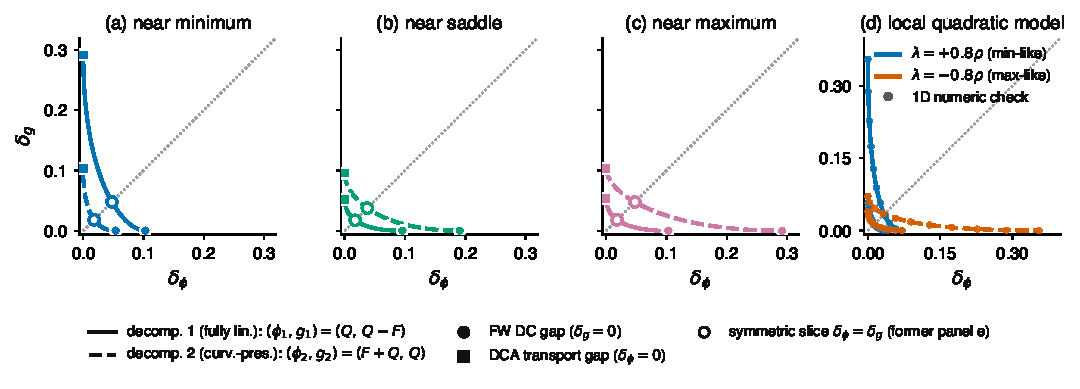
\includegraphics[width=\textwidth]{pareto_frontier_decomposition.pdf}
    \caption{Decomposition dependence read on the $(\delta_\phi,\delta_g)$
    scale, on the example of \citet[Figure~1]{maskan2025}:
    $F(\bx)=\sin(\pi x_1)\cos(\pi x_2)$, $L=\pi^2$, with
    $Q=\frac{L}{2}\|\cdot\|^2$ and the two convex decompositions
    $(\phi_1,g_1)=(Q,\,Q-F)$ (fully linearized, solid) and
    $(\phi_2,g_2)=(F+Q,\,Q)$ (curvature preserving, dashed). A certificate
    $\bv$ lies in $\partial_\delta h(\bar\bx)$ exactly when its Fenchel gap
    $h(\bar\bx)+h^{*}(\bv)-\langle\bv,\bar\bx\rangle\le\delta$; each curve is
    the lower-left (Pareto) boundary of the slack pairs
    $(\delta_\phi,\delta_g)$ for which a \emph{single} certificate $\bv$
    renders $\bar\bx$ a $(\delta_\phi,\delta_g,0)$-critical point of
    $(\phi_i,g_i)$.
    \textbf{a}--\textbf{c}: frontiers at three probe points
    $\bar\bx=\bx^{*}+d\,\bu$ ($d=0.15$, $\bu$ the leading Hessian eigenvector
    of $F$ at the stationary point $\bx^{*}$) near the global minimum, a
    saddle, and the global maximum. On each curve the $\delta_g=0$ intercept
    ($\bullet$) is the Frank--Wolfe DC gap of that decomposition
    (\Cref{lem:gap-dc-slice}), the $\delta_\phi=0$ intercept ($\blacksquare$)
    is the DCA transport gap, and the diagonal $\delta_\phi=\delta_g$ section
    ($\circ$) recovers the symmetric single-dial reading of the mismatch
    $\eps^{*}_{\delta}$. The two decompositions trace genuinely different
    frontiers, and their $\delta_g=0$ intercepts swap order between the
    minimum (curvature preserving smaller) and the maximum (fully linearized
    smaller): the qualitative effect reported by \citet{maskan2025}, localized
    here to an intercept property. Every frontier contracts to the origin as
    $\bar\bx\to\bx^{*}$ at rate $O(d^2)$.
    \textbf{d}: local quadratic model. Along an eigendirection of curvature
    $\lambda$, writing $\rho=L$, the frontiers are
    $\sqrt{2(\rho+\lambda)\delta_\phi}+\sqrt{2\rho\,\delta_g}=|\lambda d|$
    (curvature preserving) and
    $\sqrt{2\rho\,\delta_\phi}+\sqrt{2(\rho-\lambda)\delta_g}=|\lambda d|$
    (fully linearized): moving $F$ across the decomposition transfers the
    curvature coefficient from the $\delta_\phi$ scale to the $\delta_g$
    scale. Dots: matching one-dimensional numeric frontiers on
    $F(t)=\frac{\lambda}{2}t^{2}$. Conjugates of the nonquadratic components
    are evaluated on a grid.}
    \label{fig:decomposition-dependence}
\end{figure}

\Cref{fig:decomposition-dependence} reads the same example on the
$(\delta_\phi,\delta_g)$ scale. At every probe point the two
decompositions trace different Pareto frontiers, yet each is pinned by
the same landmarks: its $\delta_g=0$ intercept is the decomposition's
Frank--Wolfe DC gap and its $\delta_\phi=\delta_g$ section is the
symmetric mismatch reading. The Frank--Wolfe intercepts reproduce the
observation of \citet{maskan2025}---curvature preserving is cheaper near
the minimum and dearer near the maximum---while the whole frontier
shrinks to the origin as $\bar\bx$ approaches the stationary point,
uniformly in the decomposition, in line with
\Cref{prop:vanishing-decomposition-dependence}. In summary, the
trade-off identified by \citet{maskan2025} is real but lives on the
achievability side, namely which certificates a given decomposition
renders cheap to compute. The certificates themselves, expressed in the
$(\delta_\phi,\delta_g,\eps)$ coordinates, subsume the Frank--Wolfe gap
as a $(\delta,0,0)$-slice (\Cref{lem:gap-dc-slice}), transfer without
loss under convex shifts (\Cref{lem:convex-shift-transfer}), and
degrade in a controlled $O(\sqrt{\lambda\delta})$ fashion between
smooth decompositions
(\Cref{prop:vanishing-decomposition-dependence}).


\section{Complexity Analysis of Deterministic DCA}
\label{sec:complexity-analysis-DCA}

This section establishes the iteration complexity of DCA-type methods for
reaching a $(\delta_\phi,\delta_g,\varepsilon)$-critical point of
$F=\phi-g$, without imposing smoothness on $g$. We analyze three
algorithmic templates against this single certificate: (1) exact and inexact
DCA, which solve the strongly convex subproblem to full or controlled accuracy;
(2) proximal DCA, which replaces that solve by a single proximal-subgradient
step; and (3) concave-side smoothing.
% , which, rather than a new method, is
shown to reproduce the same certificate the other two attain. 
% Two devices
% recur throughout, a strong-convexity reformulation that is without loss
% of generality (\Cref{ass:strong-convexity-dc}) and a Fenchel-gap toolkit
% that turns each subproblem's optimality into a transported tolerance. 

\begin{algorithm}[tbp]
    \caption{\textbf{(In)exact DCA}}
    \label{alg: DCA}
    \begin{algorithmic}[1]
        \STATE {\bfseries Input:} Initial point $\bx^0\in\dom \phi $,
        inner solver tolerance $\{\epsilon_k\}_{k=0}^{K-1}$,
        stepsize $\eta$.
        \FOR{$k=0,1,\ldots,K-1$}
            \STATE Compute $\bv^k \in \partial g(\bx^k)$.
            \STATE 
            Solve inner strongly convex subproblem:

            \STATE $\triangleright$ \textbf{Option I:} exact subproblem solve
            \begin{align}
            \label{eq:dca-exact-step}
            \bx^{k+1} = \argmin\limits_{\bx \in \RR^n } \{ \phi (\bx)- \langle \bv^k, \bx \rangle \} 
            \end{align}

            \STATE $\triangleright$ \textbf{Option II:} inexact inner solve
            \begin{align}
            \label{eq:dca-inner-solver-step}
            \bx^{k+1}
            =
            \mathcal S_{\mathcal A_k}(\bx^k,\bv^k;\Theta_k),
            \end{align}
            where $\mathcal S_{\mathcal A_k}$ denotes the inner solver selected
            by $\mathcal A_k$, and $\Theta_k$ collects its parameters and
            stopping tolerance.
        \ENDFOR
        \STATE {\bfseries Output:} $\hat\bx$, chosen uniformly from
        $\{\bx^k\}_{k=0}^{K-1}$.
    \end{algorithmic}
\end{algorithm} 

We use the unified DCA summarized in Algorithm~\ref{alg: DCA}. At the
$k$-th iteration, DCA computes a subgradient $\bv^k \in \partial g(\bx^k)$
and solves a $\gamma$-strongly convex subproblem to obtain $\bx^{k+1}$
(Option I). Option II is an abstract inexact inner-solver interface:
\Cref{alg:inexact-dca-inner} gives one realization, in which the convex
subproblem is solved to value accuracy by an inner first-order method,
and other inner-loop algorithms can be used as long as their output
satisfies the inexact certificate required in the analysis below.

Before analyzing the complexity of DCA, we first introduce the main
assumptions used throughout the section.

\subsection{Main Assumption}
Assume that $F$ is bounded below on $\operatorname{dom}\phi$, and denote
\[
F^\star:=\inf\limits_x F(x)>-\infty,
\qquad
\Delta_0:=F(\bx^0)-F^\star > 0.
\]
For any $\gamma>0$, $F$ admits the reformulation
\[
F = \Big(\phi+\tfrac{\gamma}{2}\|\bx\|^2\Big) - \Big(\tfrac{\gamma}{2}\|\bx\|^2+g\Big),
\]
so WLOG we take $\phi$ and $g$ to be $\gamma$-strongly convex, formalized as follows.

\begin{assumption}
\label{ass:strong-convexity-dc}
The functions $\phi$ and $g$ are strongly convex for some constant
$\gamma>0$, and $g$ has bounded subgradients:
$\sup\limits_{\bx}\sup\limits_{\bv\in\partial g(\bx)}\|\bv\|\le G$.
\end{assumption}

% We also take $\Delta_0>0$ WLOG: if $\Delta_0=0$, then $\bx^0$ is a global
% minimizer of $F$, so for any $\bv\in\partial g(\bx^0)$ and all $\bx$,
% \[
%     \phi(\bx)
%     \;\ge\;
%     g(\bx)+F(\bx^0)
%     \;\ge\;
%     g(\bx^0)+\langle\bv,\bx-\bx^0\rangle+F(\bx^0)
%     \;=\;
%     \phi(\bx^0)+\langle\bv,\bx-\bx^0\rangle,
% \]
% i.e., $\bv\in\partial\phi(\bx^0)\cap\partial g(\bx^0)$, so $\bx^0$ is already
% $(0,0,0)$-critical and the analysis is vacuous.
Our goal is to characterize the iteration complexity of DCA-type methods, without imposing smoothness on $g$, for reaching a $(\delta_\phi,\delta_g,\varepsilon)$-critical
point. As discussed below, the three parameters play distinct roles in this analysis:
$\varepsilon$ controls the residual mismatch between the approximate dual
vectors of $\phi$ and $g$, while $\delta_\phi$ and $\delta_g$ control how
loosely each convex component's Fenchel--Young gap is allowed to vanish.

\subsection{Common Auxiliary Lemmas}
% In particular, $\delta_\phi$ coincides with the primal optimality gap of the
% convex subproblem solved at each DCA iteration,
% \[
%     \min\limits_{\bx}\ \phi(\bx)-\langle \bv^k,\bx\rangle,
% \]
% evaluated at the returned iterate $\bx^{k+1}$. If the subproblem is solved to
% global optimality (an exact oracle), then $\Phi_\phi(\bx^{k+1},\bv^k)=0$,
% i.e., $\delta_\phi=0$; if it is solved only approximately -- e.g., by a fixed
% budget of inner first-order steps -- then $\delta_\phi>0$, and its magnitude
% is precisely the residual primal gap left by the inner solver. Exact
% subproblem solution therefore recovers the stronger regime $\delta_\phi=0$,
% in which $\delta_g$ remains the only source of inexactness, reflecting its
% structural rather than computational origin.

The next lemma is the pivot of the analysis, which shows that the $\phi$-side Fenchel gap $\Phi_\phi$ is at any candidate point equals the value suboptimality of that
point for the current convex subproblem. Consequently, the parameter
$\delta_\phi$ of \Cref{def:delta-eps-critical} coincides, exactly and
without slack, with the accuracy to which the subproblem is solved.

\begin{lemma}
\label{lem:dca-subproblem-value}
Let \Cref{ass:strong-convexity-dc} hold, $\bar\bx\in\dom\phi$,
$\bv\in\partial g(\bar\bx)$, and define
$P(\bx):=\phi(\bx)-\langle\bv,\bx\rangle$. Then the following statements
hold.
\begin{enumerate}
    \item[(i)] $\inf\limits_{\bx\in\RR^n}P(\bx)\ge
    F^\ast+g(\bar\bx)-\langle\bv,\bar\bx\rangle>-\infty$, and
    $\phi^*(\bv)=-\inf\limits_{\bx\in\RR^n}P(\bx)\in\RR$.
    \item[(ii)] For every $\by\in\dom\phi$, the following holds
    \[
        \Phi_\phi(\by,\bv)
        \;=\;
        P(\by)-\inf\limits_{\bx\in\RR^n}P(\bx).
    \]
    \item[(iii)] For every $\sigma\ge0$ and every $\by\in\dom\phi$, the
    following three statements are equivalent:
    \[
        \text{(a) }P(\by)\le\inf\limits_{\bx\in\RR^n}P(\bx)+\sigma;
        \qquad
        \text{(b) }\Phi_\phi(\by,\bv)\le\sigma;
        \qquad
        \text{(c) }\bv\in\partial_\sigma\phi(\by).
    \]
    In particular, $\by\in\argmin\limits_{\bx\in\RR^n}P(\bx)$ if and only if
    $\bv\in\partial\phi(\by)$.
\end{enumerate}
\end{lemma}

\begin{proof}
(i) Since $\bar\bx\in\dom\phi\subseteq\dom g$ and
$\bv\in\partial g(\bar\bx)$, the subgradient inequality gives
\begin{equation}
    g(\bx)\;\ge\;g(\bar\bx)+\langle\bv,\bx-\bar\bx\rangle
    \qquad\text{for all }\bx\in\RR^n,
    \label{eq:g-subgrad-at-xbar}
\end{equation}
equivalently
$\langle\bv,\bx\rangle\le g(\bx)-g(\bar\bx)+\langle\bv,\bar\bx\rangle$
for all $\bx\in\RR^n$. Hence, for every $\bx\in\dom\phi\subseteq\dom g$,
\[
    P(\bx)
    \;=\;
    \phi(\bx)-\langle\bv,\bx\rangle
    \;\ge\;
    \phi(\bx)-g(\bx)+g(\bar\bx)-\langle\bv,\bar\bx\rangle
    \;=\;
    F(\bx)+g(\bar\bx)-\langle\bv,\bar\bx\rangle
    \;\ge\;
    F^\ast+g(\bar\bx)-\langle\bv,\bar\bx\rangle,
\]
while $P(\bx)=+\infty$ for $\bx\notin\dom\phi$. Since $g(\bar\bx)\in\RR$,
the claimed lower bound follows, and it is finite. Furthermore,
$P(\bar\bx)=\phi(\bar\bx)-\langle\bv,\bar\bx\rangle<+\infty$, so
$\inf\limits P\in\RR$. By the definition of the Fenchel conjugate,
\[
    \phi^*(\bv)
    \;=\;
    \sup\limits_{\bx\in\RR^n}\bigl\{\langle\bv,\bx\rangle-\phi(\bx)\bigr\}
    \;=\;
    -\inf\limits_{\bx\in\RR^n}\bigl\{\phi(\bx)-\langle\bv,\bx\rangle\bigr\}
    \;=\;
    -\inf\limits_{\bx\in\RR^n}P(\bx)\;\in\;\RR .
\]

(ii) For $\by\in\dom\phi$, using (i),
\[
    \Phi_\phi(\by,\bv)
    \;=\;
    \phi(\by)+\phi^*(\bv)-\langle\bv,\by\rangle
    \;=\;
    P(\by)+\phi^*(\bv)
    \;=\;
    P(\by)-\inf\limits_{\bx\in\RR^n}P(\bx).
\]

(iii) The equivalence of (a) and (b) is immediate from (ii). The
equivalence of (b) and (c) is \Cref{lem:fenchel-gap-toolkit} applied to
$h=\phi$. The final claim is the case $\sigma=0$.
\end{proof}


The following identity decomposes the per-iteration decrease of $F$
into three nonnegative quantities that together constitute a
$(\delta_\phi,\delta_g,\eps)$-point. It holds for an arbitrary
candidate $\bx^{k+1}$, regardless of how it is produced, and therefore
serves as the common engine underlying both the exact and the
inexact analyses.

\begin{lemma}[One-step decomposition identity]
\label{lem:dca-one-step-identity}
Suppose \Cref{ass:strong-convexity-dc} holds. For any
$\bx^k,\bx^{k+1}\in\dom\phi$ and any $\bv^k\in\partial g(\bx^k)$, it holds that
\begin{equation}
    F(\bx^{k+1})-F(\bx^k)
    \;=\;
    \Phi_\phi(\bx^{k+1},\bv^k)
    \;-\;
    \Phi_\phi(\bx^k,\bv^k)
    \;-\;
    \Phi_g(\bx^{k+1},\bv^k).
    \label{eq:dca-one-step-identity}
\end{equation}
% where
% \[
%     \Phi_\phi(\bx^k,\bv^k)\ge0,
%     \qquad
%     \Phi_\phi(\bx^{k+1},\bv^k)\ge0,
%     \qquad
%     \Phi_g(\bx^{k+1},\bv^k)\ge0.
% \]
\end{lemma}

\begin{proof}
By the Fenchel--Young equality, i.e.,  for any 
\begin{equation}
    g^*(\bv^k)
    \;=\;
    \langle\bv^k,\bx^k\rangle-g(\bx^k)
    \;\in\;\RR,
    \label{eq:fenchel-young-equality-g}
\end{equation} and 
ssubstituting \eqref{eq:fenchel-young-equality-g} into the definition of
$\Phi_g$ gives
\begin{equation}
    \Phi_g(\bx^{k+1},\bv^k)
    \;=\;
    g(\bx^{k+1})+g^*(\bv^k)-\langle\bv^k,\bx^{k+1}\rangle
    \;=\;
    g(\bx^{k+1})-g(\bx^k)-\langle\bv^k,\bx^{k+1}-\bx^k\rangle.
    \label{eq:g-gap-bregman-form}
\end{equation}

On the other hand, rearranging the terms in the definition of
$\Phi_\phi$ yields
\[
    \Phi_\phi(\bx^k,\bv^k)-\Phi_\phi(\bx^{k+1},\bv^k)
    \;=\;
    \bigl[\phi(\bx^k)-\langle\bv^k,\bx^k\rangle\bigr]
    -\bigl[\phi(\bx^{k+1})-\langle\bv^k,\bx^{k+1}\rangle\bigr].
\]

Adding \eqref{eq:g-gap-bregman-form} to the above equality yields
\[
    \Phi_\phi(\bx^k,\bv^k)-\Phi_\phi(\bx^{k+1},\bv^k)
    +\Phi_g(\bx^{k+1},\bv^k)
    \;=\;
    \bigl[\phi(\bx^k)-g(\bx^k)\bigr]
    -\bigl[\phi(\bx^{k+1})-g(\bx^{k+1})\bigr]
    \;=\;
    F(\bx^k)-F(\bx^{k+1}),
\]
which completes the proof.
\end{proof}
By
\Cref{lem:dca-subproblem-value}\,(ii)--(iii), the quantity
$\Phi_\phi(\bx^{k+1},\bv^k)$ is the value inaccuracy of the subproblem
solve and populates the $\delta_\phi$-slot of the certificate at
$\bx^{k+1}$; the quantity $\Phi_g(\bx^{k+1},\bv^k)$ populates the
$\delta_g$-slot at $\bx^{k+1}$; and the quantity $\Phi_\phi(\bx^k,\bv^k)$
populates the $\delta_\phi$-slot of a second certificate anchored at
$\bx^k$, where the $g$-side is exact because $\Phi_g(\bx^k,\bv^k)=0$. The
objective decrease per iteration equals the sum of the two certificate
budgets minus the injected inexactness. In the exact regime the injected
inexactness vanishes and the identity strengthens the classical monotone
descent property of DCA \citep{lethi2009dc,abbaszadehpeivasti2023rate}
into an exact accounting of where the descent goes.

\subsection{Iteration Complexity of DCA-type Methods}
We translate the one-step identity above into finite-time complexity
bounds. We first treat exact DCA, where each convex subproblem is solved
exactly. We then analyze inexact DCA by separating the outer certificate
bound from the inner first-order cost.

\paragraph{Complexity analysis of Exact DCA.} We first analyze the complexity of DCA in \Cref{alg: DCA} with \emph{Option I}, meaning that each subproblem is solved exactly. By \Cref{lem:dca-subproblem-value}\,(ii)--(iii), the update
\eqref{eq:dca-exact-step} is equivalent to
\begin{equation}
    \Phi_\phi(\bx^{k+1},\bv^k)=0,
    \qquad\text{that is,}\qquad
    \bv^k\in\partial\phi(\bx^{k+1}).
    \label{eq:dca-exact-optimality}
\end{equation}

\begin{theorem}[Iteration Complexity of Exact DCA]
\label{thm:dca-exact-complexity}
Suppose \Cref{ass:strong-convexity-dc} holds. Let $\bx^0\in\dom\phi$ and
$\{\bx^k\}_{k\ge0}$ be generated by \Cref{alg: DCA} with \emph{Option I}.
Given $\delta_g>0$, DCA returns a point $\bar{\bx}\in\{\bx^1,\ldots,\bx^K\}$
satisfying $(0,\delta_g,0)$-critical within
$K=\mathcal O(\Delta_0 \delta_g^{-1})$ iterations.
\end{theorem}

\begin{proof}
Substituting the exact optimality condition~\eqref{eq:dca-exact-optimality}
into the one-step identity~\eqref{eq:dca-one-step-identity} gives, for
every $k\ge0$,
\begin{equation}
    F(\bx^k)-F(\bx^{k+1})
    \;=\;
    \Phi_\phi(\bx^k,\bv^k)+\Phi_g(\bx^{k+1},\bv^k)
    \;\ge\;0,
    \label{eq:dca-exact-descent}
\end{equation}
Summing~\eqref{eq:dca-exact-descent} over $k=0,\ldots,K-1$
and using $F(\bx^K)\ge F^\star$, we obtain
\[
    \frac1K\sum_{k=0}^{K-1}
    \Bigl[
        \Phi_\phi(\bx^k,\bv^k)+\Phi_g(\bx^{k+1},\bv^k)
    \Bigr]
    \;\le\;
    \frac{\Delta_0}{K}.
\] where defining
\[
    k^*:=\argmin_{0\le k\le K-1}
    \Bigl[
        \Phi_\phi(\bx^k,\bv^k)+\Phi_g(\bx^{k+1},\bv^k)
    \Bigr]
\]
yields
\[
    \Phi_\phi(\bx^{k^*},\bv^{k^*})+\Phi_g(\bx^{k^*+1},\bv^{k^*})
    \;\le\;\frac{\Delta_0}{K}.
\]
Because both summands are nonnegative, each is individually bounded by
their sum, implying
\begin{equation}
    \Phi_g(\bx^{k^*+1},\bv^{k^*})\;\le\;\frac{\Delta_0}{K}.
    \label{eq:dca-exact-individual-bound}
\end{equation}
Then, we set $\bu=\bv:=\bv^{k^*}$. Combining
\eqref{eq:dca-exact-optimality} with the optimality condition that $\bv^{k^*}\in\partial\phi(\bx^{k^*+1})\cap\partial g(\bx^k)$, we obtain $\bu\in\partial\phi(\bx^{k^*+1})$. By
\eqref{eq:dca-exact-individual-bound} together with
\Cref{lem:fenchel-gap-toolkit}, $\bv\in\partial_{\Delta_0/K}g(\bx^{k^*+1})$.
Hence the following holds
\[
    \operatorname{dist}
    \Bigl(
        \partial_{0}\phi(\bx^{k^*+1}),\,
        \partial_{\Delta_0/K}\,g(\bx^{k^*+1})
    \Bigr)
    \;\le\;
    \|\bu-\bv\|
    \;=\;
    0,
\] i.e., $\bx^{k^*+1}$ is $(0,\Delta_0/K,0)$-critical. Choosing $K=\lceil\Delta_0/\delta_g\rceil$ gives $\Delta_0/K\le\delta_g$.
Taking $\bar\bx:=\bx^{k^*+1}$ completes the proof.
\end{proof}

\blue{
\begin{remark}[Tightness under smooth oracle]
\label{rem:tightness-dimension}
\begin{itemize}
    \item \emph{Matching lower bound.} The rate of
    \Cref{thm:dca-exact-complexity} is tight up to the condition number
    $L/\gamma$: embedding the smooth hard instance of
    \citet{carmon2020lower} as the DC pair
    $\phi=\hat F+\tfrac{L}{2}\|\cdot\|^2$ and
    $g=\tfrac{L}{2}\|\cdot\|^2$ renders the component-wise DC oracle
    informationally equivalent to a standard first-order oracle, and
    yields a lower bound of
    $\Omega(\gamma L^{-1}\Delta\delta^{-1})$ oracle calls for reaching a
    $(0,\delta_g,\varepsilon)$-critical point with 
    $\delta_g=O(\gamma\varepsilon^2/L^2)$;  see \Cref{Appendix: lower bound of DCA}.

    % \item \emph{Dimension.} The embedded instance inherits the zero-chain
    % dimension $d=\Theta(\Delta L\varepsilon^{-2})$ of
    % \citet{carmon2020lower}; the bound itself is dimension-free. In
    % contrast, the one-dimensional barrier construction of
    % \Cref{thm:dc-oracle-limitation-sketch} trades dimension for component
    % growth $G_K=O(KL)$.

    \item \emph{Relation to classical measures.} When $g$ is
    $L_g$-smooth, $\delta_g$ and the same-point residual $\varepsilon$
    are explicitly inter-convertible with constant $L_g^2/\gamma$, so
    $O(\Delta\delta^{-1})$ recovers the classical
    $O(\varepsilon^{-2})$ rate; when $g$ is nonsmooth this equivalence
    provably fails, as the classical target is finite-time unattainable
    (\Cref{thm:dc-oracle-limitation-sketch}).
    % see \Cref{rem:smooth-conversion}.
\end{itemize}
\end{remark}}


\paragraph{Complexity Analysis of Inexact DCA} 

\begin{algorithm}[tbp]
    \caption{\textbf{Inexact DCA}}
    \label{alg:inexact-dca-inner}
    \begin{algorithmic}[1]
        \STATE {\bfseries Input:} Starting point $\bx^0\in\dom\phi$,
        tolerances $\{\sigma_k\}_{k\ge0}$.
        \FOR{$k=0,1,2,\ldots$}
            \STATE Choose $\bv^k\in\partial g(\bx^k)$.
            \STATE Define the convex subproblem
            \[
                P_k(\bx):=\phi(\bx)-\langle\bv^k,\bx\rangle .
            \]
            \STATE Starting from $\by^0=\bx^k$, run an inner first-order
            method to find $\by^{J_k}$ satisfying
            \begin{equation}
                P_k(\by^{J_k})
                \le
                \inf_{\bx\in\RR^n}P_k(\bx)+\sigma_k .
                \label{eq:dca-inexact-value-step}
            \end{equation}
            \STATE Set $\bx^{k+1}:=\by^{J_k}$.
        \ENDFOR
        \STATE {\bfseries Output:} $\{\bx^k\}_{k\ge0}$.
    \end{algorithmic}
\end{algorithm}

We now analyze the complexity of DCA with inexact subproblem solves, as
formalized in \Cref{alg:inexact-dca-inner}. This setting models the
practical situation in which the convex subproblem is solved by an
iterative method and terminated early \citep{yao2022large}. When
$\sigma_k=0$, condition \eqref{eq:dca-inexact-value-step} reduces to
\eqref{eq:dca-exact-step}.

\begin{lemma}
\label{lem:dca-inexact-complexity}
Suppose \Cref{ass:strong-convexity-dc} holds. Let
$\{\bx^k\}_{k\ge0}$ be generated by DCA with tolerances
$\{\sigma_k\}_{k\ge0}\subset[0,+\infty)$. Then the following statements
hold.
\begin{enumerate}
    \item[(i)] For every $k\ge0$, it holds that
    \[
        \Phi_\phi(\bx^{k+1},\bv^k)\;\le\;\sigma_k,
        \qquad\text{equivalently,}\qquad
        \bv^k\in\partial_{\sigma_k}\phi(\bx^{k+1}).
    \]
    \item[(ii)] For every integer $K\ge1$, it holds that
    \begin{equation}
        \sum_{k=0}^{K-1}
        \Bigl[
            \Phi_\phi(\bx^k,\bv^k)
            +\Phi_g(\bx^{k+1},\bv^k)
        \Bigr]
        \;\le\;
        \Delta_0+\sum_{k=0}^{K-1}\sigma_k .
        \label{eq:dca-inexact-telescope}
    \end{equation} Moreover, if  $\sigma_k\equiv\sigma\ge0$ for all $k$, then there exists $k^*\in\{0,1,\ldots,K-1\}$ such that
    \begin{equation}
        \Phi_\phi(\bx^{k^*},\bv^{k^*})
        +\Phi_g(\bx^{k^*+1},\bv^{k^*})
        \;\le\;
        \frac{\Delta_0}{K}+\sigma,
        \label{eq:dca-inexact-best-index}
    \end{equation} i.e.,  $\bx^{k^*+1}$ is a
        $\bigl(\sigma,\ \Delta_0/K+\sigma,\ 0\bigr)$-critical point.
\end{enumerate}
\end{lemma}

\begin{proof}
(i) Fix $k\ge0$. By \Cref{alg:inexact-dca-inner}, the iterate
$\bx^{k+1}$ satisfies the value-inexactness condition
\eqref{eq:dca-inexact-value-step} for the subproblem
$P_k(\bx)=\phi(\bx)-\langle\bv^k,\bx\rangle$. Applying
\Cref{lem:dca-subproblem-value}\,(iii) with
$\bar\bx=\bx^k$, $\bv=\bv^k$, $\by=\bx^{k+1}$, and
$\sigma=\sigma_k$ gives
\[
    \Phi_\phi(\bx^{k+1},\bv^k)\le\sigma_k
    \qquad\Longleftrightarrow\qquad
    \bv^k\in\partial_{\sigma_k}\phi(\bx^{k+1}).
\]
This proves (i).

(ii) Substituting the bound in (i) into the one-step identity
\eqref{eq:dca-one-step-identity} yields, for every $k\ge0$,
\begin{equation}
    F(\bx^k)-F(\bx^{k+1})
    \;=\;
    \Phi_\phi(\bx^k,\bv^k)
    -\Phi_\phi(\bx^{k+1},\bv^k)
    +\Phi_g(\bx^{k+1},\bv^k)
    \;\ge\;
    \Phi_\phi(\bx^k,\bv^k)
    +\Phi_g(\bx^{k+1},\bv^k)
    -\sigma_k .
    \label{eq:dca-inexact-descent}
\end{equation}
Summing~\eqref{eq:dca-inexact-descent} over $k=0,\ldots,K-1$
and using $F(\bx^K)\ge F^\star$, we obtain
\[
    \sum_{k=0}^{K-1}
    \Bigl[
        \Phi_\phi(\bx^k,\bv^k)+\Phi_g(\bx^{k+1},\bv^k)
    \Bigr]
    \;\le\;
    F(\bx^0)-F(\bx^K)+\sum_{k=0}^{K-1}\sigma_k
    \;\le\;
    \Delta_0+\sum_{k=0}^{K-1}\sigma_k,
\]
which proves \eqref{eq:dca-inexact-telescope}.

If $\sigma_k\equiv\sigma$, then the right-hand side of
\eqref{eq:dca-inexact-telescope} equals $\Delta_0+K\sigma$. Define
\[
    k^*
    :=
    \argmin_{0\le k\le K-1}
    \Bigl[
        \Phi_\phi(\bx^k,\bv^k)+\Phi_g(\bx^{k+1},\bv^k)
    \Bigr].
\]
Then
\[
    \Phi_\phi(\bx^{k^*},\bv^{k^*})
    +\Phi_g(\bx^{k^*+1},\bv^{k^*})
    \;\le\;
    \frac{\Delta_0}{K}+\sigma,
\]
which is \eqref{eq:dca-inexact-best-index}. Since
$\Phi_\phi(\bx^{k^*},\bv^{k^*})\ge0$, the same bound gives
\[
    \Phi_g(\bx^{k^*+1},\bv^{k^*})
    \;\le\;
    \frac{\Delta_0}{K}+\sigma .
\]
Part (i) gives
$\bv^{k^*}\in\partial_\sigma\phi(\bx^{k^*+1})$, while
\Cref{lem:fenchel-gap-toolkit} gives
\[
    \bv^{k^*}\in
    \partial_{\Delta_0/K+\sigma}g(\bx^{k^*+1}).
\]
Taking $\bu=\bv=\bv^{k^*}$, we obtain
\[
    \operatorname{dist}
    \Bigl(
        \partial_{\sigma}\phi(\bx^{k^*+1}),\,
        \partial_{\Delta_0/K+\sigma}g(\bx^{k^*+1})
    \Bigr)
    \;\le\;
    \|\bu-\bv\|
    \;=\;
    0.
\]
Hence $\bx^{k^*+1}$ is
$\bigl(\sigma,\Delta_0/K+\sigma,0\bigr)$-critical, completing the proof.
\end{proof}

\begin{theorem}[First-order Complexity of Inexact DCA]
\label{cor:dca-inexact-target}
Suppose \Cref{ass:strong-convexity-dc} holds. Let
$\{\bx^k\}_{k\ge0}$ be generated by \Cref{alg:inexact-dca-inner} with the
constant tolerance
\[
    \sigma_k\equiv\sigma_\star
    :=
    \min\{\delta_\phi,\theta\delta_g\},
    \qquad
    \theta\in(0,1),
\]
where $\delta_\phi,\delta_g>0$. Then DCA returns a
$(\delta_\phi,\delta_g,0)$-critical point
$\bar\bx\in\{\bx^1,\ldots,\bx^K\}$ within $K = \left(\Delta_0(\delta_g-\sigma_\star)^{-1}\right)$ outer iterations. Moreover, if each inner subproblem can be solved to value accuracy
$\sigma_\star$ using at most $\mathcal N_{\rm in}(\sigma_\star)$
inner first-order oracle calls, then the total number of 
first-order oracle calls is at most $ \left(\Delta_0(\delta_g-\sigma_\star)^{-1}  \mathcal N_{\rm in}(\sigma_\star) \right)$.
\end{theorem}

\begin{proof}
Applying \Cref{lem:dca-inexact-complexity}\,(ii) with
$\sigma=\sigma_\star$ gives an index $k^*\in\{0,\ldots,K-1\}$ such that
$\bx^{k^*+1}$ is
$\bigl(\sigma_\star,\Delta_0/K+\sigma_\star,0\bigr)$-critical. Since
$\sigma_\star\le\delta_\phi$ and
$K\ge\Delta_0/(\delta_g-\sigma_\star)$, we have
$\Delta_0/K+\sigma_\star\le\delta_g$. Hence
$\bx^{k^*+1}$ is $(\delta_\phi,\delta_g,0)$-critical. The oracle bound
follows by multiplying the number of outer iterations by the worst-case
inner cost per subproblem.
\end{proof}

\begin{remark}
\label{rem:dca-inexact-total-complexity}
We now specialize the total first-order complexity bound in
\Cref{cor:dca-inexact-target} by instantiating the inexact inner solver
with several standard first-order methods:
\[
\begin{array}{c|c|c}
\text{subproblem structure}
& \mathcal N_{\rm in}(\sigma_\star)
& \text{total first-order complexity}
\\ \hline
\text{convex, subgradient}
& O(\sigma_\star^{-2})
& O\!\left(\dfrac{\Delta_0}{\delta_g}\,\sigma_\star^{-2}\right)
\\
\text{strongly convex, subgradient}
& O(\gamma^{-1}\sigma_\star^{-1})
& O\!\left(\dfrac{\Delta_0}{\delta_g}\,\gamma^{-1}\sigma_\star^{-1}\right)
\\
\text{smooth strongly convex, GD}
& O(\kappa\log(1/\sigma_\star))
& O\!\left(\dfrac{\Delta_0}{\delta_g}\,\kappa\log(1/\sigma_\star)\right)
\\
\text{smooth strongly convex, APG}
& O(\sqrt{\kappa}\log(1/\sigma_\star))
& O\!\left(\dfrac{\Delta_0}{\delta_g}\,\sqrt{\kappa}\log(1/\sigma_\star)\right)
\end{array}
\]
The inner-solver bounds in the second column are the classical
deterministic first-order complexity estimates for subgradient, gradient,
and accelerated gradient methods; see, e.g.,
\citet[Chs.~3--4]{nesterov2018lectures} and
\citet[Chs.~3--5]{beck2017first}.
Here $\gamma$ is the strong convexity modulus of the subproblem $P_k$,
$\kappa=L_P/\gamma$ is its condition number when $P_k$ is $L_P$-smooth,
and the subgradient rows additionally assume the usual bounded-subgradient
constants, absorbed into $O(\cdot)$.

We highlight the insight of this result about the structural and
computational contributions to the total oracle complexity:
\blue{the outer factor $O(\Delta_0/\delta_g)$ is invariant under any
choice of inner solver, while the structure of the subproblem affects
only the multiplicative inner factor, which improves from
$O(\sigma_\star^{-2})$ to $O(\sqrt\kappa\log(1/\sigma_\star))$.}
\blue{Taking $\delta_\phi\to0$, so that $\mathcal N_{\rm in}(\sigma_\star)$
diverges, leaves the outer factor unchanged: even an exact subproblem
solver only certifies a $(0,\delta_g,0)$-critical point; see \Cref{thm:dca-exact-complexity}. This residual
$\delta_g$ therefore originates from the DCA mechanism
itself, namely the mismatch between the subgradient
$\bv^k\in\partial g(\bx^k)$ fixed at the old iterate and the certificate
evaluated at the new iterate $\bx^{k+1}$, rather than from any deficiency
of the inner solver.} This reflects, at the level of oracle complexity,
the asymmetry of \Cref{def:delta-eps-critical}: $\delta_g$ is a
structural cost of the nonsmooth component $g$, whereas $\delta_\phi$ is
a computational cost that enters only through $\mathcal N_{\rm in}$.
\blue{This decomposition constitutes an algorithmic rationale for
adopting two-sided tolerances in \Cref{def:delta-eps-critical}: merging
$\delta_\phi$ and $\delta_g$ into a single parameter forces the inner
accuracy to match the outer structural tolerance, eliminating the
freedom to decouple the two costs that the schedule
$\sigma_k\equiv\sigma_\star=\min\{\delta_\phi,\theta\delta_g\}$ in
\Cref{cor:dca-inexact-target} exploits. We emphasize that this invariance
is established within the DCA linearization framework and the two-point
certificate structure of \Cref{def:delta-eps-critical}; whether it
persists as a lower bound over a broader class of first-order algorithms
for Problem~\eqref{prob:main} is left open.}
\end{remark}

\subsection{Iteration Complexity of Proximal DCA-type Methods}
\label{subsec:prox-subgrad-dca}
We now analyze proximal DCA-type updates. A proximal term shifts the
$\phi$-side certificate from $\bv^k$ to a transported vector of the
form $\bu^{k+1}=\bv^k-\gamma^{-1}(\bx^{k+1}-\bx^k)$; the resulting
step-proportional residual $r\|\bx^{k+1}-\bx^k\|$ is what activates the
mismatch slot $\eps$, whereas bare DCA, which has no proximal term,
produces no shift and activates only the Fenchel-gap slots
$\delta_\phi,\delta_g$. The two deterministic updates---the single-loop
proximal-subgradient DCA (\Cref{alg:ps-dca}) and the exact proximal DCA
as its special case---share this mechanism exactly, so we isolate their
common estimates as \Cref{cond:certified-prox-descent}, prove the
complexity bound once at that level, and then verify the condition for
each. The stochastic variant of PS-DCA follows the same template but
adds a first-order gradient-error term to the residual; it is treated
separately in \Cref{subsec:stoch-ps-dca}.
Throughout this subsection, for
$\bv^k\in\partial g(\bx^k)$ and $s^k:=\bx^{k+1}-\bx^k$, define the
transported Fenchel gap of $g$
\begin{equation}
    \delta_g^{k+1}
    :=
    \Phi_g(\bx^{k+1},\bv^k)
    =
    g(\bx^{k+1})-g(\bx^k)
    -\langle \bv^k,\bx^{k+1}-\bx^k\rangle .
    \label{eq:prox-dca-transport-g-gap}
\end{equation}
The equality uses $\bv^k\in\partial g(\bx^k)$ and the Fenchel--Young
identity. In particular,
\[
    \bv^k\in\partial_{\delta_g^{k+1}} g(\bx^{k+1})
\]
by \Cref{lem:fenchel-gap-toolkit}: the subgradient $\bv^k$ that is exact
at $\bx^k$ becomes a $\delta_g^{k+1}$-subgradient once transported to
$\bx^{k+1}$.

\begin{condition}
\label{cond:certified-prox-descent}
Given $\bx^0\in\dom\phi$ and constants $a>0$, $r>0$, the sequences
$\{\bx^{k+1}\}$ and $\{\bu^{k+1}\}$, together with a choice
$\bv^k\in\partial g(\bx^k)$, satisfy the following: for every $k$ there
exists $\sigma_k\ge0$ such that the $\phi$-side
certificate
\begin{align}
    \bu^{k+1}
    &\in
    \partial_{\sigma_k}\phi(\bx^{k+1}),
    \label{eq:abstract-prox-phi-cert}
    \\
    \|\bu^{k+1}-\bv^k\|
    &\le
    r\|\bx^{k+1}-\bx^k\|,
    \label{eq:abstract-prox-dual-residual}
\end{align}
and the descent estimate
\begin{equation}
    F(\bx^k)-F(\bx^{k+1})
    \ge
    \delta_g^{k+1}
    +a\|\bx^{k+1}-\bx^k\|^2
    -\sigma_k
    \label{eq:abstract-prox-descent}
\end{equation}
hold.
\end{condition}

The next lemma is the abstract accounting device behind the
deterministic results in this subsection. It separates the two effects
in the certificate: the $\phi$-side Fenchel tolerance and the
transported $g$-side Fenchel tolerance.

\begin{lemma}
\label{lem:abstract-prox-certificate-bound}
Suppose $F^\star>-\infty$ and let $\Delta_0:=F(\bx^0)-F^\star$. Let
$K\ge1$, and suppose \Cref{cond:certified-prox-descent} holds for
$k=0,\ldots,K-1$ with
\[
    0\le\sigma_k\le\bar\sigma .
\]
Define
\[
    \hat k
    \in
    \argmin_{0\le k\le K-1}
    \bigl\{
        \delta_g^{k+1}
        +a\|\bx^{k+1}-\bx^k\|^2
    \bigr\},
    \qquad
    \bar\bx:=\bx^{\hat k+1}.
\]
Then $\bar\bx$ satisfies
\begin{align}
    \delta_g^{\hat k+1}
    &\le
    \frac{\Delta_0}{K}+\bar\sigma,
    \label{eq:abstract-prox-deltag-bound}
    \\
    \|\bx^{\hat k+1}-\bx^{\hat k}\|
    &\le
    \sqrt{
        \frac{1}{a}
        \left(
            \frac{\Delta_0}{K}+\bar\sigma
        \right)
    },
    \label{eq:abstract-prox-step-bound}
\end{align}
and hence
\begin{equation}
    \operatorname{dist}
    \left(
        \partial_{\bar\sigma}\phi(\bar\bx),
        \partial_{\frac{\Delta_0}{K}+\bar\sigma}g(\bar\bx)
    \right)
    \le
    r
    \sqrt{
        \frac{1}{a}
        \left(
            \frac{\Delta_0}{K}+\bar\sigma
        \right)
    } .
    \label{eq:abstract-prox-critical-bound}
\end{equation}
Consequently, $\bar\bx$ is a
\[
    \left(
        \bar\sigma,\,
        \frac{\Delta_0}{K}+\bar\sigma,\,
        r
        \sqrt{
            \frac{1}{a}
            \left(
                \frac{\Delta_0}{K}+\bar\sigma
            \right)
        }
    \right)\text{-critical point}.
\]
\end{lemma}

\begin{proof}
Summing the descent estimate \eqref{eq:abstract-prox-descent} over
$k=0,\ldots,K-1$ gives
\[
    \sum_{k=0}^{K-1}
    \left[
        \delta_g^{k+1}
        +
        a\|\bx^{k+1}-\bx^k\|^2
    \right]
    \le
    F(\bx^0)-F(\bx^K)+\sum_{k=0}^{K-1}\sigma_k .
\]
Since $F(\bx^K)\ge F^\star$ and $\sigma_k\le\bar\sigma$, we obtain
\begin{equation}
    \sum_{k=0}^{K-1}
    \left[
        \delta_g^{k+1}
        +
        a\|\bx^{k+1}-\bx^k\|^2
    \right]
    \le
    \Delta_0+K\bar\sigma .
    \label{eq:abstract-prox-telescope}
\end{equation}
By the definition of $\hat k$,
\[
    \delta_g^{\hat k+1}
    +
    a\|\bx^{\hat k+1}-\bx^{\hat k}\|^2
    \le
    \frac{\Delta_0}{K}+\bar\sigma .
\]
Both terms on the left-hand side are nonnegative, and hence
\eqref{eq:abstract-prox-deltag-bound} and
\eqref{eq:abstract-prox-step-bound} follow.

It remains to verify the same-point certificate. By
\eqref{eq:abstract-prox-phi-cert} and $\sigma_{\hat k}\le\bar\sigma$,
\[
    \bu^{\hat k+1}
    \in
    \partial_{\sigma_{\hat k}}\phi(\bx^{\hat k+1})
    \subseteq
    \partial_{\bar\sigma}\phi(\bx^{\hat k+1}).
\]
By the definition of $\delta_g^{\hat k+1}$ and
\eqref{eq:abstract-prox-deltag-bound},
\[
    \bv^{\hat k}
    \in
    \partial_{\delta_g^{\hat k+1}}g(\bx^{\hat k+1})
    \subseteq
    \partial_{\frac{\Delta_0}{K}+\bar\sigma}g(\bx^{\hat k+1}).
\]
Therefore
\[
\begin{aligned}
    \operatorname{dist}
    \left(
        \partial_{\bar\sigma}\phi(\bx^{\hat k+1}),
        \partial_{\frac{\Delta_0}{K}+\bar\sigma}g(\bx^{\hat k+1})
    \right)
    &\le
    \|\bu^{\hat k+1}-\bv^{\hat k}\|
    \\
    &\le
    r\|\bx^{\hat k+1}-\bx^{\hat k}\| .
\end{aligned}
\]
Combining this inequality with \eqref{eq:abstract-prox-step-bound}
proves \eqref{eq:abstract-prox-critical-bound}.
\end{proof}

The selection of $\hat k$ uses only computable quantities:
$\delta_g^{k+1}$ is evaluated from function values of $g$ and the
chosen $\bv^k$, and $\|\bx^{k+1}-\bx^k\|$ is observed, so $\hat k$ is
implementable without knowledge of the certificate tolerance
$\sigma_k$.

\begin{theorem}
\label{thm:abstract-prox-target}
Suppose the assumptions of \Cref{lem:abstract-prox-certificate-bound}
hold. Let target tolerances
$\delta_\phi,\delta_g,\eps>0$ be given, and choose
$\bar\sigma$ such that
\begin{equation}
    0\le\bar\sigma\le\delta_\phi,
    \qquad
    \bar\sigma
    <
    \min\left\{
        \delta_g,\,
        \frac{a\eps^2}{r^2}
    \right\}.
    \label{eq:abstract-prox-target-compatibility}
\end{equation}
If
\begin{equation}
    K
    \ge
    \left\lceil
    \Delta_0
    \max\left\{
        \frac{1}{\delta_g-\bar\sigma},\,
        \frac{1}{
            \frac{a\eps^2}{r^2}
            -
            \bar\sigma
        }
    \right\}
    \right\rceil ,
    \label{eq:abstract-prox-target-K}
\end{equation}
then the output $\bar\bx$ of
\Cref{lem:abstract-prox-certificate-bound} is a
$(\delta_\phi,\delta_g,\eps)$-critical point.
\end{theorem}

\begin{proof}
The first lower bound in \eqref{eq:abstract-prox-target-K} gives
\[
    \frac{\Delta_0}{K}+\bar\sigma
    \le
    \delta_g.
\]
The second lower bound gives
\[
    \frac{\Delta_0}{K}+\bar\sigma
    \le
    \frac{a\eps^2}{r^2}.
\]
Substituting these two inequalities into
\eqref{eq:abstract-prox-critical-bound} yields
\[
    \operatorname{dist}
    \left(
        \partial_{\bar\sigma}\phi(\bar\bx),
        \partial_{\delta_g}g(\bar\bx)
    \right)
    \le
    r\sqrt{
        \frac{1}{a}
        \cdot
        \frac{a\eps^2}{r^2}
    }
    =
    \eps .
\]
Finally, $\bar\sigma\le\delta_\phi$ implies
$\partial_{\bar\sigma}\phi(\bar\bx)
\subseteq
\partial_{\delta_\phi}\phi(\bar\bx)$, so $\bar\bx$ is
$(\delta_\phi,\delta_g,\eps)$-critical.
\end{proof}

We now verify \Cref{cond:certified-prox-descent} for concrete updates. We consider the composite case
\begin{equation}
    F(\bx)=f(\bx)+h(\bx)-g(\bx),
    \qquad
    \phi:=f+h,
    \label{eq:composite-ps-dca-model}
\end{equation}
where $f:\RR^n\to\RR$ is convex and $L_f$-smooth, and $h,g$ are
proper closed convex functions. We assume that the proximal mapping of
$h$ is easy to compute. This setting gives a single-loop realization of
the preceding certificate theorem.

\subsubsection{Proximal-Subgradient DCA}


For a stepsize $\eta\in(0,2/L_f)$, the proximal-subgradient DCA
(PS-DCA) update is
\begin{equation}
    \bx^{k+1}
    =
    \prox_{\eta h}
    \left(
        \bx^k-\eta(\nabla f(\bx^k)-\bv^k)
    \right),
    \qquad
    \bv^k\in\partial g(\bx^k).
    \label{eq:ps-dca-step}
\end{equation}
Equivalently,
\[
    \bx^{k+1}
    =
    \argmin_{\bx\in\RR^n}
    \left\{
        h(\bx)
        +
        \langle \nabla f(\bx^k)-\bv^k,\bx\rangle
        +
        \frac{1}{2\eta}\|\bx-\bx^k\|^2
    \right\}.
\]

Define
\[
    a_\eta:=\frac{1}{\eta}-\frac{L_f}{2}>0,
    \qquad
    r_\eta:=\frac{1}{\eta}+L_f .
\]

\begin{algorithm}[tbp]
    \caption{\textbf{Proximal-Subgradient DCA (PS-DCA)}}
    \label{alg:ps-dca}
    \begin{algorithmic}[1]
        \STATE {\bfseries Input:} $\bx^0\in\dom\phi$, stepsize
        $\eta\in(0,2/L_f)$, iteration number $K\ge1$.
        \FOR{$k=0,1,\ldots,K-1$}
            \STATE Choose $\bv^k\in\partial g(\bx^k)$.
            \STATE
            $\bx^{k+1}
            =\prox_{\eta h}
            \bigl(\bx^k-\eta(\nabla f(\bx^k)-\bv^k)\bigr)$.
        \ENDFOR
        \STATE Choose
        $\hat k\in\argmin_{0\le k\le K-1}
        \bigl\{\delta_g^{k+1}+a_\eta\|\bx^{k+1}-\bx^k\|^2\bigr\}$,
        with $\delta_g^{k+1}$ as in
        \eqref{eq:prox-dca-transport-g-gap}.
        \STATE {\bfseries Output:} $\bar\bx=\bx^{\hat k+1}$.
    \end{algorithmic}
\end{algorithm}

\begin{lemma}[PS-DCA realization]
\label{lem:ps-dca-realization}
Assume \eqref{eq:composite-ps-dca-model} and let
$\{\bx^k\}_{k\ge0}$ be generated by \eqref{eq:ps-dca-step}, with
$a_\eta,r_\eta$ defined above. Then \Cref{cond:certified-prox-descent}
holds with
\[
    a=a_\eta,
    \qquad
    r=r_\eta,
    \qquad
    \sigma_k=0 .
\]
More precisely, there exists
$\bu^{k+1}\in\partial\phi(\bx^{k+1})$ such that
\begin{align}
    \|\bu^{k+1}-\bv^k\|
    &\le
    r_\eta\|\bx^{k+1}-\bx^k\|,
    \label{eq:ps-dca-residual}
    \\
    F(\bx^k)-F(\bx^{k+1})
    &\ge
    \delta_g^{k+1}
    +
    a_\eta\|\bx^{k+1}-\bx^k\|^2 .
    \label{eq:ps-dca-descent}
\end{align}
\end{lemma}

\begin{proof}
Let $s^k:=\bx^{k+1}-\bx^k$. The optimality condition of
\eqref{eq:ps-dca-step} gives
\[
    \zero
    \in
    \partial h(\bx^{k+1})
    +
    \nabla f(\bx^k)
    -
    \bv^k
    +
    \frac{1}{\eta}s^k .
\]
Hence there exists $\bw^{k+1}\in\partial h(\bx^{k+1})$ such that
\[
    \bw^{k+1}
    =
    \bv^k
    -
    \nabla f(\bx^k)
    -
    \frac{1}{\eta}s^k .
\]
Since $f$ is convex and differentiable,
\[
    \bu^{k+1}
    :=
    \nabla f(\bx^{k+1})+\bw^{k+1}
    \in
    \partial(f+h)(\bx^{k+1})
    =
    \partial\phi(\bx^{k+1}).
\]
Moreover,
\[
\begin{aligned}
    \|\bu^{k+1}-\bv^k\|
    &=
    \left\|
        \nabla f(\bx^{k+1})-\nabla f(\bx^k)
        -
        \frac{1}{\eta}s^k
    \right\|
    \\
    &\le
    L_f\|s^k\|+\frac{1}{\eta}\|s^k\|
    =
    r_\eta\|s^k\|,
\end{aligned}
\]
which proves \eqref{eq:ps-dca-residual}.

It remains to prove the descent estimate. Define
\[
    Q_k(\bx)
    :=
    h(\bx)
    +
    \langle \nabla f(\bx^k)-\bv^k,\bx\rangle
    +
    \frac{1}{2\eta}\|\bx-\bx^k\|^2 .
\]
The function $Q_k$ is $\eta^{-1}$-strongly convex, and
$\bx^{k+1}$ minimizes $Q_k$. Hence
\[
    Q_k(\bx^k)-Q_k(\bx^{k+1})
    \ge
    \frac{1}{2\eta}\|s^k\|^2.
\]
Expanding this inequality gives
\begin{equation}
    h(\bx^k)-h(\bx^{k+1})
    +
    \langle \bv^k-\nabla f(\bx^k),s^k\rangle
    \ge
    \frac{1}{\eta}\|s^k\|^2 .
    \label{eq:ps-dca-h-descent}
\end{equation}
By $L_f$-smoothness of $f$,
\[
    f(\bx^{k+1})
    \le
    f(\bx^k)
    +
    \langle\nabla f(\bx^k),s^k\rangle
    +
    \frac{L_f}{2}\|s^k\|^2,
\]
or equivalently
\begin{equation}
    f(\bx^k)-f(\bx^{k+1})
    \ge
    -\langle\nabla f(\bx^k),s^k\rangle
    -
    \frac{L_f}{2}\|s^k\|^2 .
    \label{eq:ps-dca-f-descent}
\end{equation}
Combining \eqref{eq:ps-dca-h-descent} and
\eqref{eq:ps-dca-f-descent}, and using
\[
    \delta_g^{k+1}
    =
    g(\bx^{k+1})-g(\bx^k)-\langle\bv^k,s^k\rangle,
\]
we obtain
\[
\begin{aligned}
    F(\bx^k)-F(\bx^{k+1})
    &=
    f(\bx^k)-f(\bx^{k+1})
    +
    h(\bx^k)-h(\bx^{k+1})
    +
    g(\bx^{k+1})-g(\bx^k)
    \\
    &=
    f(\bx^k)-f(\bx^{k+1})
    +
    h(\bx^k)-h(\bx^{k+1})
    +
    \langle\bv^k,s^k\rangle
    +
    \delta_g^{k+1}
    \\
    &\ge
    \left(
        \frac{1}{\eta}
        -
        \frac{L_f}{2}
    \right)
    \|s^k\|^2
    +
    \delta_g^{k+1}.
\end{aligned}
\]
This proves \eqref{eq:ps-dca-descent}.
\end{proof}

\begin{corollary}[Iteration complexity of PS-DCA]
\label{cor:ps-dca-complexity}
Suppose $F^\star>-\infty$ and the assumptions of
\Cref{lem:ps-dca-realization} hold. Let
$\eta\in(0,2/L_f)$ and let $\{\bx^k\}_{k\ge0}$ be generated by
\eqref{eq:ps-dca-step}. Then for every $K\ge1$, there exists
$\hat k\in\{0,\ldots,K-1\}$ such that
$\bar\bx:=\bx^{\hat k+1}$ is a
\begin{equation}
    \left(
        0,\,
        \frac{\Delta_0}{K},\,
        r_\eta
        \sqrt{
            \frac{\Delta_0}{a_\eta K}
        }
    \right)\text{-critical point}.
    \label{eq:ps-dca-rate}
\end{equation}
Consequently, to obtain a $(0,\delta_g,\eps)$-critical point, it
suffices to take
\begin{equation}
    K
    \ge
    \left\lceil
    \max\left\{
        \frac{\Delta_0}{\delta_g},\,
        \frac{r_\eta^2\Delta_0}{a_\eta\eps^2}
    \right\}
    \right\rceil .
    \label{eq:ps-dca-target-K}
\end{equation}
In particular, for the standard choice $\eta=1/L_f$,
\[
    a_\eta=\frac{L_f}{2},
    \qquad
    r_\eta=2L_f,
\]
and \eqref{eq:ps-dca-target-K} becomes
\begin{equation}
    K
    \ge
    \left\lceil
    \max\left\{
        \frac{\Delta_0}{\delta_g},\,
        \frac{8L_f\Delta_0}{\eps^2}
    \right\}
    \right\rceil .
    \label{eq:ps-dca-standard-stepsize-K}
\end{equation}
The constant in the $\eps^{-2}$ term is minimized within the bound
\eqref{eq:ps-dca-target-K} by taking $\eta=1/(2L_f)$, which gives
\[
    \frac{r_\eta^2}{a_\eta}=6L_f .
\]
\end{corollary}

\begin{proof}
Apply \Cref{lem:abstract-prox-certificate-bound} with
$a=a_\eta$, $r=r_\eta$, and $\bar\sigma=0$, using
\Cref{lem:ps-dca-realization}. This gives
\[
    \delta_g^{\hat k+1}\le\frac{\Delta_0}{K},
    \qquad
    \|\bu^{\hat k+1}-\bv^{\hat k}\|
    \le
    r_\eta
    \sqrt{\frac{\Delta_0}{a_\eta K}},
\]
which is exactly \eqref{eq:ps-dca-rate}. The target bound
\eqref{eq:ps-dca-target-K} follows by requiring
$\Delta_0/K\le\delta_g$ and
$r_\eta\sqrt{\Delta_0/(a_\eta K)}\le\eps$.

For $\eta=1/L_f$,
\[
    \frac{r_\eta^2}{a_\eta}
    =
    \frac{(2L_f)^2}{L_f/2}
    =
    8L_f.
\]
For the last claim, set $a=1/\eta$ and minimize
\[
    \frac{(a+L_f)^2}{a-L_f/2}
    \qquad
    \text{over }a>L_f/2.
\]
The derivative vanishes at $a=2L_f$, i.e., at
$\eta=1/(2L_f)$, and the corresponding value is
\[
    \frac{(3L_f)^2}{3L_f/2}=6L_f.
\]
\end{proof}

\subsubsection{Exact Proximal DCA as a Special Case}

The classical exact proximal DCA update with parameter $\gamma>0$,
\begin{equation}
    \bx^{k+1}
    =
    \argmin_{\bx\in\RR^n}
    \left\{
        \phi(\bx)-\langle\bv^k,\bx\rangle
        +
        \frac{1}{2\gamma}\|\bx-\bx^k\|^2
    \right\},
    \qquad
    \bv^k\in\partial g(\bx^k),
    \label{eq:exact-prox-dca-step}
\end{equation}
is the instance of \eqref{eq:ps-dca-step} obtained by taking
$f\equiv0$ and $h=\phi$ with stepsize $\eta=\gamma$: the smooth part
vanishes, so $L_f=0$, every stepsize $\gamma>0$ is admissible, and the
update reduces to
$\bx^{k+1}=\prox_{\gamma\phi}(\bx^k+\gamma\bv^k)$, which is
\eqref{eq:exact-prox-dca-step}. The quadratic term makes the
subproblem strongly convex, so the minimizer is unique whenever
$\phi$ is proper closed convex; computing it is exactly the proximal
oracle for the full convex part $\phi$. \Cref{lem:ps-dca-realization}
applies with $L_f=0$ and yields the realization constants
\[
    a=\frac{1}{\gamma},
    \qquad
    r=\frac{1}{\gamma},
    \qquad
    \sigma_k=0,
\]
with the shifted dual certificate
$\bu^{k+1}=\bv^k-\gamma^{-1}(\bx^{k+1}-\bx^k)\in\partial\phi(\bx^{k+1})$.

\begin{corollary}[Iteration complexity of exact proximal DCA]
\label{cor:exact-prox-dca-complexity}
Suppose $F^\star>-\infty$, let $\phi$ and $g$ be proper closed convex
functions, and let $\{\bx^k\}_{k\ge0}$ be generated by
\eqref{eq:exact-prox-dca-step}. Then for every $K\ge1$, there exists
$\hat k\in\{0,\ldots,K-1\}$ such that
$\bar\bx:=\bx^{\hat k+1}$ is a
\begin{equation}
    \left(
        0,\,
        \frac{\Delta_0}{K},\,
        \sqrt{\frac{\Delta_0}{\gamma K}}
    \right)\text{-critical point}.
    \label{eq:exact-prox-dca-rate}
\end{equation}
Consequently, to obtain a $(0,\delta_g,\eps)$-critical point, it
suffices to take
\begin{equation}
    K
    \ge
    \left\lceil
    \max\left\{
        \frac{\Delta_0}{\delta_g},\,
        \frac{\Delta_0}{\gamma\eps^2}
    \right\}
    \right\rceil .
    \label{eq:exact-prox-dca-target-K}
\end{equation}
In particular, if $K\ge\lceil\Delta_0/(\gamma\eps^2)\rceil$, then the
same output is a $(0,\gamma\eps^2,\eps)$-critical point.
\end{corollary}

\begin{proof}
Apply \Cref{lem:abstract-prox-certificate-bound} with the constants
$a=r=\gamma^{-1}$ and $\bar\sigma=0$ supplied by
\Cref{lem:ps-dca-realization} with $f\equiv0$ and $\eta=\gamma$. Since
$r\sqrt{\Delta_0/(aK)}=\sqrt{\Delta_0/(\gamma K)}$, the abstract bound
\eqref{eq:abstract-prox-critical-bound} gives
\eqref{eq:exact-prox-dca-rate}, and
\eqref{eq:exact-prox-dca-target-K} follows by imposing
$\Delta_0/K\le\delta_g$ and $\sqrt{\Delta_0/(\gamma K)}\le\eps$.
\end{proof}

\begin{remark}[Realizations and activated slots]
\label{rem:prox-realization-table}
The two realizations above fit the same abstract certificate template:
\[
\begin{array}{c|c|c|c|c}
\text{method}
& a
& r
& \delta_\phi\text{-slot}
& \eps\text{-slot}
\\ \hline
\text{exact proximal DCA}
& \gamma^{-1}
& \gamma^{-1}
& 0
& \gamma^{-1}\|\bx^{k+1}-\bx^k\|
\\
\text{PS-DCA for }\phi=f+h
& \eta^{-1}-L_f/2
& \eta^{-1}+L_f
& 0
& (\eta^{-1}+L_f)\|\bx^{k+1}-\bx^k\|
\end{array}
\]
Thus exact proximal DCA and PS-DCA both activate the $\eps$-slot,
whereas classical bare DCA activates only the Fenchel-gap slots
$\delta_\phi,\delta_g$.
\end{remark}

\begin{remark}[Value-gap inexactness for the proximal subproblem]
\label{rem:prox-value-gap-warning}
The parameter $\sigma_k$ in
\eqref{eq:abstract-prox-phi-cert}--\eqref{eq:abstract-prox-descent} is a
certificate/decrease tolerance. A pure value-gap condition for the
proximalized subproblem,
\[
    M_k(\bx^{k+1})\le\inf_{\bx}M_k(\bx)+\sigma_k,
    \qquad
    M_k(\bx):=
    \phi(\bx)-\langle\bv^k,\bx\rangle
    +
    \frac{1}{2\gamma}\|\bx-\bx^k\|^2,
\]
does not by itself imply
\[
    \bv^k-\gamma^{-1}(\bx^{k+1}-\bx^k)
    \in
    \partial_{\sigma_k}\phi(\bx^{k+1}).
\]
Indeed, expanding the value-gap inequality around $\bx^{k+1}$ leaves an
additional term
\[
    -\frac{1}{2\gamma}\|\bz-\bx^{k+1}\|^2
\]
in the supporting inequality for $\phi$, which is unbounded below as a
function of $\bz$. For this reason, the unified theorem is stated in
terms of the verifiable certificate
\eqref{eq:abstract-prox-phi-cert} and the descent estimate
\eqref{eq:abstract-prox-descent}. Exact proximal DCA and PS-DCA satisfy
these conditions with $\sigma_k=0$.
\end{remark}

\begin{remark}[Coupling between $\delta_g$ and $\eps$]
\label{rem:prox-deltag-eps-coupling}
\Cref{cor:exact-prox-dca-complexity} gives the same output point with
\[
    \delta_g
    \le
    \frac{\Delta_0}{K},
    \qquad
    \eps
    \le
    \sqrt{\frac{\Delta_0}{\gamma K}}.
\]
Therefore, choosing $K=\lceil\Delta_0/(\gamma\eps^2)\rceil$ gives
\[
    \delta_g\le\gamma\eps^2.
\]
This is the precise proximal DCA coupling between the transported
Fenchel error and the dual certificate mismatch. It explains why the
proximal analysis is the natural source of an
$O(\Delta_0/(\gamma\eps^2))$ upper bound for the $\eps$-slot, while the
bare DCA analysis gives $\eps=0$ and only measures $\delta_g$.
\end{remark}

\subsection{Smoothing and the Two-Sided Certificate}
\label{sec:smoothing-certificate}

Smoothing the concave part is a third, and popular, route to nonsmooth DC
problems. Rather than propose a new method, we use it to make one point: the
$(\delta_{\phi},\delta_g,\eps)$-criticality of \Cref{def:delta-eps-critical} is
exactly the object such smoothing produces, so existing smoothing guarantees are
\emph{relabelings} of our certificate. Fix $\mu>0$ and recall the Moreau
envelope of $g$,
\begin{equation}
    g_\mu(\bx)
    :=
    \min_{\by\in\RR^n}
    \Bigl\{
        g(\by)+\tfrac{1}{2\mu}\|\by-\bx\|^2
    \Bigr\},
    \qquad
    \tilde{\bx}:=\prox_{\mu g}(\bx)
    =\argmin_{\by\in\RR^n}
    \Bigl\{
        g(\by)+\tfrac{1}{2\mu}\|\by-\bx\|^2
    \Bigr\},
    \label{eq:moreau-envelope}
\end{equation}
where the minimizer $\tilde{\bx}$ is unique because the inner objective is
$\tfrac1\mu$-strongly convex. Throughout this subsection we take
$(\phi,g)\in\mathcal D(\Delta,L,G)$, so both convex components are
finite-valued with uniformly bounded subgradients; accordingly we write
\[
    G_g:=\sup_{\bx}\;\sup_{\bv\in\partial g(\bx)}\|\bv\|\;\le\;G,
    \qquad
    G_\phi:=\sup_{\bx}\;\sup_{\bu\in\partial\phi(\bx)}\|\bu\|\;\le\;G .
\]
Replacing $g$ by $g_\mu$ renders the concave part smooth, and
$\eps$-criticality of the smoothed problem $\phi-g_\mu$ reads
$\operatorname{dist}\bigl(\partial\phi(\bx),\{\nabla g_\mu(\bx)\}\bigr)\le\eps$.
The next lemma shows that this smoothed certificate is, verbatim, a
$(\delta_{\phi},\delta_g,\eps)$-certificate for the original nonsmooth problem,
with an explicit $\delta_g$ that is linear in $\mu$.

\begin{lemma}[One-sided Moreau reduction]
\label{lem:moreau-reduction}
Let $(\phi,g)\in\mathcal D(\Delta,L,G)$, fix $\mu>0$, and suppose
$\bx\in\RR^n$ satisfies the $\eps$-criticality condition for the smoothed
problem $\phi-g_\mu$,
\[
    \operatorname{dist}\bigl(\partial\phi(\bx),\{\nabla g_\mu(\bx)\}\bigr)\le\eps ;
\]
equivalently, there exists $\bu\in\partial\phi(\bx)$ with
$\|\bu-\nabla g_\mu(\bx)\|\le\eps$. Then $\bx$ is a
$\bigl(0,\,2G_g^2\mu,\,\eps\bigr)$-critical point of the original problem
\eqref{prob:main} in the sense of
\Cref{def:delta-eps-critical}.
\end{lemma}

\begin{proof}
Write $\bv:=\nabla g_\mu(\bx)$ and $\tilde{\bx}:=\prox_{\mu g}(\bx)$.

\emph{Step 1 (Moreau identities).}
The optimality condition for $\tilde{\bx}$ in \eqref{eq:moreau-envelope} is
$\zero\in\partial g(\tilde{\bx})+\tfrac1\mu(\tilde{\bx}-\bx)$, hence
\begin{equation}
    \bv=\nabla g_\mu(\bx)=\frac{\bx-\tilde{\bx}}{\mu}\in\partial g(\tilde{\bx}).
    \label{eq:moreau-grad}
\end{equation}
Since $\bv\in\partial g(\tilde{\bx})$ and the subgradients of $g$ are bounded by
$G_g$, taking norms in \eqref{eq:moreau-grad} gives
\begin{equation}
    \|\bx-\tilde{\bx}\|=\mu\|\bv\|\le\mu G_g .
    \label{eq:prox-move}
\end{equation}

\emph{Step 2 (Transported Fenchel gap).}
Because $\bv\in\partial g(\tilde{\bx})$, the Fenchel--Young equality of
\Cref{lem:fenchel-gap-toolkit} at $\tilde{\bx}$ yields
$g^*(\bv)=\langle\bv,\tilde{\bx}\rangle-g(\tilde{\bx})$. Substituting this into
the gap function evaluated at the base point $\bx$,
\begin{equation}
    \Phi_g(\bx,\bv)
    =g(\bx)+g^*(\bv)-\langle\bv,\bx\rangle
    =g(\bx)-g(\tilde{\bx})-\langle\bv,\bx-\tilde{\bx}\rangle .
    \label{eq:gap-transported}
\end{equation}

\emph{Step 3 (Bounding the gap).}
Pick any $\bs_{\bx}\in\partial g(\bx)$, so $\|\bs_{\bx}\|\le G_g$; convexity of
$g$ gives the subgradient inequality
$g(\bx)-g(\tilde{\bx})\le\langle\bs_{\bx},\bx-\tilde{\bx}\rangle$. Combining this
with \eqref{eq:gap-transported}, the Cauchy--Schwarz and triangle inequalities,
\eqref{eq:moreau-grad}, and \eqref{eq:prox-move},
\begin{align}
    \Phi_g(\bx,\bv)
    &\le \langle\bs_{\bx}-\bv,\,\bx-\tilde{\bx}\rangle
    \le \|\bs_{\bx}-\bv\|\,\|\bx-\tilde{\bx}\|
    \le \bigl(\|\bs_{\bx}\|+\|\bv\|\bigr)\,\|\bx-\tilde{\bx}\| \notag\\
    &\le 2G_g\,\|\bx-\tilde{\bx}\|
    \le 2G_g^2\mu ,
    \label{eq:gap-bound}
\end{align}
where the last two inequalities use $\|\bs_{\bx}\|\le G_g$,
$\|\bv\|\le G_g$, and \eqref{eq:prox-move}.

\emph{Step 4 (Assembling the certificate).}
By \eqref{eq:gap-bound} and \Cref{lem:fenchel-gap-toolkit},
$\bv\in\partial_{2G_g^2\mu}\,g(\bx)$. The hypothesis furnishes
$\bu\in\partial\phi(\bx)=\partial_0\phi(\bx)$, so $\Phi_\phi(\bx,\bu)=0$, and
$\|\bu-\bv\|=\|\bu-\nabla g_\mu(\bx)\|\le\eps$. The pair $(\bu,\bv)$ therefore
witnesses
\[
    \Phi_\phi(\bx,\bu)\le 0,
    \qquad
    \Phi_g(\bx,\bv)\le 2G_g^2\mu,
    \qquad
    \|\bu-\bv\|\le\eps ,
\]
which is exactly the Fenchel-gap form of a $(0,2G_g^2\mu,\eps)$-critical point
in \Cref{def:delta-eps-critical}.
\end{proof}

\begin{corollary}[Two-sided DME reduction]
\label{cor:dme-reduction}
Let $(\phi,g)\in\mathcal D(\Delta,L,G)$ and fix $\mu_\phi,\mu_g>0$. Consider the
difference-of-Moreau-envelopes surrogate $\phi_{\mu_\phi}-g_{\mu_g}$, where
$\phi_{\mu_\phi}$ and $g_{\mu_g}$ are the Moreau envelopes of $\phi$ and $g$.
If $\bx$ is an $\eps$-critical point of this smooth surrogate, i.e.\
$\|\nabla\phi_{\mu_\phi}(\bx)-\nabla g_{\mu_g}(\bx)\|\le\eps$, then $\bx$ is a
$\bigl(2G_\phi^2\mu_\phi,\,2G_g^2\mu_g,\,\eps\bigr)$-critical point of the
original problem \eqref{prob:main}.
\end{corollary}

\begin{proof}
Apply the argument of \Cref{lem:moreau-reduction} to each component. Put
$\bu:=\nabla\phi_{\mu_\phi}(\bx)$ and $\bv:=\nabla g_{\mu_g}(\bx)$. Steps~1--3,
run on $g$ with parameter $\mu_g$, give
$\bv\in\partial_{2G_g^2\mu_g}\,g(\bx)$; the same steps, run symmetrically on
$\phi$ with parameter $\mu_\phi$ (with $\prox_{\mu_\phi\phi}$ in place of
$\prox_{\mu_g g}$ and $G_\phi$ in place of $G_g$), give
$\bu\in\partial_{2G_\phi^2\mu_\phi}\,\phi(\bx)$. The surrogate stationarity
$\|\bu-\bv\|\le\eps$ then closes the certificate through
\Cref{def:delta-eps-critical}.
\end{proof}

\begin{remark}[Smoothing relabels the target, not the rate]
\label{rem:smoothing-native-limit}
\Cref{lem:moreau-reduction} and \Cref{cor:dme-reduction} place existing
smoothing methods on the two-sided certificate and separate what their
guarantees keep from what they merely relabel. Driving $\mu\to0$ sends
$\delta_g=2G_g^2\mu\to0$, so smoothed stationarity recovers exact DC criticality
in the limit, while any fixed $\mu>0$ delivers a genuine same-point certificate
with an explicit, tunable $\delta_g=O(\mu)$.

\emph{What is unchanged---the iteration exponent.} In the deterministic regime,
the difference-of-Moreau-envelopes scheme of \citet{sun2023algorithms} reaches
an $\eps$-stationary point of the surrogate $\phi_{\mu_\phi}-g_{\mu_g}$ in
$O(\eps^{-2})$ proximal evaluations; composing with \Cref{cor:dme-reduction}
turns this into a $(2G_\phi^2\mu_\phi,2G_g^2\mu_g,\eps)$-certificate for the
original problem at the \emph{same} $O(\eps^{-2})$ rate reached here without any
smoothing (\Cref{cor:exact-prox-dca-complexity}). In the stochastic regime,
single-loop methods that optimize a smoothed objective---for instance
\citet{chayti2025stochastic} and \citet{hu2024single}---reach $\eps$-stationarity
in $O(\eps^{-4})$ iterations; since the reduction only relabels the point already
produced, this exponent is inherited unchanged on the two-sided certificate, the
smoothing parameter surfacing as the $\delta_g$ budget.

\emph{What changes---the target.} A single $\eps$-stationarity condition on a
smooth surrogate becomes the three-slot $(\delta_\phi,\delta_g,\eps)$-certificate
of the original nonsmooth problem, in which the smoothing parameters appear as
the explicit, separately controllable budgets $\delta_\phi=O(\mu_\phi)$ and
$\delta_g=O(\mu_g)$. The bias hidden inside the surrogate---the discrepancy
between the smoothed and the original objective---is thereby exposed as a
certificate slot rather than left implicit. Smoothing is consequently dispensable
in the deterministic regime, where the transported Fenchel gap $\delta_g$ already
absorbs the nonsmoothness of $g$ directly; it re-enters only as an algorithmic
device that renders a component differentiable, which is precisely the structure
a stochastic variance-reduced analysis can exploit.
\end{remark}


\section{Oracle Complexity of Stochastic Case}
\label{subsec:stoch-ps-dca}

We consider the stochastic composite DC problem
\begin{equation}
    \min_{\bx\in\RR^n}\quad
    F(\bx):=f(\bx)+h(\bx)-g(\bx),
    \qquad
    f(\bx):=\EE_{\xi}\bigl[f(\bx;\xi)\bigr],
    \label{eq:stoch-composite-ps-dca-model}
\end{equation}
where $\xi$ denotes a random sample, the smooth component
$f:\RR^n\to\RR$ is $L_f$-smooth and convex, and $h,g$ are proper closed
convex functions with $g$ possibly nonsmooth, so that $F$ is generally
nonconvex and nonsmooth. Only $f$ is stochastic: we access $\nabla f$
through unbiased samples $\nabla f(\bx;\xi)$ with
$\EE_\xi[\nabla f(\bx;\xi)]=\nabla f(\bx)$ and variance at most
$\sigma^2$, while $h$ and $g$ are deterministic. From these samples we
form a recursive-momentum (STORM) estimator $\bd^k$ of $\nabla f(\bx^k)$,
which is variance-reduced but \emph{not} conditionally unbiased. When $f$
is smooth but nonconvex, the convex-side certificate below is
unavailable, and one reverts to the concave-side
decomposition~\eqref{eq:stoch-dca-reform}, where the estimator error
inflates the negative-side tolerance instead; we keep $f$ convex for the
cleaner two-sided statement.

Our analysis is organized around a single device, the same-point
two-sided criticality certificate $(\delta_\phi,\delta_g,\eps)$ of
\Cref{def:delta-eps-critical}, and asks where sampling noise enters this
certificate and what removing it costs. Along the way, the two DC
decompositions we use, concave-side and convex-side, generate
\emph{identical iterates} and carry equivalent certificate information:
they reallocate the iterate movement $\norm{\bx^{k+1}-\bx^k}$ between the
tolerance and mismatch slots rather than favoring either. We develop the
convex-side certificate because it keeps the original decomposition
$(\phi,g)$, and hence the notation and target of the deterministic
analysis, whereas the concave-side certificate is what remains available
when $f$ is nonconvex. The results rest on three building blocks:
(i)~a realization lemma~(\Cref{lem:stoch-ps-dca-realization}), which
places the single-loop prox-subgradient iterate \emph{pathwise} into the
abstract template of~\Cref{cond:certified-prox-descent} and shows that the
positive-side tolerance $\delta_\phi$ vanishes exactly;
(ii)~a modular certificate~(\Cref{cor:stoch-ps-dca-rate}), which
collapses the triple $(\delta_\phi,\delta_g,\eps)$ onto a single averaged
error $\bar V$; and (iii)~two oracle
instantiations~(\Cref{cor:vr-sgd-rate,prop:vr-reduced-rate}), which meet
the resulting budget at cost $O(\eps^{-4})$ and $O(\eps^{-3})$,
respectively. A recurring theme is that the estimator error enters the
certificate at \emph{two different powers}, so that variance reduction,
and not a smaller step size, is what buys a small mismatch slot.

\subsection{Stochastic DCA with momentum}

Fix any $\rho>L_f$. By the $L_f$-smoothness of $f$, the function
$\tfrac{L_f}{2}\|\bx\|^2-f(\bx)$ is convex. Consequently,
$\tfrac{\rho}{2}\|\bx\|^2-f(\bx)$ is
$(\rho-L_f)$-strongly convex, which yields the following DC decomposition:
\begin{equation}
    F(\bx)=\Phi(\bx)-G(\bx),
    \qquad
    \Phi(\bx):=h(\bx)+\frac{\rho}{2}\|\bx\|^2,
    \qquad
    G(\bx):=\frac{\rho}{2}\|\bx\|^2-f(\bx)+g(\bx).
    \label{eq:stoch-dca-reform}
\end{equation}
Here, $\Phi$ is $\rho$-strongly convex and $G$ is
$(\rho-L_f)$-strongly convex.
Classical DCA linearizes the concave part $-G$ at $\bx^k$ using an
estimated subgradient $\zeta^k$ of $G$, replacing the unavailable
$\nabla f(\bx^k)$ with the stochastic estimator $\bd^k$; the resulting
iteration is summarized in Algorithm~\ref{alg:stoch-dca}. Because the
$\tfrac{\rho}{2}\|\bx\|^2$ term makes $\Phi$ $\rho$-strongly convex, the
subproblem has a unique minimizer, given in closed form by the proximal
step \eqref{eq:stoch-dca-closed-form}.

\begin{algorithm}[tbp]
    \caption{\textbf{Stochastic DCA with momentum (concave-side linearization)}}
    \label{alg:stoch-dca}
    \begin{algorithmic}[1]
        \STATE {\bfseries Input:} Initial point $\bx^0\in\dom\Phi$,
        iteration number $K\ge1$, curvature parameter $\rho>L_f$.
        \FOR{$k=0,1,\ldots,K-1$}
            \STATE Compute the STORM (recursive momentum) estimator
            $\bd^k$ of $\nabla f(\bx^k)$.
            \STATE Choose $\bw^k\in\partial g(\bx^k)$.
            \STATE Form the estimated subgradient of the concave part $-G$:
            \[
                \zeta^k:=\rho\bx^k-\bd^k+\bw^k .
            \]
            \STATE Solve the $\rho$-strongly convex subproblem
            \begin{equation}
                \bx^{k+1}
                =\argmin_{\bx}\bigl\{\Phi(\bx)-\langle\zeta^k,\bx\rangle\bigr\}
                =\prox_{h/\rho}\!\left(\bx^k-\frac{1}{\rho}(\bd^k-\bw^k)\right).
                \label{eq:stoch-dca-closed-form}
            \end{equation}
        \ENDFOR
        \STATE {\bfseries Output:} $\bx^{K}$.
    \end{algorithmic}
\end{algorithm}

\paragraph{Strategy 2: convex-side linearization (PS-DCA).}
Keeping the original decomposition $\phi:=f+h$, $g$ unchanged, we
linearize only the smooth $f$ (proximal-gradient style) and use an exact
subgradient of $g$, exactly as in \eqref{eq:ps-dca-step}, with
$\nabla f(\bx^k)$ replaced by $\bd^k$:
\begin{equation}
    \bx^{k+1}
    =
    \prox_{\eta h}
    \bigl(
        \bx^k-\eta(\bd^k-\bv^k)
    \bigr),
    \qquad
    \bv^k\in\partial g(\bx^k).
    \label{eq:stoch-ps-dca-step}
\end{equation}

\begin{remark}[The two updates coincide]
Setting $\eta=1/\rho$ in \eqref{eq:stoch-ps-dca-step} and $\bv^k=\bw^k$
recovers exactly \eqref{eq:stoch-dca-closed-form}. The two strategies
produce the \emph{same iterate sequence}; they differ only in which DC
decomposition, $(\Phi,G)$ or $(\phi,g)$, is used to certify criticality
of that sequence.
\end{remark}

\subsection{The two certificates of a single iterate}
\label{subsec:cert-comparison}

The iterate~\eqref{eq:stoch-dca-closed-form} solves both DC
decompositions at once, so it can be certified against either $(\phi,g)$
or $(\Phi,G)$. We record both certificates and their exact relationship.
The two carry equivalent information; they differ only in how they split
the iterate movement $s^k:=\bx^{k+1}-\bx^k$ between the negative-side
tolerance and the subgradient mismatch.

\paragraph{Convex-side certificate $(\phi,g)$.} With $f$ convex, the
vector $\bu^{k+1}:=\nabla f(\bx^{k+1})+\bw^{k+1}$ satisfies
$\bu^{k+1}\in\partial\phi(\bx^{k+1})$ \emph{exactly}, so $\delta_\phi=0$
pathwise (\Cref{lem:stoch-ps-dca-realization}). The estimator error and
the movement both surface in the mismatch slot,
$\norm{\bu^{k+1}-\bv^k}\le r_\eta\norm{s^k}+\norm{e^k}$, while the
negative-side tolerance $\delta_g^{k+1}=\Phi_g(\bx^{k+1},\bv^k)$ keeps its
deterministic definition and telescopes to $O(\Delta_0/K+\eta\bar V)$
(\Cref{cor:stoch-ps-dca-rate}).

\paragraph{Concave-side certificate $(\Phi,G)$.} The certificate vector on
the $G$-side is a \emph{free} choice, and the right one is the exact
subgradient
$\xi^k_{\mathrm{true}}:=\rho\bx^k-\nabla f(\bx^k)+\bw^k\in\partial G(\bx^k)$,
not the iterate-generating vector $\zeta^k=\rho\bx^k-\bd^k+\bw^k$; the two
differ by exactly the estimator error,
$\zeta^k-\xi^k_{\mathrm{true}}=e^k$. Transporting $\xi^k_{\mathrm{true}}$
to $\bx^{k+1}$ places, on the same point,
$\zeta^k\in\partial\Phi(\bx^{k+1})$ (so $\delta_\Phi=0$),
$\xi^k_{\mathrm{true}}\in\partial_{\delta_G}G(\bx^{k+1})$, and a mismatch
of exactly $\norm{\zeta^k-\xi^k_{\mathrm{true}}}=\norm{e^k}$, with
\emph{no} $\norm{s^k}$ term. By $\rho$-strong convexity of $\Phi$,
\[
    F(\bx^k)-F(\bx^{k+1})
    \ \ge\
    \tfrac{\rho}{2}\norm{s^k}^2+\delta_G^{k+1}-\langle e^k,s^k\rangle,
\]
so $\delta_G$ telescopes to $O(\Delta_0/K+\bar V)$. Certifying with
$\zeta^k$ itself is not merely looser but ill-posed: the Fenchel gap
$\Phi_G(\bx^k,\zeta^k)$ is $+\infty$ whenever $\zeta^k\notin\dom G^*$,
which happens for any $e^k\neq\zero$ when $G$ has bounded subgradients
(e.g.\ $f=\tfrac\rho2\norm{\cdot}^2$, $g=\norm{\cdot}_1$).

\paragraph{Exact relationship, and why neither dominates.} The two
negative-side tolerances differ by the Bregman divergence of the smooth
part $G_s:=\tfrac\rho2\norm{\cdot}^2-f$ of $G$,
\begin{equation}
    \delta_G^{k+1}=\delta_g^{k+1}+D_{G_s}(\bx^{k+1},\bx^k),
    \qquad
    0\le D_{G_s}(\bx^{k+1},\bx^k)\le\tfrac{\rho}{2}\norm{s^k}^2 .
    \label{eq:cert-bregman-gap}
\end{equation}
The movement $\norm{s^k}$ thus appears in \emph{both} certificates:
linearly in the convex-side mismatch, and quadratically inside the
concave-side tolerance. On the natural scale $\delta\sim\eps^2$, where
$\tfrac1K\sum_k\norm{s^k}^2=O(1/K)$ and
$\tfrac1K\sum_k\norm{s^k}=O(1/\sqrt K)$, the two allocations coincide:
both certificates reach an $\eps$-slot in $K=O(\eps^{-2})$ iterations and
$O(\eps^{-3})$ variance-reduced oracle calls
(\Cref{prop:vr-reduced-rate}). Neither certificate dominates the other.
Indeed no decomposition-free ordering exists: $\delta_G$ and $\delta_g$
are Fenchel gaps of \emph{different} convex functions, so comparing
$(\delta_\Phi,\delta_G,\eps)$ with $(\delta_\phi,\delta_g,\eps)$ is not
defined until both are mapped to a common, decomposition-independent
target such as Goldstein stationarity. The one intrinsic asymmetry is
scope: the convex-side certificate requires $f$ convex, whereas the
concave-side certificate remains valid for nonconvex $f$.

\begin{table}[h]
\centering
\begin{tabular}{lll}
\toprule
 & Convex-side $(\phi,g)$ & Concave-side $(\Phi,G)$ \\
\midrule
$\delta_\phi$ / $\delta_\Phi$ & $0$ (exact) & $0$ (exact) \\
negative-side tolerance & $\delta_g=O(\Delta_0/K+\eta\bar V)$ & $\delta_G=\delta_g+D_{G_s}=O(\Delta_0/K+\bar V)$ \\
mismatch slot $\eps$ & $r_\eta\norm{s^k}+\norm{e^k}$ & $\norm{e^k}$ only \\
where $\norm{s^k}$ sits & $\eps$ slot (linear) & $\delta_G$ (quadratic) \\
requires $f$ convex & yes & no \\
oracle complexity (VR) & $O(\eps^{-3})$ & $O(\eps^{-3})$ \\
\bottomrule
\end{tabular}
\caption{The same iterate certified two ways. The certificates carry
equivalent information, reallocating the movement $\norm{s^k}$ between the
mismatch and tolerance slots; on the scale $\delta\sim\eps^2$ they yield
the same rates. The one intrinsic difference is that the convex-side form
requires $f$ convex.}
\end{table}

\begin{remark}[Relation to intrinsic DC complexity]
This is a concrete instance of decomposition-dependence: the same
minimizing sequence yields different $(\delta,\eps)$ certificates
under different valid DC splittings of $F$. It motivates treating the
decomposition itself as a free parameter and taking the infimum over
valid splittings, as in the intrinsic DC complexity program.
\end{remark}

\subsection{Oracle Complexity of stochastic DCA}
We now instantiate the abstract certificate of
\Cref{cond:certified-prox-descent} for the stochastic prox-subgradient
iterate and read its complexity off a single scalar, the averaged
estimator error. The iterate uses stepsize $\eta\in(0,1/L_f)$ and $s^k:=\bx^{k+1}-\bx^k$. The
subtracted subgradient $\bv^k\in\partial g(\bx^k)$ and, later,
$\bw^{k+1}\in\partial h(\bx^{k+1})$ remain exact; only the smooth
gradient is estimated. We keep the estimator abstract and control it
solely through its mean-squared error,
\begin{equation}
    e^k:=\nabla f(\bx^k)-d^k,
    \qquad
    V_k:=\EE\norm{e^k}^2,
    \qquad
    \bar V:=\frac1K\sum_{k=0}^{K-1}V_k,
    \label{eq:stoch-ps-dca-variance}
\end{equation}
so that $V_k$ is the \emph{total} error (bias plus variance); we do not
assume $\EE[d^k\mid\calF_k]=\nabla f(\bx^k)$. Every statement below is in
terms of $\{V_k\}$ and $\bar V$; a concrete reduced-variance oracle only
fixes the size of $\bar V$.

\begin{lemma}[Stochastic PS-DCA realization]
\label{lem:stoch-ps-dca-realization}
Assume \eqref{eq:stoch-composite-ps-dca-model}, let $\eta\in(0,1/L_f)$, and
let $\{\bx^k\}_{k\ge0}$ be generated by \eqref{eq:stoch-ps-dca-step}.
Define
\[
    a'_\eta:=\frac1{2\eta}-\frac{L_f}{2}
    =a_\eta-\frac1{2\eta},
    \qquad
    r_\eta:=\frac1\eta+L_f ,
\]
where $a_\eta=\eta^{-1}-L_f/2$ is the deterministic curvature of
\Cref{lem:ps-dca-realization}. Then $a'_\eta>0$. The $\phi$-side
certificate \eqref{eq:abstract-prox-phi-cert} and descent
\eqref{eq:abstract-prox-descent} of
\Cref{cond:certified-prox-descent} hold \emph{pathwise} with
\[
    a=a'_\eta,
    \qquad
    \sigma_k=\frac\eta2\norm{e^k}^2,
\]
while the dual residual is the deterministic bound $r_\eta\norm{s^k}$
augmented by a first-order error term $\norm{e^k}$.
Concretely, set
$\bw^{k+1}:=\bv^k-d^k-\eta^{-1}s^k$ and
$\bu^{k+1}:=\nabla f(\bx^{k+1})+\bw^{k+1}$. Then, for every realization,
\emph{(i)} \textup{(exact $\phi$-side certificate)}
$\bw^{k+1}\in\partial h(\bx^{k+1})$ and
\[
    \bu^{k+1}
    \in
    \partial\phi(\bx^{k+1})
    \subseteq
    \partial_{\sigma_k}\phi(\bx^{k+1}),
\]
so \eqref{eq:abstract-prox-phi-cert} holds with subgradient slack $0$;
\emph{(ii)} \textup{(dual residual --- first-power error)}
\begin{equation}
    \norm{\bu^{k+1}-\bv^k}
    =
    \norm{\nabla f(\bx^{k+1})-d^k-\eta^{-1}s^k}
    \le
    r_\eta\norm{s^k}+\norm{e^k},
    \label{eq:stoch-ps-dca-residual}
\end{equation}
i.e.\ the deterministic residual \eqref{eq:abstract-prox-dual-residual}
plus the error term $\norm{e^k}$, whose expectation obeys
$\EE\norm{e^k}\le\sqrt{V_k}$;
\emph{(iii)} \textup{(descent --- second-power error)}
\begin{equation}
    F(\bx^k)-F(\bx^{k+1})
    \ge
    \delta_g^{k+1}
    +a'_\eta\norm{s^k}^2
    -\frac\eta2\norm{e^k}^2,
    \label{eq:stoch-ps-dca-descent}
\end{equation}
i.e.\ \eqref{eq:abstract-prox-descent} with
$\sigma_k=\tfrac\eta2\norm{e^k}^2$, whence
$\EE[\sigma_k]=\tfrac\eta2 V_k$.
\end{lemma}

\begin{proof}
The iterate \eqref{eq:stoch-ps-dca-step} is the minimizer of the
$\eta^{-1}$-strongly convex map
$Q_k(\bx):=h(\bx)+\langle d^k-\bv^k,\bx\rangle
+\tfrac1{2\eta}\norm{\bx-\bx^k}^2$, with optimality condition
$\zero\in\partial h(\bx^{k+1})+(d^k-\bv^k)+\eta^{-1}s^k$.

\emph{(i)} The optimality condition gives
$\bw^{k+1}=\bv^k-d^k-\eta^{-1}s^k\in\partial h(\bx^{k+1})$. Since $f$ is
convex and differentiable,
$\bu^{k+1}=\nabla f(\bx^{k+1})+\bw^{k+1}
\in\partial f(\bx^{k+1})+\partial h(\bx^{k+1})=\partial\phi(\bx^{k+1})$,
an \emph{exact} inclusion; hence
$\bu^{k+1}\in\partial_{\sigma_k}\phi(\bx^{k+1})$ for the $\sigma_k$ of
part (iii), $\sigma_k\ge0$.

\emph{(ii)} Substituting $\bw^{k+1}$,
\[
    \bu^{k+1}-\bv^k
    =\nabla f(\bx^{k+1})-d^k-\eta^{-1}s^k
    =\bigl(\nabla f(\bx^{k+1})-\nabla f(\bx^k)-\eta^{-1}s^k\bigr)+e^k .
\]
The bracket is bounded by $(L_f+\eta^{-1})\norm{s^k}=r_\eta\norm{s^k}$
exactly as in \Cref{lem:ps-dca-realization}, and the triangle
inequality yields \eqref{eq:stoch-ps-dca-residual}. By Jensen,
$\EE\norm{e^k}\le(\EE\norm{e^k}^2)^{1/2}=\sqrt{V_k}$.

\emph{(iii)} Strong convexity of $Q_k$ at its minimizer gives
$Q_k(\bx^k)-Q_k(\bx^{k+1})\ge\tfrac1{2\eta}\norm{s^k}^2$, which upon
expansion reads
\begin{equation}
    h(\bx^k)-h(\bx^{k+1})
    +\langle\bv^k-d^k,s^k\rangle
    \ge
    \eta^{-1}\norm{s^k}^2 .
    \label{eq:stoch-ps-dca-h-descent}
\end{equation}
Using $L_f$-smoothness,
$f(\bx^k)-f(\bx^{k+1})\ge-\langle\nabla f(\bx^k),s^k\rangle
-\tfrac{L_f}2\norm{s^k}^2$, the identity
$\delta_g^{k+1}=g(\bx^{k+1})-g(\bx^k)-\langle\bv^k,s^k\rangle
=\Phi_g(\bx^{k+1},\bv^k)\ge0$, and \eqref{eq:stoch-ps-dca-h-descent},
\[
\begin{aligned}
    F(\bx^k)-F(\bx^{k+1})
    &=\bigl[f(\bx^k)-f(\bx^{k+1})\bigr]
    +\bigl[h(\bx^k)-h(\bx^{k+1})\bigr]
    +\langle\bv^k,s^k\rangle
    +\delta_g^{k+1}
    \\
    &\ge
    a_\eta\norm{s^k}^2
    +\langle d^k-\nabla f(\bx^k),s^k\rangle
    +\delta_g^{k+1}
    \\
    &=
    a_\eta\norm{s^k}^2
    -\langle e^k,s^k\rangle
    +\delta_g^{k+1} ,
\end{aligned}
\]
which is the deterministic bound of \Cref{lem:ps-dca-realization} plus
the sole new object, the error cross term $-\langle e^k,s^k\rangle$.
Splitting it by Young's inequality,
$\langle e^k,s^k\rangle
\le\tfrac\eta2\norm{e^k}^2+\tfrac1{2\eta}\norm{s^k}^2$, gives
\[
    F(\bx^k)-F(\bx^{k+1})
    \ge
    \Bigl(a_\eta-\frac1{2\eta}\Bigr)\norm{s^k}^2
    +\delta_g^{k+1}
    -\frac\eta2\norm{e^k}^2,
\]
which is \eqref{eq:stoch-ps-dca-descent} with
$a'_\eta=a_\eta-\tfrac1{2\eta}=\tfrac1{2\eta}-\tfrac{L_f}2$. Finally
$a'_\eta>0\iff\eta<1/L_f$, and $\EE[\sigma_k]=\tfrac\eta2 V_k$.
\end{proof}

\begin{remark}[Two powers of one error]
\label{rem:two-power}
The estimator error $e^k$ enters the two sides of the certificate at
\emph{different} powers. In the dual residual
\eqref{eq:stoch-ps-dca-residual} it appears \emph{linearly}, as
$\norm{e^k}$ (hence $\sqrt{V_k}$ in expectation), because it sits
additively inside a norm. In the descent
\eqref{eq:stoch-ps-dca-descent} it appears \emph{quadratically}, as
$\tfrac\eta2\norm{e^k}^2$ (hence $\tfrac\eta2 V_k$), because the only
error-dependent term, the cross term $\langle e^k,s^k\rangle$, must be
Young-split against the curvature $\norm{s^k}^2$. Through the abstract
accounting the linear error $\norm{e^k}$ feeds only the additive part of the
$\eps$-mismatch, while the quadratic $\sigma_k$ feeds
$\delta_\phi$, $\delta_g$, and the $\sqrt{\,\cdot\,}$ part of $\eps$.
Consequently the same $\bar V$ surfaces as $\sqrt{\bar V}$ in one slot
and as $\eta\bar V$ in the others; this is precisely why variance
reduction ($\bar V\to0$) is what buys a small $\eps$-slot, and why a
fixed noise level leaves an irreducible $\sqrt{\bar V}$ floor.
\end{remark}

We call $\bar\bx$ a \emph{$(\delta_\phi,\delta_g,\eps)$-critical point in
expectation} if there exist (random) dual vectors $\bu,\bv$ with
$\EE[\Phi_\phi(\bar\bx,\bu)]\le\delta_\phi$,
$\EE[\Phi_g(\bar\bx,\bv)]\le\delta_g$, and
$\EE\norm{\bu-\bv}\le\eps$ --- the in-expectation lift of the
Fenchel-gap form of \Cref{def:delta-eps-critical}. Unlike the
deterministic analysis, which returns the best iterate through
$\hat k\in\argmin_k\{\delta_g^{k+1}+a\norm{s^k}^2\}$, the stochastic
result draws $\hat k$ \emph{uniformly at random}: the argmin index is
correlated with the realized errors $\{e^k\}$, so the selected-index
residual $\EE\norm{e^{\hat k}}$ cannot be controlled by the
second-moment budget alone (it may grow like $\sqrt{K\bar V}$), whereas
averaging over a uniform, run-independent $\hat k$ restores
$\EE[Z_{\hat k}]=\tfrac1K\sum_k\EE[Z_k]$ and closes the certificate.

\begin{corollary}[Abstract stochastic complexity of PS-DCA]
\label{cor:stoch-ps-dca-rate}
Suppose $F^\star>-\infty$ and the assumptions of
\Cref{lem:stoch-ps-dca-realization} hold. Fix $K\ge1$, let the output
index $\hat k$ be drawn uniformly at random from $\{0,\dots,K-1\}$
independently of $\{d^k\}$, and set $\Delta_0:=F(\bx^0)-F^\star$ and
$\bar\bx:=\bx^{\hat k+1}$. Then, with $\bu:=\bu^{\hat k+1}$ and
$\bv:=\bv^{\hat k}$ from \Cref{lem:stoch-ps-dca-realization},
\begin{align}
    \EE[\Phi_\phi(\bar\bx,\bu)]
    &\le
    \frac\eta2\,\bar V
    =:\delta_\phi,
    \label{eq:stoch-ps-dca-dphi}
    \\
    \EE[\Phi_g(\bar\bx,\bv)]
    &\le
    \frac{\Delta_0}K+\frac\eta2\,\bar V
    =:\delta_g,
    \label{eq:stoch-ps-dca-dg}
    \\
    \EE\norm{\bu-\bv}
    &\le
    r_\eta
    \sqrt{
        \frac1{a'_\eta}
        \Bigl(\frac{\Delta_0}K+\frac\eta2\,\bar V\Bigr)
    }
    +\sqrt{\bar V}
    =:\eps ,
    \label{eq:stoch-ps-dca-eps}
\end{align}
so $\bar\bx$ is a $(\delta_\phi,\delta_g,\eps)$-critical point in
expectation. The bound \eqref{eq:stoch-ps-dca-dphi} is in fact sharp
with $\Phi_\phi(\bar\bx,\bu)=0$ pathwise: the value $\tfrac\eta2\bar V$
is the tolerance the template assigns through the shared slack
$\sigma_k$, not a genuine $\phi$-side inexactness.
\end{corollary}

\begin{proof}
Summing \eqref{eq:stoch-ps-dca-descent} over $k=0,\dots,K-1$ and using
$F(\bx^K)\ge F^\star$,
\[
    \sum_{k=0}^{K-1}
    \bigl[\delta_g^{k+1}+a'_\eta\norm{s^k}^2\bigr]
    \le
    \Delta_0+\frac\eta2\sum_{k=0}^{K-1}\norm{e^k}^2
    \qquad\text{(pathwise).}
\]
Taking full expectation and using \eqref{eq:stoch-ps-dca-variance},
\begin{equation}
    \sum_{k=0}^{K-1}
    \EE\bigl[\delta_g^{k+1}+a'_\eta\norm{s^k}^2\bigr]
    \le
    \Delta_0+\frac\eta2 K\bar V .
    \label{eq:stoch-ps-dca-telescope}
\end{equation}
Both summands on the left are nonnegative
($\delta_g^{k+1}=\Phi_g(\bx^{k+1},\bv^k)\ge0$, $a'_\eta>0$). Since
$\hat k$ is uniform on $\{0,\dots,K-1\}$ and independent of the run,
$\EE[Z_{\hat k}]=\tfrac1K\sum_{k}\EE[Z_k]$ for any adapted
nonnegative $\{Z_k\}$. Dropping the $a'_\eta\norm{s^k}^2$ sum in
\eqref{eq:stoch-ps-dca-telescope} and using
$\Phi_g(\bar\bx,\bv)=\delta_g^{\hat k+1}$ gives
\eqref{eq:stoch-ps-dca-dg}; dropping instead the $\delta_g^{k+1}$ sum
gives
\[
    \EE\norm{s^{\hat k}}^2
    =\frac1K\sum_{k=0}^{K-1}\EE\norm{s^k}^2
    \le
    \frac1{a'_\eta}
    \Bigl(\frac{\Delta_0}K+\frac\eta2\bar V\Bigr).
\]
For the $\phi$-side, $\Phi_\phi(\bar\bx,\bu)=0$ by
\Cref{lem:stoch-ps-dca-realization}(i), and
$\EE[\sigma_{\hat k}]=\tfrac\eta2\cdot\tfrac1K\sum_k V_k
=\tfrac\eta2\bar V$, which is \eqref{eq:stoch-ps-dca-dphi}. Finally, by
\eqref{eq:stoch-ps-dca-residual}, Jensen, and concavity of $\sqrt{\cdot}$,
\[
    \EE\norm{\bu-\bv}
    \le
    r_\eta\,\EE\norm{s^{\hat k}}+\EE\norm{e^{\hat k}}
    \le
    r_\eta\sqrt{\EE\norm{s^{\hat k}}^2}
    +\frac1K\sum_{k=0}^{K-1}\sqrt{V_k}
    \le
    r_\eta\sqrt{\frac1{a'_\eta}\Bigl(\frac{\Delta_0}K+\frac\eta2\bar V\Bigr)}
    +\sqrt{\bar V},
\]
using $\tfrac1K\sum_k\sqrt{V_k}\le\sqrt{\tfrac1K\sum_k V_k}=\sqrt{\bar
V}$. This is \eqref{eq:stoch-ps-dca-eps}.
\end{proof}

\begin{remark}[Instance, limits, and the noise floor]
\label{rem:stoch-ps-dca-instance}
For $\eta=1/(2L_f)$ one has $a'_\eta=L_f/2$ and $r_\eta=3L_f$, so
\Cref{cor:stoch-ps-dca-rate} reads
\[
    \delta_\phi=\frac{\bar V}{4L_f},
    \quad
    \delta_g=\frac{\Delta_0}K+\frac{\bar V}{4L_f},
    \quad
    \eps\le
    \sqrt{\frac{18L_f\Delta_0}{K}+\frac92\bar V}+\sqrt{\bar V}.
\]
Two regimes follow. \emph{(a) Variance reduction:} as $\bar V\to0$ the
triple collapses to
$\bigl(0,\ \Delta_0/K,\ r_\eta\sqrt{\Delta_0/(a'_\eta K)}\bigr)$, the
$O(K^{-1/2})$ shape of the deterministic
\Cref{cor:ps-dca-complexity}; the constant is inflated only because the
Young split replaces $a_\eta$ by the smaller $a'_\eta$ (with no error the
split is unnecessary and $a_\eta$ is recovered). \emph{(b) Fixed noise:}
if $\bar V\ge\sigma^2>0$ for all $K$ (e.g.\ plain SGD), then
$\eps\ge\sqrt{\bar V}\ge\sigma$ regardless of $K$ --- an irreducible
noise floor that only $\bar V\to0$ removes. The admissible range
tightens from $\eta\in(0,2/L_f)$ to $\eta\in(0,1/L_f)$, with
$\eta=1/L_f$ the degenerate boundary $a'_\eta=0$; the $\eps$-constant
$r_\eta^2/a'_\eta=2(\eta^{-1}+L_f)^2/(\eta^{-1}-L_f)$ is minimized at
$\eta=1/(3L_f)$, giving $r_\eta^2/a'_\eta=16L_f$ (versus the
deterministic optimum $6L_f$).
\end{remark}

\subsection{Variance-Reduced Instantiations and Existing Rates}
\label{subsec:stoch-instances}

\Cref{cor:stoch-ps-dca-rate} collapses the entire stochastic analysis onto a
single scalar, the averaged mean-squared error $\bar V$: the certificate triple
$(\delta_\phi,\delta_g,\eps)$ is an explicit, fixed function of $\bar V$ and the
horizon $K$, and a concrete gradient oracle enters only by fixing how fast
$\bar V$ decays. We first isolate the resulting budget
(\Cref{cor:vr-slot-reduction}), then meet it with two oracles at opposite costs:
a bounded-variance minibatch, which pays the $O(\eps^{-4})$ rate
(\Cref{cor:vr-sgd-rate}), and a variance-reduced estimator whose error couples to
the iterate drift, which targets $O(\eps^{-3})$ (\Cref{prop:vr-reduced-rate}).
Throughout we fix $\eta=1/(2L_f)$, so that $a'_\eta=L_f/2$ and $r_\eta=3L_f$ as in
\Cref{rem:stoch-ps-dca-instance}.

\begin{corollary}[Modular slot budget]
\label{cor:vr-slot-reduction}
Under the assumptions of \Cref{cor:stoch-ps-dca-rate} with $\eta=1/(2L_f)$, fix
$\eps>0$ and set
\[
    c_1:=\min\Bigl\{\tfrac14,\ \tfrac{a'_\eta}{4\eta r_\eta^2}\Bigr\}=\frac1{36},
    \qquad
    c_2:=\frac{8r_\eta^2}{a'_\eta}=144\,L_f .
\]
If
\begin{equation}
    \bar V\le c_1\eps^2
    \qquad\text{and}\qquad
    K\ge c_2\,\frac{\Delta_0}{\eps^2},
    \label{eq:vr-slot-budget}
\end{equation}
then the output $\bar\bx$ of \Cref{cor:stoch-ps-dca-rate} is a
$(\delta_\phi,\delta_g,\eps)$-critical point in expectation with
$\delta_\phi\le \eps^2/(144L_f)$ and $\delta_g\le \eps^2/(72L_f)$; in particular
$\delta_\phi,\delta_g=O(\eps^2)$ ride free at the $\eps^2$ scale while the
mismatch slot is driven to $\eps$.
\end{corollary}

\begin{proof}
Write the mismatch slot of \Cref{cor:stoch-ps-dca-rate} as
$\eps_{\mathrm{slot}}
 =r_\eta\sqrt{\tfrac1{a'_\eta}\bigl(\tfrac{\Delta_0}K+\tfrac\eta2\bar V\bigr)}
 +\sqrt{\bar V}$.
By \eqref{eq:vr-slot-budget}, $\sqrt{\bar V}\le\sqrt{c_1}\,\eps\le\eps/2$ since
$c_1\le\tfrac14$. For the first term, $K\ge c_2\Delta_0/\eps^2$ gives
$\Delta_0/K\le a'_\eta\eps^2/(8r_\eta^2)$, while
$\bar V\le c_1\eps^2\le a'_\eta\eps^2/(4\eta r_\eta^2)$ gives
$\tfrac\eta2\bar V\le a'_\eta\eps^2/(8r_\eta^2)$; hence
$\tfrac{\Delta_0}K+\tfrac\eta2\bar V\le a'_\eta\eps^2/(4r_\eta^2)$ and
$r_\eta\sqrt{\tfrac1{a'_\eta}\cdot a'_\eta\eps^2/(4r_\eta^2)}=\eps/2$, so
$\eps_{\mathrm{slot}}\le\eps$. The slot values follow from
$\delta_\phi=\tfrac\eta2\bar V\le\tfrac1{4L_f}c_1\eps^2=\eps^2/(144L_f)$ and
$\delta_g=\tfrac{\Delta_0}K+\tfrac\eta2\bar V\le\eps^2/(144L_f)+\eps^2/(144L_f)$,
using $\eps^2/c_2=\eps^2/(144L_f)$ and $\eta=1/(2L_f)$.
\end{proof}

\begin{assumption}[Unbiased bounded-variance oracle]
\label{asm:vr-bounded-var}
The estimator $d^k=\tfrac1b\sum_{i=1}^b\bg_i^k$ averages $b$ i.i.d.\ unbiased
samples, $\EE[\bg_i^k\mid\calF_k]=\nabla f(\bx^k)$, each of variance
$\EE[\norm{\bg_i^k-\nabla f(\bx^k)}^2\mid\calF_k]\le\sigma^2$ for a fixed
$\sigma^2>0$.
\end{assumption}

Under \Cref{asm:vr-bounded-var} the total error is pure variance,
$V_k=\EE\norm{e^k}^2\le\sigma^2/b$ for every $k$, hence $\bar V\le\sigma^2/b$.
Unlike \Cref{lem:stoch-ps-dca-realization}, which controls only the total error
$V_k$ and needs no unbiasedness, the identification $V_k\le\sigma^2/b$ uses
$\EE[d^k\mid\calF_k]=\nabla f(\bx^k)$.

\begin{corollary}[Bounded-variance rate: $O(\eps^{-4})$]
\label{cor:vr-sgd-rate}
Let \Cref{asm:vr-bounded-var} hold, fix $\eta=1/(2L_f)$, and let $\eps>0$. Taking
\[
    b=\Bigl\lceil\tfrac{\sigma^2}{c_1\eps^2}\Bigr\rceil
     =\Bigl\lceil\tfrac{36\sigma^2}{\eps^2}\Bigr\rceil,
    \qquad
    K=\Bigl\lceil c_2\tfrac{\Delta_0}{\eps^2}\Bigr\rceil
     =\Bigl\lceil\tfrac{144L_f\Delta_0}{\eps^2}\Bigr\rceil,
\]
the output $\bar\bx$ is a $(\delta_\phi,\delta_g,\eps)$-critical point in
expectation with $\delta_\phi,\delta_g=O(\eps^2)$, and the total number of
stochastic-gradient evaluations is
\[
    K\cdot b=O\!\Bigl(\frac{\sigma^2 L_f\Delta_0}{\eps^4}\Bigr).
\]
\end{corollary}

\begin{proof}
The choice of $b$ gives $\bar V\le\sigma^2/b\le c_1\eps^2$, and
$K\ge c_2\Delta_0/\eps^2$; thus \eqref{eq:vr-slot-budget} holds and
\Cref{cor:vr-slot-reduction} applies. The cost is
$K\cdot b=\Theta(L_f\Delta_0/\eps^2)\cdot\Theta(\sigma^2/\eps^2)$.
\end{proof}

\begin{assumption}[MVR variance recursion \citep{chayti2025stochastic}]
\label{asm:vr-mvr}
The estimator $d^k$ is unbiased and satisfies averaged $L_f$-smoothness; for a
momentum weight $\alpha\in(0,1]$ and constant batch $b$ its error obeys, in
expectation,
\begin{equation}
    V_{k+1}\le(1-\alpha)V_k
            +\frac{2L_f^2}{b}\,\EE\norm{s^k}^2
            +\frac{2\alpha^2\sigma^2}{b}.
    \label{eq:vr-mvr-recursion}
\end{equation}
\end{assumption}

\begin{proposition}[MVR coupling: variance decay and its floor]
\label{prop:vr-reduced-rate}
Let \Cref{asm:vr-mvr} hold, fix $\eta=1/(2L_f)$ and $\beta=\eta/\alpha$, and
impose the drift-domination batch condition
\begin{equation}
    b\ \ge\ \frac{4\eta L_f^2}{\alpha\,a'_\eta}\ =\ \frac4\alpha .
    \label{eq:vr-drift-batch}
\end{equation}
Then the coupled potential $\Phi_k:=(F(\bx^k)-F^\star)+\beta V_k$ is nonincreasing
in expectation up to the additive noise $2\beta\alpha^2\sigma^2/b$ per step, and
\begin{equation}
    \bar V\ \le\ \frac{4L_f\Delta_0}{K}
                +\frac{2V_0}{\alpha K}
                +\frac{4\alpha\sigma^2}{b}.
    \label{eq:vr-variance-bound}
\end{equation}
Two readings follow. \emph{(a) Constant batch:} for $\alpha,b$ held fixed (with
$\alpha b\ge4$) the $O(1/K)$ transients vanish, but $\bar V\to4\alpha\sigma^2/b>0$,
an irreducible $O(\alpha/b)$ variance floor; constant-batch MVR therefore does
\emph{not} send $\bar V\to0$, and \Cref{cor:vr-slot-reduction} does not apply.
\emph{(b) $\eps$-tied schedule:} initializing with a batch of size
$\Theta(\sigma^2/\eps^2)$ so that $V_0=O(\eps^2)$, and scaling
$\alpha=\Theta(\eps/\sigma)$, $b=\Theta(\sigma/\eps)$---so
\eqref{eq:vr-drift-batch} holds and the floor becomes
$4\alpha\sigma^2/b=\alpha^2\sigma^2=O(\eps^2)$---one has $\bar V\le c_1\eps^2$
after $K=\Theta(L_f\Delta_0/\eps^2)$ steps, whence \Cref{cor:vr-slot-reduction}
returns an $\eps$-slot at total first-order cost
\[
    K\cdot b+\Theta(\sigma^2/\eps^2)
    =O\!\Bigl(\frac{\sigma L_f\Delta_0}{\eps^3}\Bigr),
\]
the online rate of \citet{chayti2025stochastic}.
\end{proposition}

\begin{proof}
Taking expectations in \eqref{eq:stoch-ps-dca-descent} and writing
$S_k:=\EE\norm{s^k}^2$,
\[
    \EE[F(\bx^k)-F(\bx^{k+1})]
    \ge\EE[\delta_g^{k+1}]+a'_\eta S_k-\tfrac\eta2 V_k .
\]
From \eqref{eq:vr-mvr-recursion},
$V_k-V_{k+1}\ge\alpha V_k-(2L_f^2/b)S_k-2\alpha^2\sigma^2/b$, so
\[
    \Phi_k-\Phi_{k+1}
    \ge\EE[\delta_g^{k+1}]
      +\Bigl(a'_\eta-\tfrac{2\beta L_f^2}{b}\Bigr)S_k
      +\Bigl(\beta\alpha-\tfrac\eta2\Bigr)V_k
      -\frac{2\beta\alpha^2\sigma^2}{b}.
\]
With $\beta=\eta/\alpha$ the $V_k$-coefficient equals $\eta/2\ge0$, and
\eqref{eq:vr-drift-batch} makes the $S_k$-coefficient at least $a'_\eta/2\ge0$;
the three leading terms are nonnegative, giving
$\Phi_k-\Phi_{k+1}\ge-2\beta\alpha^2\sigma^2/b$. Summing over $k=0,\dots,K-1$,
using $\Phi_K\ge0$ and $\Phi_0=\Delta_0+\beta V_0$, and dropping the nonnegative
$\delta_g$- and $S_k$-sums,
\[
    \tfrac\eta2\sum_{k=0}^{K-1}V_k
    \le\Delta_0+\beta V_0+\frac{2K\beta\alpha^2\sigma^2}{b}.
\]
Dividing by $\tfrac\eta2 K$ and substituting $\beta=\eta/\alpha$, $\eta=1/(2L_f)$
yields \eqref{eq:vr-variance-bound}. Parts (a),(b) read off the three terms; in
(b), $b=4/\alpha$ makes the floor $4\alpha\sigma^2/b=\alpha^2\sigma^2$, and
$\alpha=\Theta(\eps/\sigma)$ sends it to $O(\eps^2)$ while
$K\cdot b=\Theta(L_f\Delta_0/\eps^2)\cdot\Theta(\sigma/\eps)$.
\end{proof}

We stress that \eqref{eq:vr-variance-bound} is the strongest self-contained
conclusion the coupling yields: the $O(\eps^{-3})$ total in part (b) follows from
the $\eps$-tied scaling $\alpha=\Theta(\eps/\sigma)$, $b=\Theta(\sigma/\eps)$
rather than from a constant-batch telescope, and in that regime it coincides with
the online MVR rate of \citet{chayti2025stochastic}.

\begin{remark}[Existing stochastic-DC rates on the two-sided certificate]
\label{rem:vr-relationship}
The realization \Cref{lem:stoch-ps-dca-realization} places existing
stochastic-DC guarantees on the single template of \Cref{cor:stoch-ps-dca-rate},
so their $\eps$-dependence is read off the mismatch slot alone. DCA-PAGE
\citep{nguyen2025improved} reports $O(N+\sqrt N\,\eps^{-2})$ in the finite-sum
regime and $O(b+\sqrt b\,\eps^{-2})$ online, measured in a one-sided gap; MDCA
\citep{chayti2025stochastic} reports $O(\sigma^2\eps^{-4})$ with a Polyak
estimator and $O(\sigma\eps^{-3})$ with an MVR estimator under averaged
smoothness, in a critical-distance measure. Up to the square-root unit change
between value-typed gaps and the norm-typed residual, these are exactly the
$\eps$-slot rates of \Cref{cor:vr-sgd-rate,prop:vr-reduced-rate}, with
$\delta_g=O(\eps^2)$ riding free in the second slot. \Cref{rem:two-power} names
the mechanism: the estimator error surfaces as $\sqrt{\bar V}$ in the mismatch
slot but only as $\tfrac\eta2\bar V$ in $\delta_\phi,\delta_g$, so the
$\sqrt{\bar V}$ term governs $\eps$. A bounded-variance oracle shrinks it only
through $\bar V\le\sigma^2/b$, forcing $b=\Theta(\sigma^2/\eps^2)$ per step and
the $O(\eps^{-4})$ total; a variance-reduced oracle instead couples $\bar V$ to
the drift and amortizes it across iterations, which is what separates the
$O(\eps^{-3})$ rate from the bounded-variance $O(\eps^{-4})$ one.
\end{remark}

\subsection{Smoothing the concave side}
\label{subsec:stoch-smoothing}

A third template smooths the nonsmooth part instead of linearizing it,
and it is the closest of our methods to the single-loop momentum scheme
of \citet{chayti2025stochastic}. Fix $\mu>0$, replace $g$ by its Moreau
envelope $g_\mu$ from \eqref{eq:moreau-envelope}, and run one stochastic
prox-gradient step per iteration,
\begin{equation}
    \bx^{k+1}
    =\prox_{\eta h}\!\bigl(\bx^k-\eta(\bd^k-\nabla g_\mu(\bx^k))\bigr),
    \qquad
    \nabla g_\mu(\bx^k)=\tfrac1\mu\bigl(\bx^k-\prox_{\mu g}(\bx^k)\bigr).
    \label{eq:stoch-smoothing-step}
\end{equation}
Because $g_\mu$ is $1/\mu$-smooth and deterministic, its gradient is
exact, so the only stochastic object is again $\bd^k$. The surrogate
$F_\mu:=f+h-g_\mu$ is $(L_f+1/\mu)$-smooth, and the smoothing route of
\Cref{sec:smoothing-certificate} identifies stationarity of $F_\mu$ with a
$(\,0,\,O(\mu),\,\eps\,)$-certificate of the original $F$: the positive
side stays exact, and the smoothing bias enters only the negative-side
tolerance at scale $O(\mu)$.

The distinctive feature here is that the convex side carries no stochastic
noise. In the single-loop smoothed method of \citet{chayti2025stochastic},
the inner step draws a stochastic gradient of the convex-side term, whose
irreducible variance $M^2$ forces the $O(\eps^{-4})$ rate regardless of
variance reduction on the concave-side estimator. In our model $h$ and $g$
are deterministic, so $M=0$ and that obstruction is absent. This suggests
the variance-reduced instantiation should reach $O(\eps^{-3})$; the open
point is whether the surrogate smoothness $L_\mu=L_f+1/\mu$, once $\mu$ is
tied to the target accuracy, re-enters the step-size budget.

\begin{proposition}[Smoothed single-loop certificate; rate conjectural]
\label{prop:stoch-smoothing-rate}
Let $f$ be $L_f$-smooth convex and $h,g$ be deterministic proper closed
convex, and run~\eqref{eq:stoch-smoothing-step} with
$\eta\le 1/(L_f+1/\mu)$. Then the certificate machinery of
\Cref{lem:stoch-ps-dca-realization,cor:stoch-ps-dca-rate} applies to
$F_\mu$ and returns, for the original $F$, a $(\,0,\,O(\mu),\,\eps\,)$-critical
point in expectation whose mismatch $\eps$ obeys the averaged-error budget
of \Cref{cor:stoch-ps-dca-rate}. A bounded-variance oracle therefore
attains $O(\eps^{-4})$. At the criticality-tied schedule $\mu=\Theta(\eps)$,
and provided the $L_\mu$-dependence does not re-enter the
drift-domination condition~\eqref{eq:vr-drift-batch}, the variance-reduced
instantiation attains $O(\eps^{-3})$. We state the variance-reduced rate
as a \emph{conjecture}: the noise-free convex side removes the $M^2$
obstruction of \citet{chayti2025stochastic}, but a full Lyapunov analysis
tracking $L_\mu=L_f+1/\mu$ under $\mu=\Theta(\eps)$ remains to be carried
out.
\end{proposition}

Smoothing $g$ also resolves the incomparability left open in
\Cref{subsec:cert-comparison}: with $g_\mu$ smooth the decomposition is
\emph{faithful}, and both the convex-side and concave-side certificates
project onto the same decomposition-free stationarity of $F$.

\begin{corollary}[Decomposition-free Clarke readout]
\label{cor:decomp-free-clarke}
Suppose the returned point $\bar\bx$ is faithful, i.e.\ $g$ (or its
smoothing $g_\mu$) is differentiable at $\bar\bx$, so that
$\partial_C F(\bar\bx)=\partial\phi(\bar\bx)-\nabla g(\bar\bx)
=\partial\Phi(\bar\bx)-\nabla G(\bar\bx)$. Then the convex-side certificate
$(\,0,\delta_g,\eps)$ and the concave-side certificate $(\,0,\delta_G,\eps)$
of the same iterate both yield
\[
    \operatorname{dist}\!\bigl(\zero,\partial_C F(\bar\bx)\bigr)
    \ \le\
    \eps+\sqrt{2L_\bullet\,\delta_\bullet},
\]
with $(L_\bullet,\delta_\bullet)=(L_g,\delta_g)$ on the convex side and
$(L_\bullet,\delta_\bullet)=(L_G,\delta_G)$, $L_G\le\rho+L_f+L_g$, on the
concave side. At the $\eps$-tied schedule both give
$\operatorname{dist}(\zero,\partial_C F(\bar\bx))=O(\eps)$ at $O(\eps^{-3})$
oracle cost; the convex-side constant is the smaller of the two. Without
faithfulness no such reduction exists
(\Cref{ex:goldstein-counterexample}), so the two certificates are
genuinely incomparable rather than one dominating the other.
\end{corollary}

\begin{proof}
Since $g$ is $L_g$-smooth at $\bar\bx$, $g^*$ is $1/L_g$-strongly convex,
so $\Phi_g(\bar\bx,\bv)\ge\tfrac1{2L_g}\norm{\bv-\nabla g(\bar\bx)}^2$;
applied to $\bv\in\partial_{\delta_g}g(\bar\bx)$ this gives
$\norm{\bv-\nabla g(\bar\bx)}\le\sqrt{2L_g\delta_g}$. With
$\bu\in\partial\phi(\bar\bx)$ and $\norm{\bu-\bv}\le\eps$, the triangle
inequality together with $\bu-\nabla g(\bar\bx)\in\partial_C F(\bar\bx)$
gives the convex-side bound. The concave-side bound is identical with $G$
in place of $g$, using $\nabla G=\rho\bx-\nabla f+\nabla g$ and hence
$L_G\le\rho+L_f+L_g$. The schedule substitution uses
$\delta_g,\delta_G=O(\eps^2)$ from
\Cref{cor:stoch-ps-dca-rate,prop:vr-reduced-rate} and
\eqref{eq:cert-bregman-gap}.
\end{proof}


\section{Complexity of Nonconvex Constrained DC Optimization}
\label{sec:complexity-analysis-NCDCA}
In this section, we analyze the complexity of the proposed algorithmic framework for solving the constrained DC problem \eqref{prob:main}. Beyond the assumptions stated in \eqref{prob:main}, we impose the following additional assumptions throughout this section:

\subsection{Assumptions}
Given nonconvex constraints, we impose the following nonsingularity condition on the constraints to ensure the feasibility of solutions. Constraint qualifications are often required in solving constrained optimization problems; see~\cite{shi2025momentum,lu2024variancereducedfirstordermethodsdeterministically,liu2025single,curtis2024worst}.
\begin{assumption}
    \label{Ass: constraints conditions} 
    {For the iterate sequence $\{\bx^k\}_{k\in\NN}$ generated by the algorithms,} there exists a constant $\gamma_c > 0$ such that
    \begin{align*}
        \|\nabla \bc_{\calE}(\bx^k)\bc_{\calE}(\bx^k)
        +\nabla \bc_{\calI}(\bx^k)[\bc_{\calI}(\bx^k)]_+\|
        \geq
        \gamma_c
        \left(\|\bc_{\calE}(\bx^k)\|^2+\|[\bc_{\calI}(\bx^k)]_+\|^2\right)^{1/2},
        \quad \forall\, k \geq 0.
    \end{align*}
\end{assumption}

\subsection{Convergence Criterion}
\label{subsec:Convergence Criterion of KKT}

The goal of this subsection is to establish the certificate generated by
the algorithmic framework below. For each iteration, we define
the transported same-point tolerances
\[
    \delta_\phi^{k+1}:=\epsilon_\phi^{k+1},
\]
\[
    \delta_g^{k+1}
    :=
    \epsilon_g^k
    +g(\bx^{k+1})-g(\bx^k)
    -\langle \bb^k,\bx^{k+1}-\bx^k\rangle,
\]
and the certificate residual
\[
    R_{k+1}
    :=
    \frac{1}{\gamma_k}\|\bx^{k+1}-\bx^k\|
    +\alpha_{k+1}.
\]
The main result of this subsection is the bound
\[
    \operatorname{dist}
    \left(
        \partial_{\delta_\phi^{k+1}}\phi(\bx^{k+1}),
        \partial_{\delta_g^{k+1}}g(\bx^{k+1})
    \right)
    \le R_{k+1}.
\]
This certificate separates three effects: the $\phi$-side oracle error,
the transported $g$-side Fenchel error, and the proximal optimality
residual.

% \subsection{Deterministic Case}
% \label{subsec:deterministic-case}

% In the deterministic setting, we instantiate the framework with exact
% component certificates and a controlled proximal optimality residual.  In
% the cleanest case,
% \[
%     \epsilon_\phi^{k+1}=0,\qquad
%     \epsilon_g^k=0,\qquad
%     \alpha_{k+1}=0.
% \]
% The analysis then shows that a suitable output iterate satisfies
% \[
%     \delta_\phi^{\hat k+1}=0,\qquad
%     \delta_g^{\hat k+1}=O(\epsilon),
%     \qquad
%     R_{\hat k+1}=O(\epsilon)
% \]
% within
% \[
%     K=O(\epsilon^{-2})
% \]
% iterations.  This case demonstrates that nonsmoothness of the subtracted
% component can be handled through the transported $g$-side Fenchel
% certificate.

% \subsection{Finite-Sum Case}
% \label{subsec:finite-sum-case}

% We next consider the finite-sum model, where the stochastic structure
% appears in a smooth component, for example
% \[
%     \phi(\bx)=f(\bx)+h(\bx),
%     \qquad
%     f(\bx)=\frac{1}{N}\sum_{i=1}^N f_i(\bx).
% \]
% Variance-reduced estimators such as PAGE, SARAH, or SPIDER affect the
% certificate through the residual term $R_{k+1}$, or equivalently through
% the mismatch between the approximate smooth gradient and the true
% gradient.  The $g$-side tolerance remains governed by the transported
% Fenchel error
% \[
%     \delta_g^{k+1}
%     =
%     \epsilon_g^k
%     +g(\bx^{k+1})-g(\bx^k)
%     -\langle \bb^k,\bx^{k+1}-\bx^k\rangle.
% \]
% This subsection clarifies how finite-sum variance reduction can be
% combined with the two-sided certificate, and how the resulting guarantee
% differs from one-sided DCA gap guarantees.

% \subsection{Online Case}
% \label{subsec:online-case}

% Finally, we consider the online expectation setting, especially the case
% where the subtracted component $g$ is stochastic and nonsmooth.  The
% two-sided certificate exposes a bottleneck that is hidden by one-sided
% gap functions.  The $g$-side tolerance decomposes as
% \[
%     \delta_g^{k+1}
%     =
%     \epsilon_g^k
%     +
%     \underbrace{
%     g(\bx^{k+1})-g(\bx^k)
%     -\langle \bb^k,\bx^{k+1}-\bx^k\rangle
%     }_{\text{transport error}}.
% \]
% For a generic bounded-variance stochastic nonsmooth oracle, obtaining an
% old-point certificate with $\epsilon_g^k=O(\epsilon)$ typically requires
% $O(\epsilon^{-2})$ samples, while controlling the transport error through
% the step size requires $O(\epsilon^{-2})$ outer iterations.  This leads to
% the balanced online scaling
% \[
%     O(\epsilon^{-4})
% \]
% for the two-sided Fenchel certificate.  Therefore, an
% $O(\epsilon^{-3})$ online rate would require additional structure, such
% as a smooth or variance-reduced Fenchel oracle for the $g$-side.


\section{Conclusion}

\subsection{Future Works}

% TODO: discuss extensions to constrained DC problems and tighter oracle
% complexity bounds.



\appendix
\input{\projectappendixpath/Finite_Time_Barriers_of_DC}
\input{\projectappendixpath/lowerbound.tex}

%%%%%%%%%%%%%%%%%%%%%%%%%%%%%%%%%%%%%%%%%%%%%%%%%%%%%%%%%%%%%%%%%%%%%%%%%%%%%%%%
\section{ACKNOWLEDGMENTS}

The authors gratefully acknowledge the contribution of National Research Organization and reviewers' comments.


%%%%%%%%%%%%%%%%%%%%%%%%%%%%%%%%%%%%%%%%%%%%%%%%%%%%%%%%%%%%%%%%%%%%%%%%%%%%%%%%

References are important to the reader; therefore, each citation must be complete and correct. If at all possible, references should be commonly available publications.

\bibliographystyle{plainnat}
\bibliography{\projectbibfile,\projectstructuralbibfile}

\end{document}
